\documentclass[12pt, letterpaper]{report}

%% Language and font encodings
\usepackage[english]{babel}
\usepackage[utf8x]{inputenc}
\usepackage[T1]{fontenc}

%% Sets page size and margins
\usepackage[a4paper,top=2cm,bottom=2cm,left=3cm,right=3cm,marginparwidth=2cm]{geometry}

%% Useful packages
    %% math and units
\usepackage{amsmath}
\usepackage{amssymb}
\usepackage{upgreek}
\usepackage{hepunits}
\DeclareSIUnit\barn{b}
\usepackage{xspace}
    %% tables and figures
\usepackage{graphicx}    
\usepackage{rotating}
\usepackage{adjustbox}
\usepackage{multirow}
\usepackage{subcaption}
    %% formatting
\usepackage[indent=0pt]{parskip}
\usepackage{titlesec}
    %% cross-references
\usepackage{url}
\usepackage[colorlinks=true, allcolors=blue]{hyperref}
\usepackage[nameinlink, capitalise]{cleveref}
\usepackage[numbers, sort&compress]{natbib}

%commands
\newcommand{\pt}{\ensuremath{p_\mathrm{T}}\xspace}
\newcommand{\mt}{\ensuremath{m_\mathrm{T}}\xspace}
\newcommand{\ptmiss}{\ensuremath{\pt^\text{miss}}\xspace}
\newcommand{\ptvecmiss}{\ensuremath{\vec{p}_\mathrm{T}^{\kern2pt\text{miss}}}\xspace}
\DeclareRobustCommand{\GeV}[1]{\ensuremath{\SI{#1}{\GeV}}}
\newcommand{\TeV}[1]{\SI{#1}{\TeV}}
\newcommand{\fbinv}[1]{\SI{#1}{\invfb}}
\newcommand{\Zp}{\ensuremath{{\mathrm{Z}'}}\xspace}

\newcommand{\crefrangeconjunction}{--}

\numberwithin{equation}{chapter}

\title{\textbf{Search for Dark Matter Produced in Association with a Higgs Boson Decaying to a Bottom Quark and Antiquark Pair Plus Missing Transverse Momentum at the HL-LHC}}
\author{\textbf{Jackson Wallace}}

\begin{document}
\maketitle
\tableofcontents

\titleformat{\chapter}{}{}{0em}{\bf\LARGE\thechapter.~}

\begin{abstract}
The inability to explain the phenomenon of dark matter remains one of the largest flaws with the Standard Model of particle physics.
This thesis gives an overview of current efforts to understand dark matter, with a focus on indirect searches for dark matter produced in association with a Higgs boson. 
With the higher rate of collisions at the High-Luminosity Large Hadron Collider (HL-LHC) as well as the  Phase-2 upgrade of the Compact Muon Solenoid (CMS) detector, these searches present an excellent avenue to explore the mystery of dark matter. 
This thesis then presents a projection study for the sensitivity of the upgraded CMS detector to new physics, especially dark matter, in the mono-Higgs sector, examining an h $\to$ b$\bar{\mathrm{b}}$ plus missing transverse momentum final state at the HL-LHC.
The focus lies on signals with high-momentum Higgs bosons, resulting in a large radius jet that can be identified as originating from a Higgs boson.
The search is sensitive to a variety of physics beyond the Standard Model including a two Higgs doublet model with a pseudoscalar mediator (2HDM+a). This model proposes two additional massive pseudoscalars, labeled A and a. This thesis reveals that the HL-LHC, with an expanded $\fbinv{3000}$ dataset, will have additional sensitivity to BSM physics. If observed, 2HDM+a signals with $m_\mathrm{a} = \GeV{250}$ and $m_\mathrm{A}$ from $1000$ to $\GeV{1600}$ could have a significance near 5$\sigma$ or greater.
If no significant excess is observed, the exclusion of parameters of the 2HDM+a model can be extended. Signals with $m_\mathrm{A}$ values from $750$ to $\GeV{2000}$ could be excluded for $m_\mathrm{a}$ equal to $\GeV{250}$, while signals with $m_\mathrm{A}$ from $1250$ to $\GeV{1600}$ could be excluded for $m_\mathrm{a} = \GeV{500}$. 
\end{abstract}

\chapter{Introduction}
\label{chap:intro}
The Standard Model (SM) is one of the crown jewels of 20$^{\text{th}}$ century physics. With a handful of parameters, the theory allows for the precise prediction of numerous experimental results in particle physics. After the discovery of the Higgs boson in July 2012 by the CMS and ATLAS collaborations~\cite{atlas2012, cms2012}, the model is complete. However, despite the successes of the SM, there are still several questions remaining in particle physics to which the SM does not have a complete answer. For instance, the SM is silent on the subject of neutrino masses~\cite{Capozzi_2016}. Recent experimental results have heightened the tension between the predicted and measured muon anomalous magnetic moment~\cite{PhysRevLett.126.141801}. One of the more intriguing mysteries with no forthcoming answer from the SM is that of dark matter (DM)~\cite{Planck:2020cp,Zwicky_1933}. A multitude of theories exist on the nature of DM and yet ceaseless experimental efforts have brought physicists no closer to understanding it. Further indirect detection efforts involving a single SM particle recoiling off another particle, which is read out by detectors as missing transverse momentum (\ptmiss), may yet provide answers behind the source of dark matter.

The principal source of evidence for the existence of dark matter comes from the rotation of galaxies~\cite{Rubin_1970}. The observed rotational velocity of galaxies as a function of the distance to their center does not agree with the velocity predicted by Newtonian mechanics, with the velocity remaining nearly flat instead of falling proportionally to the inverse square root of the radial distance. This discrepancy led to the suggestion that galaxies contain a halo of additional mass that seems to only interact gravitationally with other matter. There are numerous other pieces of evidence supporting this hypothesis, including the collisions of galaxy clusters like the Bullet Cluster~\cite{Thompson_2015} and even the Cosmic Microwave Background~\cite{Planck:2020cp}.

A variety of theoretical models have been proposed to explain the aforementioned phenomena~\cite{dm2005,Arcadi_2018}. Of particular interest to experiments are models wherein DM interacts with SM in some way, which is a necessity to detect it. One common avenue to search for dark matter is indirect searches that look not for dark matter itself, but for deviations from the SM that could be a sign of dark matter~\cite{Gaskins_2016}. In particle colliders, this often means looking at a single SM object such as a jet, Z boson, or Higgs boson recoiling off of another particle that the detector reports as \ptmiss~\cite{dms2018}. These final states are abbreviated as mono-X.

The Large Hadron Collider (LHC) accelerates protons at $\TeV{13}$ and collides them in several detectors built along the $\SI{26.7}{\km}$ tunnel that houses the collider~\cite{Evans_2008}. These detectors study the particles produced in these collisions to make precision measurements of the SM or to search for physics beyond the SM (BSM). One of these detectors is the Compact Muon Solenoid (CMS). CMS gets its name from the large $\SI{4}{\tesla}$ solenoid magnet that curves the paths of charged particles in the detector. CMS consists of a silicon tracker, an electromagnetic calorimeter (ECAL), a hadron calorimeter (HCAL), a system designed for detecting muons, and calorimeters close to the beam path~\cite{Collaboration_2008}. Events that are read out at CMS are selected by a system of hardware and software called the trigger. 

The Large Hadron Collider is being upgraded to allow for more protons to be collided per second~\cite{Collaboration:2650976}. The number of collisions per proton bunch interaction is referred to as the pileup (PU). This change will usher in the era of the High-Luminosity LHC (HL-LHC). To complement these changes, the CMS Phase-2 upgrade is designed to allow the detector to handle the increase in luminosity while also providing other upgrades that will increase the acceptance of a multitude of analyses. 

In order to handle the increased luminosity, the CMS triggers must be upgraded. The first-level trigger will now receive additional inputs from other detector systems. In order for these systems to be compatible with the new trigger, the electronics of the tracker, ECAL, HCAL, and muon systems will all be upgraded. These systems themselves will also receive substantial upgrades including improved resistance to the increased radiation of the HL-LHC and heightened detector granularity in order to distinguish between the many more particle interactions that will be occurring. Finally, new systems will be added to the detector. The endcap detectors will be replaced with the HGCAL, while the Minimum Ionizing Particle Timing Detector (MTD) will allow the detector to gain further temporal resolution to help mitigate PU.
Further specifics on the Phase-2 upgrade will be summarized in \cref{section:phase2}. A full description can be found in~\cite{Collaboration:2650976, Contardo:2020886, CERN-LHCC-2020-004, CERN-LHCC-2017-011, CERN-LHCC-2017-023, CERN-LHCC-2017-012, CERN-LHCC-2017-009, CMS:2667167, Collaboration:2759072}.

The HL-LHC and the corresponding CMS Phase-2 upgrades will result in improvements of previous searches for dark matter. One of the primary benefits is the increased luminosity of the HL-LHC. The increase in the number of collisions will allow analyses to probe rare processes, including several mono-X final states. As described in \cref{section:2hdma}, uncertainties in the mono-Higgs final state are still dominated by statistical uncertainties and there is room for improvement on previous searches such as \cite{cms:hbb2019,atlas:hbb2017,atlas:hbb2021} by examining higher luminosities.

Another way in which searches for dark matter will be improved comes from the increased geometric acceptance of the detector. With parts of the detector extending to further pseudorapidities and the addition of the MTD, the extent of reconstructable physics objects will also increase. In the case of mono-X searches, this will allow for increased background reduction by lowering the rate of the detector misidentifying particles.

Finally, with the upgrades to CMS and the LHC, there will be corresponding upgrades in the tools and algorithms used in searches. During Run 2 of the LHC, there was an increase in usage of machine learning tools to effectively identify jets reconstructed from the hadronic decays of massive SM particles~\cite{CMS:2020mlt}. Further improvements to these tools, referred to as taggers, will enable increased sensitivity to BSM physics at the HL-LHC.

Given the still unknown nature of dark matter and the numerous advances that will be made with particle colliders in the next decade, it is imperative to understand the role that these colliders can play in helping to resolve one of physics' largest outlying mysteries. Accordingly, I have undertaken a projection study that aims to understand the future outlook for dark matter searches at CMS. As the width and depth of all dark matter searches would far exceed the scope of this study, I focus on searches for dark matter with a mono-Higgs + \ptmiss final state, specifically one where the Higgs has a high momentum and decays into a b quark-antiquark pair. I simulate a search for such a final state at the Phase-2 CMS detector. I then interpret the results through the lens of the 2HDM+a model, which has parameters that are sensitive to this final state. These results were initially presented at the Snowmass Energy Frontier Workshop in 2022~\cite{CMS-PAS-FTR-22-005}.
I find that the HL-LHC, with an expanded $\fbinv{3000}$ dataset, will have additional sensitivity to BSM physics. If observed, 2HDM+a signals with $m_\mathrm{a} = \GeV{250}$ and $m_\mathrm{A}$ from $1000$ to $\GeV{1600}$ could have a significance indicating discovery.
If no significant excess is observed, the exclusion of parameters of the 2HDM+a model can be extended beyond previous results. $m_\mathrm{A}$ values from $750$ to $\GeV{2000}$ could be excluded for $m_\mathrm{a}$ equal to $\GeV{250}$, while signals with $m_\mathrm{A}$ from $1250$ to $\GeV{1600}$ could be excluded for $m_\mathrm{a} = \GeV{500}$. Because of the additional sensitivity that the HL-LHC will have, it is well worth continuing to probe this final state in search of new physics.
\chapter{Theoretical Motivation}
\label{chap:theory}
The Standard Model of particle physics describes a set of fundamental particles and their interactions between each other. This description of the SM is a summary of a more detailed understanding found in~\cite{thomson:mpp}. The constituents of the SM can be broadly split into two groups: the fermions, spin-$1/2$ particles which make up all the known matter in the universe, and the bosons, integer spin particles which mediate interactions between the fermions. The fermions are split into the quarks, which are the constituent particles of the proton and neutron, and the leptons, which include the electron. The bosons are responsible for each of the fundamental forces as well as explaining the mass of some particles in the SM.

There are six quarks in total, split into three generations. The first generation consists of the up and the down quark, the second generation is the charm and the strange quark, and the third generation contains the top and the bottom quark. As the generation increases, so do the masses of the quarks. Each generation has a quark with charge +2/3, referred to as up-type quarks, and a quark with charge -1/3, referred to as down-type quarks. Quarks have an additional quantum number referred to as color, which can be red, green, or blue. Each quark also has an antiparticle, which has an anticolor: antired, antigreen, or antiblue. Quarks are hypothesized to obey color confinement: a mechanism that prevents quarks from existing outside of bound, color neutral states. Color confinement seems likely because the nature of gluons indicates that the long-distance strong force between two free quarks would be tremendously large. The process of quarks forming bound color-neutral states, known as hadrons, is hadronization. This can be accomplished by quarks forming mesons, which consist of a quark of one color and an antiquark of the corresponding anticolor, or through the formation of baryons or antibaryons, which consist of three quarks or antiquarks each of a different color or anticolor. More rare quark states such as tetraquarks (two quarks with corresponding antiquarks) or pentaquarks (three quarks of different colors and a quark-antiquark pair) have been observed~\cite{LHCb:2021ccus, LHCb:2019ccuud}.

Like the quarks, leptons also come in three generations that increase in mass. The first generation is the electron and the electron neutrino. The second generation consists of the muon and the muon neutrino. The third generation is the tau and the tau neutrino. The neutrinos have no electric charge, while the other leptons have an electric charge of -1. Each lepton has an antiparticle with the opposite charge of its partner. The fermions are summarized in \cref{tab:fermion}.

\begin{table}
    \small
    \centering
    \caption{Summary of fermion electrical charges and masses. Each fermion has a corresponding antiparticle with the opposite charge.}
    \begin{tabular} {ccccccc}
         & \multicolumn{3}{c}{Leptons} & \multicolumn{3}{c}{Quarks} \\
        & Name & q (e) & m (GeV) & Name & q (e) & m (GeV)  \\
        \hline
        \multirow{2}{1.85cm}{1st Generation} & electron (e$^{-}$) & -1 & 0.000511 & down (d) & -1/3 & 0.0047 \\
        & electron neutrino ($\upnu_\mathrm{e}$) & 0 & $<10^{-9}$ & up (u) & +2/3 & 0.0022 \\
        \hline
        \multirow{2}{1.85cm}{2nd Generation} & muon ($\upmu^{-}$) & -1 & 0.106 & strange (s) & -1/3 & 0.095 \\
        & muon neutrino ($\upnu_\upmu$) & 0 & $<10^{-9}$ & charm (u) & +2/3 & 1.28 \\
        \hline
        \multirow{2}{1.85cm}{3rd Generation} & tau ($\uptau^{-}$) & -1 & 1.78 & bottom (b) & -1/3 & 4.18 \\
        & tau neutrino ($\upnu_\uptau$) & 0 & $<10^{-9}$ & top (t) & +2/3 & 173 \\
        \hline
    \end{tabular}
    \label{tab:fermion}
\end{table}

The vector or gauge bosons are spin-$1$ particles responsible for the three main forces between the fermions. These forces are the electromagnetic, strong, and weak forces. The particle that mediates the electromagnetic force, which is the interaction between electrically charged particles, is the photon. These interactions are described by Quantum Electrodynamics (QED). The gluons, of which there are eight, are responsible for the strong force, which is the interaction between particles with color charge. The gluons themselves have color charge, allowing them to interact with each other. This property makes the theory describing color interactions, Quantum Chromodynamics (QCD), much more complicated than QED. Finally, the particles that are responsible for the weak force are the W$^+$, W$^-$, and Z bosons, described by electroweak theory. While the photon and gluons are massless, the weak bosons have masses of $\GeV{80.4}$ for the W bosons and $\GeV{91.2}$ for the Z boson. The W bosons have an electric charge of 1 or -1, while the Z boson is electrically neutral.

The final piece of the current Standard Model is the Higgs boson. In contrast to the other bosons, the Higgs boson is a scalar (spin-$0$) boson with a mass of $\GeV{125}$. The Higgs boson is a result of the Higgs mechanism, the process by which particles in the SM gain their mass. This will be explained in further detail after a discussion of the mathematics behind the SM.

The language of the Standard Model is the mathematics of Lagrangian mechanics. In the SM, particles are excitations of continuous fields in spacetime, $\phi_i(t,x,y,z)$. Instead of using a Lagrangian, the Lagrangian density is a function of the fields and their derivatives: $\mathcal{L}(\phi_i, \partial_\mu\phi_i)$, where $\partial_\mu\phi_i = \frac{\partial \phi_i}{\partial x^\mu}$. The Lagrangian is obtained from the Lagrangian density by integrating over the spatial dimensions; the action is then obtained by integrating the Lagrangian over time or equivalently by integrating the density over all dimensions. From the density, the equations of motion can be derived from the Euler-Lagrange equations for the fields
\begin{equation}
    \partial_\mu\bigg(\frac{\partial\mathcal{L}}{\partial(\partial_\mu\phi_i)}\bigg)-\frac{\partial\mathcal{L}}{\partial\phi_i}=0
\end{equation}

The other important mathematical aspect of the Standard Model is the notion of gauge invariance. In the SM, interactions between fermions and bosons arrive from the actions of given groups on a field. By requiring the Lagrangian density to remain invariant under these group actions, additional terms are introduced to the density which can be interpreted as the interaction with the gauge boson.

As an example, the Lagrangian density for the free Dirac equation can be written as in \cref{eq:dirac}, where $\psi$ is the field of a spin-$1/2$ fermion, $m$ is the mass of that fermion, and $\gamma^\mu$ are the Dirac gamma matrices.

\begin{equation}
    \mathcal{L}_D = i\bar{\psi}\gamma^\mu\partial_\mu\psi-m\bar{\psi}\psi
    \label{eq:dirac}
\end{equation}
However, by imposing the requirement that the Dirac Lagrangian density be invariant under the action of the $U(1)$ group, it is required that $\mathcal{L}_D$ be the same for $\psi$ as it is for $\psi' = e^{iq\chi(x)}\psi$, where $e^{iq\chi(x)}$ is a representation of the $U(1)$ group as a phase that varies at all points in space. However, under this substitution, the Lagrangian density actually becomes
\begin{equation}
    \mathcal{L}'_D = i\bar{\psi}\gamma^\mu\partial_\mu\psi-m\bar{\psi}\psi-q\bar{\psi}\gamma^\mu(\partial_\mu\chi)\psi
\end{equation}
The Lagrangian can be made gauge invariant by changing $\partial_\mu$ to the covariant derivative $D_\mu = \partial_\mu + iqA_\mu$, where $A_\mu$ has the gauge transformation $A'_\mu =  A_\mu-\partial_\mu\chi$. Then the Lagrangian density now corresponds to the Dirac equation with an additional interaction term from an electromagnetic field with the appropriate gauge transformation. Adding in the field of the free photon, the last term in the Lagrangian, this gives the QED Lagrangian of
\begin{equation}
    \mathcal{L}_{QED} = i\bar{\psi}\gamma^\mu\partial_\mu\psi-m_\mathrm{e}\bar{\psi}\psi+\mathrm{e}\bar{\psi}\gamma^\mu A_\mu\psi-\frac{1}{4}F_{\mu\nu}F^{\mu\nu}
\end{equation}

One issue with this prescription of invoking gauge symmetry is that the invariance does not hold if the gauge boson itself is massive. The photon and the gluon are massless, so there is no need to worry about this issue for QED and QCD, but the W and Z bosons have been observed to be massive. Additionally, the fermionic mass terms are not invariant under the electroweak gauge transformation. Thus, an additional mechanism is required.

The resolution to these problems comes from the Higgs mechanism. The Higgs field is comprised of two complex scalars, represented as
\begin{equation}
    \phi = \begin{pmatrix}\phi^+ \\ \phi^0\end{pmatrix} = \frac{1}{\sqrt{2}}\begin{pmatrix}\phi_1+i\phi_2 \\ \phi_3+i\phi_4\end{pmatrix}
    \label{eq:Higgs1}
\end{equation}

The Higgs Lagrangian density is 
\begin{equation}
    (\partial_\mu\phi)^\dagger(\partial_\mu\phi)-\mu^2(\phi^*\phi)+\lambda(\phi^*\phi)^2
\end{equation}
where $\mu^2<0$ and $\lambda > 0$. When the symmetry of the potential of the density is spontaneously broken, the Higgs doublet can be written via gauge transformations as 
\begin{equation}
    \phi =  \frac{1}{\sqrt{2}}\begin{pmatrix}0 \\ v+h\end{pmatrix}
    \label{eq:Higgs2}
\end{equation}
where $v$ is the vacuum expectation value $\sqrt{\frac{-\mu^2}{\lambda}}$ and $h$ is the Higgs field. 

In order to maintain gauge invariance under the electroweak symmetry, $\partial_\mu$ becomes $D_\mu = \partial_\mu+i\frac{g_\mathrm{W}}{2}\boldsymbol{\sigma}\cdot\mathbf{W}_\mu+i\frac{g'}{2}B_\mu$
where $\boldsymbol{\sigma}$ are the generators of the $SU(2)$ group, $\mathbf{W}_\mu$ are the gauge fields of that symmetry group, $B_\mu$ is the gauge field of the $U(1)$ symmetry group, and $g'$ and $g_\mathrm{W}$ are gauge symmetry couplings. The kinematic portion of the Lagrangian then becomes
\begin{multline}
    (D_\mu\phi)^\dagger(D_\mu\phi) = \frac{1}{2}(\partial_\mu h)(\partial^\mu h)+\frac{1}{8}g_\mathrm{W}^2(W_\mu^{(1)}{W^{(1)}}^\mu+ W_\mu^{(2)}{W^{(2)}}^\mu)(v+h)^2 \\
    + \frac{1}{8}(g_\mathrm{W}W_\mu^{(3)}-g'B_\mu)(g_\mathrm{W}{W^{(3)}}^\mu-g'B^\mu)(v+h)^2
\end{multline}

The mass of the W bosons will come from the term proportional to $(W_\mu^{(1)}{W^{(1)}}^\mu+ W_\mu^{(2)}{W^{(2)}}^\mu)v^2$, revealing that $m_\mathrm{W} = \frac{1}{2}g_Wv$. After diagonalizing the terms proportional to $(g_\mathrm{W}W_\mu^{(3)}-g'B_\mu)(g_\mathrm{W}{W^{(3)}}^\mu-g'B^\mu)v^2$, the Z boson and photon can be found as eigenvectors with mass equal to the eigenvalues $\frac{1}{2}v\sqrt{g_\mathrm{W}^2+g'^2}$ and 0, respectively Thus, the gauge boson masses are introduced in a gauge-invariant manner.

The Higgs field also couples to the fermions in what are known as Yukawa couplings. These couplings allow the fermion mass terms to remain invariant under the electroweak gauge symmetry of the standard model. For instance, in order for the electron to remain invariant, the following term is added to the SM Lagrangian density:
\begin{equation}
    \mathcal{L} = -g_\mathrm{e}\Big[\begin{pmatrix}\bar{\nu}_\mathrm{e} & \bar{\mathrm{e}}\end{pmatrix}_L\phi\mathrm{e}_R+\bar{\mathrm{e}}_R\phi^\dagger\begin{pmatrix}\nu_\mathrm{e} \\ \mathrm{e}\end{pmatrix}_L\Big]
    \label{eq:Yukawa1}
\end{equation}
where $g_\mathrm{e}$ is the Yukawa coupling of the electron to the Higgs field, $\phi$ is the Higgs field given in \cref{eq:Higgs1}, and $L$ and $R$ refer to the chirality of the particles. After the symmetry of the potential is spontaneously broken, $\phi$ becomes the field given in \cref{eq:Higgs2} and \cref{eq:Yukawa1} now reads
\begin{align}
        \mathcal{L} = -g_\mathrm{e}\Big[ \bar{\mathrm{e}}_L\frac{1}{\sqrt{2}}(v+h)\mathrm{e}_R+\bar{\mathrm{e}}_R\frac{1}{\sqrt{2}}(v+h)\mathrm{e}_L\Big] \\
        = -g_\mathrm{e}\Big[\frac{1}{\sqrt{2}}v(\bar{\mathrm{e}}_L\mathrm{e}_R+\bar{\mathrm{e}}_R\mathrm{e}_L)+\frac{1}{\sqrt{2}}h(\bar{\mathrm{e}}_L\mathrm{e}_R+\bar{\mathrm{e}}_R\mathrm{e}_L)\Big]
\end{align}
The Yukawa coupling can be seen to give the electron its mass through a coupling to the Higgs field. This can be seen more clearly by setting $g_\mathrm{e}$ to $\sqrt{2}\frac{m_\mathrm{e}}{v}$ from empirical knowledge of the electron mass, which gives
\begin{equation}
    \mathcal{L} = -m_\mathrm{e}\bar{\mathrm{e}}\mathrm{e} -\frac{m_\mathrm{e}}{v}\bar{\mathrm{e}}\mathrm{e}h
\end{equation}
In addition to the electron mass term, the Higgs boson itself couples to the electron.
Thus, the Higgs boson can be viewed as giving gauge bosons and fermions their masses, thereby solving a crucial puzzle in the Standard Model.

\section{Dark Matter}
Despite the success of the Standard Model in describing particle physics, its shortcomings are many. The phenomenon of dark matter, described in \cref{chap:intro}, does not have an explanation within the Standard Model. If dark matter can be explained by particle physics, the Standard Model must be extended to allow for this explanation. Numerous such extensions have been proposed, but none have been confirmed by experiment. 

One common type of extension are simplified models. These are typically descriptions of fuller models given to a level relevant at collider energies, often used when the proposed mediator mass is on a similar scale to those energies~\cite{dms2018}. Thus, they typically involve a few new particles, including a mediator in addition to the DM candidate. Common examples of such models include spin-$1$ vector bosons such as the Z$'$ boson (a heavier Z boson) and scalar or pseudoscalar bosons which frequently mix with the Higgs sector~\cite{thdma2017,barZ2014}. There are many more simplified models with increasing complexity, such as adding additional pseudoscalars beyond the mediator.

There are two general methods to search for evidence of dark matter~\cite{dms2018}. In direct searches, physicists look for evidence of dark matter interacting directly with SM matter, such as by dark matter scattering off of nuclei in highly sensitive underground detectors~\cite{Schumann_2019}. In indirect searches, physicists look for evidence that contradicts the predictions of the SM that could come from the effects of DM decays to SM particles~\cite{Gaskins_2016}. Both of these methods require that DM interact with the SM in some way. 

There are several typical constraints on DM models relevant to collider physics beyond the requirement that DM be a weakly-interacting massive particle (WIMP). In particular, DM must interact enough with the SM to be produced in a collider. There are a few other constraints on most DM models from the available cosmological evidence. Evidence indicates that DM is stable~\cite{Cohen_2017}, which many models require through conservation laws imposed by symmetries such as $\mathbb{Z}_2$. There are also constraints on models based on the current abundance of DM~\cite{Planck:2020cp} and on the leading theories of the evolution of the universe~\cite{Steigman_2012}. Finally, there are a few constraints in most models that come from the current understanding of the SM. For instance, many theories take a minimal flavor violation approach, where it is assumed that any flavor violation in extensions to the SM model is determined by the SM Yukawa couplings~\cite{D_Ambrosio_2002}.

Indirect searches, including mono-X searches, are typically able to generate stronger constraints than a direct search for at least some parameter space of a given model~\cite{xvdir2017}. For instance, although di-jet searches are often better able to offer constraints in general, mono-Higgs or mono-Z searches offer the best constraints on 2HDM models~\cite{thdma2017}. 

\section{2HDM+a}
\label{section:2hdma}
One promising class of simplified dark matter models is two Higgs-doublet models (2HDM)~\cite{thdm2012}, which propose an additional scalar doublet on top of the SM one. These models are typically only small extensions of the SM but have powerful theoretical motivations. For instance, although not discussed further in this paper, the minimal supersymmetric extension of the SM has a second Higgs doublet. 2HDMs have a wide range of parameters which gives experiments investigating them plenty of space to explore.

One particular 2HDM with promise as a simplified DM model is the 2HDM+a proposal~\cite{thdma2017}, where a is a pseudoscalar mediator.
Despite being a simplified model, 2HDM+a has advantages over other classes of DM model while also containing a rich phenomenology. In the case of~\cite{thdma2017}, the DM candidate proposed is a fermion that couples to the SM by way of a spin-$0$ mediator. These mediators themselves couple with the SM either through gauge or Yukawa interactions.

The 2HDM+a model proposes a scalar potential of the form
\begin{multline}
    V_H = \mu_1H_1^\dagger H_1 + \mu_2H_2^\dagger H_2 + (\mu_3H_1^\dagger H_2 + \text{h.c.}) + \lambda_1(H_1^\dagger H_1)^2 + \lambda_2(H_2^\dagger H_2)^2 + \\ \lambda_3(H_1^\dagger H_1)(H_2^\dagger H_2) + \lambda_4(H_1^\dagger H_2)(H_2^\dagger H_1) + (\lambda_5(H_1^\dagger H_2)^2 + \text{h.c.})
\end{multline}
where $H_1$ and $H_2$ are the proposed Higgs doublets, the $\mu_i$ coefficients are the mass terms, and the $\lambda_i$ coefficients are the quartic couplings of the doublets. Here the vacuum expectation values (VEVs) of the doublets are $\langle H_i\rangle = (0, v_i/\sqrt{2})^\mathrm{T}$ with $v = \sqrt{v_1^2+v^2_2}$ and $\tan\beta = v_2/v_1$. The coefficients and the VEVs are taken to be positive. 

The model then proposes a parity interaction
\begin{equation}
    V_P = \frac{1}{2}m_p^2P^2+P(ib_pH_1^\dagger H_2+\text{h.c.})+P^2(\lambda_{p1}H_1^\dagger H_1+\lambda_{p2}H_2^\dagger H_2)
\end{equation}
Where $P$ is a charge-parity odd operator acting on the charge-parity odd Higgses, $m_p$ and $b_p$ are mass terms, and the $\lambda_{pi}$ coefficients are quartic couplings.

The scalar potential mixes the CP-even weak eigenstates by the mixing angle $\alpha$, while the coupling $b_p$ mixes the CP-odd weak eigenstates by $\theta$. The end result is that there are two CP-even mass eigenstates, h and H, two CP-odd mass eigenstates a and A, and two charged mass eigenstates H$^{\pm}$.

The Yukawa couplings between the scalars and the SM fermions are designed so as to conserve natural flavor. These couplings are given by
\begin{equation}
    \mathcal{L}_Y = - \sum_{i=1,2}(\bar{Q}Y^i_u\Tilde{H}_iu_R+\bar{Q}Y^i_dH_id_R+\bar{L}Y^i_lH_il_R+\text{h.c.})
\end{equation}
where $Q$ and $L$ are the left-handed quark and lepton doublets, respectively; $u_R$, $d_R$, and $l_R$ are the right-handed up-type quark, down-type quark, and charged lepton singlets, respectively; and $Y^i_f$ are the Yukawa matrices on the three fermion generations. There are four different choices of Yukawa matrices that conserve natural flavor, given in \cref{eq:yukawa}, referred to as Type I, Type II, Type III, and Type IV, respectively.

\begin{align}
    Y^1_u = Y^1_d = Y^1_l = 0 \label{eq:yukawa} \\ 
    Y^1_u = Y^2_d = Y^2_l = 0 \nonumber \\
    Y^1_u = Y^1_d = Y^2_l = 0 \nonumber \\
    Y^1_u = Y^2_d = Y^1_l = 0 \nonumber
\end{align}

Finally, the pseudoscalar mediator and the DM fermion are coupled through the following interaction
\begin{equation}
    \mathcal{L}_\chi = -iy_\chi P\bar{\chi}\gamma_5\chi
\end{equation}

In total, these couplings give the model a wide array of parameters to work with. There are the angles $\alpha$, $\beta$, and $\theta$; the electroweak vacuum expectation value $v$; the parameter $y_\chi$; the couplings $\lambda_3$, $\lambda_{P1}$, and $\lambda_{P2}$; and the masses $m_\mathrm{h}$, $m_\mathrm{H}$, $m_\mathrm{A}$, $m_{\mathrm{H}^{\pm}}$, $m_\mathrm{a}$, and $m_\chi$. As a result, analyses probing 2HDM+a have a wide parameter space to cover.

A further constraint on these parameters can come from imposing the relation $\alpha = \beta - \pi/2$. This constraint is well-motivated, as in this limit the scalar h has the same couplings to the SM gauge bosons as the observed Higgs boson. The alignment limit, as this case is called, also means that the scalar H will not couple to the W boson or Z boson at tree level. In addition, focusing on regions where $\tan\beta$ is small heavily restricts the couplings of H, A, and a to down-type quarks as well as charged leptons, regardless of the choice of Yukawa sector.

As a result of the alignment limit, the pseudoscalar a decays only into SM and DM fermions at tree level. At higher orders, a can also decay into gauge bosons, most frequently gluons. For small values of $\tan\beta$ and non-zero $\sin\theta$, the a decay regime is dominated by a $\to$ $\chi\bar{\chi}$ and a $\to$ t$\bar{\mathrm{t}}$, with the latter mostly relevant when $m_\mathrm{a} > \GeV{350}$. For a heavy pseudoscalar a, which is when $m_\mathrm{a} > \frac{m_\mathrm{h}}{2}$, the pseudoscalar h behaves much like the SM Higgs, since in this mass regime the h $\to$ aa decay is kinematically forbidden. The heavy scalar H will only decay to SM fermions, aa, or aZ to first order, with higher order decays suppressed. As a result, H typically decays to t$\bar{\mathrm{t}}$, aZ, or aa, with the exact hierarchy of these decays being dependent on the model parameters. Finally, with $m_\mathrm{H} > m_\mathrm{A} > m_\mathrm{a}$, the pseudoscalar A can decay to DM and SM fermions and ah at tree level. Higher order decays can once again be neglected. For $m_\mathrm{a}=m_\mathrm{A}-m_\mathrm{h}$, the ah decay dominates, although beyond that point the decay hierarchy is dominated by t$\bar{\mathrm{t}}$ and then $\chi\bar{\chi}$.

The 2HDM+a model has a rich phenomenology, with a variety of mono-X + \ptmiss searches providing constraints on the model parameters. One particularly useful final state is mono-Higgs production. In the $m_\mathrm{A} > m_\mathrm{h}+m_\mathrm{a}$ scheme, the Aah coupling allows for Higgs production. This can be seen in the Feynman diagram shown in \cref{fig:2hdma}. This leads to a peak in \ptmiss from h+$\chi\bar{\chi}$ production shown in \cref{eq:ptmiss}.

\begin{figure}[ht]
\centering
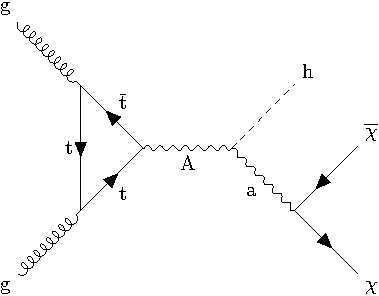
\includegraphics[width=0.525\textwidth]{Chapters/Theory/2HDMa.pdf}
\caption{The pseudoscalar A decaying into a Higgs boson, h, and a pseudoscalar a, which then decays to DM, $\chi$, in the 2HDM+a model.}
\label{fig:2hdma}
\end{figure}

\begin{equation}
    \ptmiss \simeq \frac{\sqrt{(m_\mathrm{A}^2-m_\mathrm{a}^2-m_\mathrm{h}^2)^2-4m_\mathrm{a}^2m_\mathrm{h}^2}}{2m_\mathrm{A}}
    \label{eq:ptmiss}
\end{equation}

Thus, in order to find this peak beyond the typical \ptmiss cut imposed in mono-Higgs searches, it must be that
\begin{equation}
    m_\mathrm{A} \gtrsim m_\mathrm{a} + \sqrt{m_\mathrm{h}^2+({\ptmiss}_{\text{cut}})^2}
\end{equation}

These measurements are expected to be mostly limited by statistical uncertainties through Run 2 of the LHC. As a result, they provide a particularly intriguing avenue to search for DM and are a search that would be interesting to project past the current Phase-1 analyses.

\section{Z\texorpdfstring{$'$}{'} Models}
\label{section:Z'}
Another promising class of simplified dark matter models are ones that propose an additional neutral vector mediator, typically referred to as \Zp. One particular \Zp model that has been investigated recently is the "baryonic Z" model~\cite{barZ2014}. In this model, the baryon number $B$ is gauged and \Zp is a gauge boson of a $U(1)_B$ symmetry. Adding this symmetry would predict additional stable baryons that would make ideal DM candidates. This theory would add interactions between fermionic DM and the SM by adding the following terms to the SM Lagrangian density
\begin{equation}
    g_q\bar{q}\gamma^\mu q\Zp_\mu + g_\chi\bar{\chi}\gamma^\mu\chi\Zp_\mu
\end{equation}

where $g_q = g_B/3$ and $g_\chi = B_\chi g_B$ with $g_B$ as the $U(1)_B$ gauge coupling and $B_\chi$ as the baryon number of the DM candidate. Notably, \Zp does not couple with leptons.

Similar to the Standard Model, the $U(1)_B$ symmetry is broken by a Higgs mechanism, which gives mass to the \Zp boson and leaves a physical particle, the baryonic Higgs h$_B$. There is an interaction between the baryonic Higgs and the baryonic Z, which adds the following term to the SM Lagrangian density
\begin{equation}
    \frac{1}{2}m_\Zp^2(1+\frac{h_B}{v_B})^2\Zp_\mu\Zp^\mu
\end{equation}
where $v_B$ is the VEV of the baryonic Higgs field and $m_\Zp$ is the \Zp mass. h$_B$ also mixes with the SM Higgs, given by the following Lagrangian density term
\begin{equation}
    \frac{m_\Zp^2\sin\zeta}{v_B}
\end{equation}
where $\zeta$ is the h-h$_B$ mixing angle. 

In total, this model has six parameters: $g_q$, $g_\chi$, $m_\Zp$, $m_\chi$, $v_B$, and $\zeta$. Similar to the 2HDM+a model, a variety of searches can provide constraints on the parameter space. In particular, searches that probe a variety of mono-Higgs and \ptmiss final states can provide constraints on the model parameters.

There are also \Zp models that incorporate elements of 2HDMs. One proposal suggests an extension of the SM by a $U(1)_\Zp$ symmetry with a \Zp gauge boson~\cite{Z2hdm2014}. Additionally, there are two Higgs doublets in this model, which behave in an analogous manner to the doublets in the 2HDM+a model, leading to the rise of five bosons: H, h, A$^0$, and H$^\pm$. The A$^0$ boson couples with fermionic DM, while the Higgs mechanism leads to mixing between the Z and \Zp mass states. 

The parameters of this model are the mixing angles $\beta$ and $\alpha$; the masses of the introduced particles $m_\Zp$, $m_\mathrm{h}$, $m_\mathrm{H}$, $m_{\mathrm{A}^0}$, $m_{\mathrm{H}^\pm}$, and $m_\chi$; and the couplings $g_\Zp$ and $g_\chi$. However, in the alignment limit, described previously, $m_\mathrm{h}$ is taken to be that of the SM Higgs and $\alpha = \beta-\frac{\pi}{2}$. Once again, mono-Higgs final states can lead to constraints on these parameters, although this model also has additional constraints from electroweak precision measurements and di-jet final states.
\chapter{The CMS Detector}
The Large Hadron Collider (LHC) is a particle accelerator and collider located in a 26.7 km tunnel underneath Geneva, Switzerland~\cite{Evans_2008}. The LHC is designed to operate at center-of-mass energies up to $\TeV{14}$, although these energies have only been reached recently. Protons can reach these energies more easily than electrons, which the predecessor to the LHC collided, because they lose relatively less energy when they are accelerated. The LHC consists of two rings with beams moving in opposite directions. These rings cross over at four different interaction points, where the main detectors at the LHC are positioned. Owing to the $\SI{3.7}{\m}$ diameter of the tunnel, there is not enough space for two separate magnet rings and instead a two-bore magnet is used. This magnet, comprised of niobium-titanium superconductors, is cooled to $\SI{2}{\kelvin}$ by superfluid helium to maintain a magnetic field of $\SI{8}{\tesla}$. This allows for the high-energy proton-proton collisions necessary for the work of the main detectors. 

At the LHC, the number of events per second is given by 
\begin{equation}
    N_\text{event} = L\sigma_\text{event}
\end{equation}
where $\sigma_\text{event}$ is the cross-section of the event and $L$ is the luminosity. The luminosity itself can be expressed in terms of parameters of the beam as
\begin{equation}
    L = \frac{N_b^2n_bf_\text{rev}\gamma_r}{4\pi\epsilon_n\beta^*}F
\end{equation}
where $N_b$ is the number of particles per bunch (a grouping of protons in the beam), $n_b$ is the number of bunches per beam, $f_\text{rev}$ is the frequency of revolution, $\gamma_r$ is the Lorentz factor, $\epsilon_n$ is the normalized transverse beam emittance, $\beta^*$ is the Beta function at the collision point, and $F$ is percentage by which the luminosity is reduced due to the beam crossing angle $\theta_c$. The current operating luminosity of the LHC is around $\SI{2d34}{\cm^{-2}\s^{-1}}$.

In order to increase the amount of data collected by the detectors in the LHC, the collider is being upgraded to increase the luminosity~\cite{Contardo:2020886}. The magnets that focus the beams in the LHC will be replaced and the bunch overlap in the optimization region will be optimized. This will allow the luminosity to increase to a maximum of $\SI{2d35}{\cm^{-2}\s^{-1}}$, although the typical operating luminosity will be $\SI{5d34}{\cm^{-2}\s^{-1}}$. This will increase the PU from 25 to 140 under mean conditions, with a peak of 200.

\section{The CMS Detector}
One of the main detectors at the LHC is the Compact Muon Solenoid (CMS). The technical specifications of CMS are summarized below. For a more in-depth description of the detector, see~\cite{Collaboration_2008}. \cref{fig:cms} presents a schematic view of the detector.

\begin{figure}[ht]
    \centering
    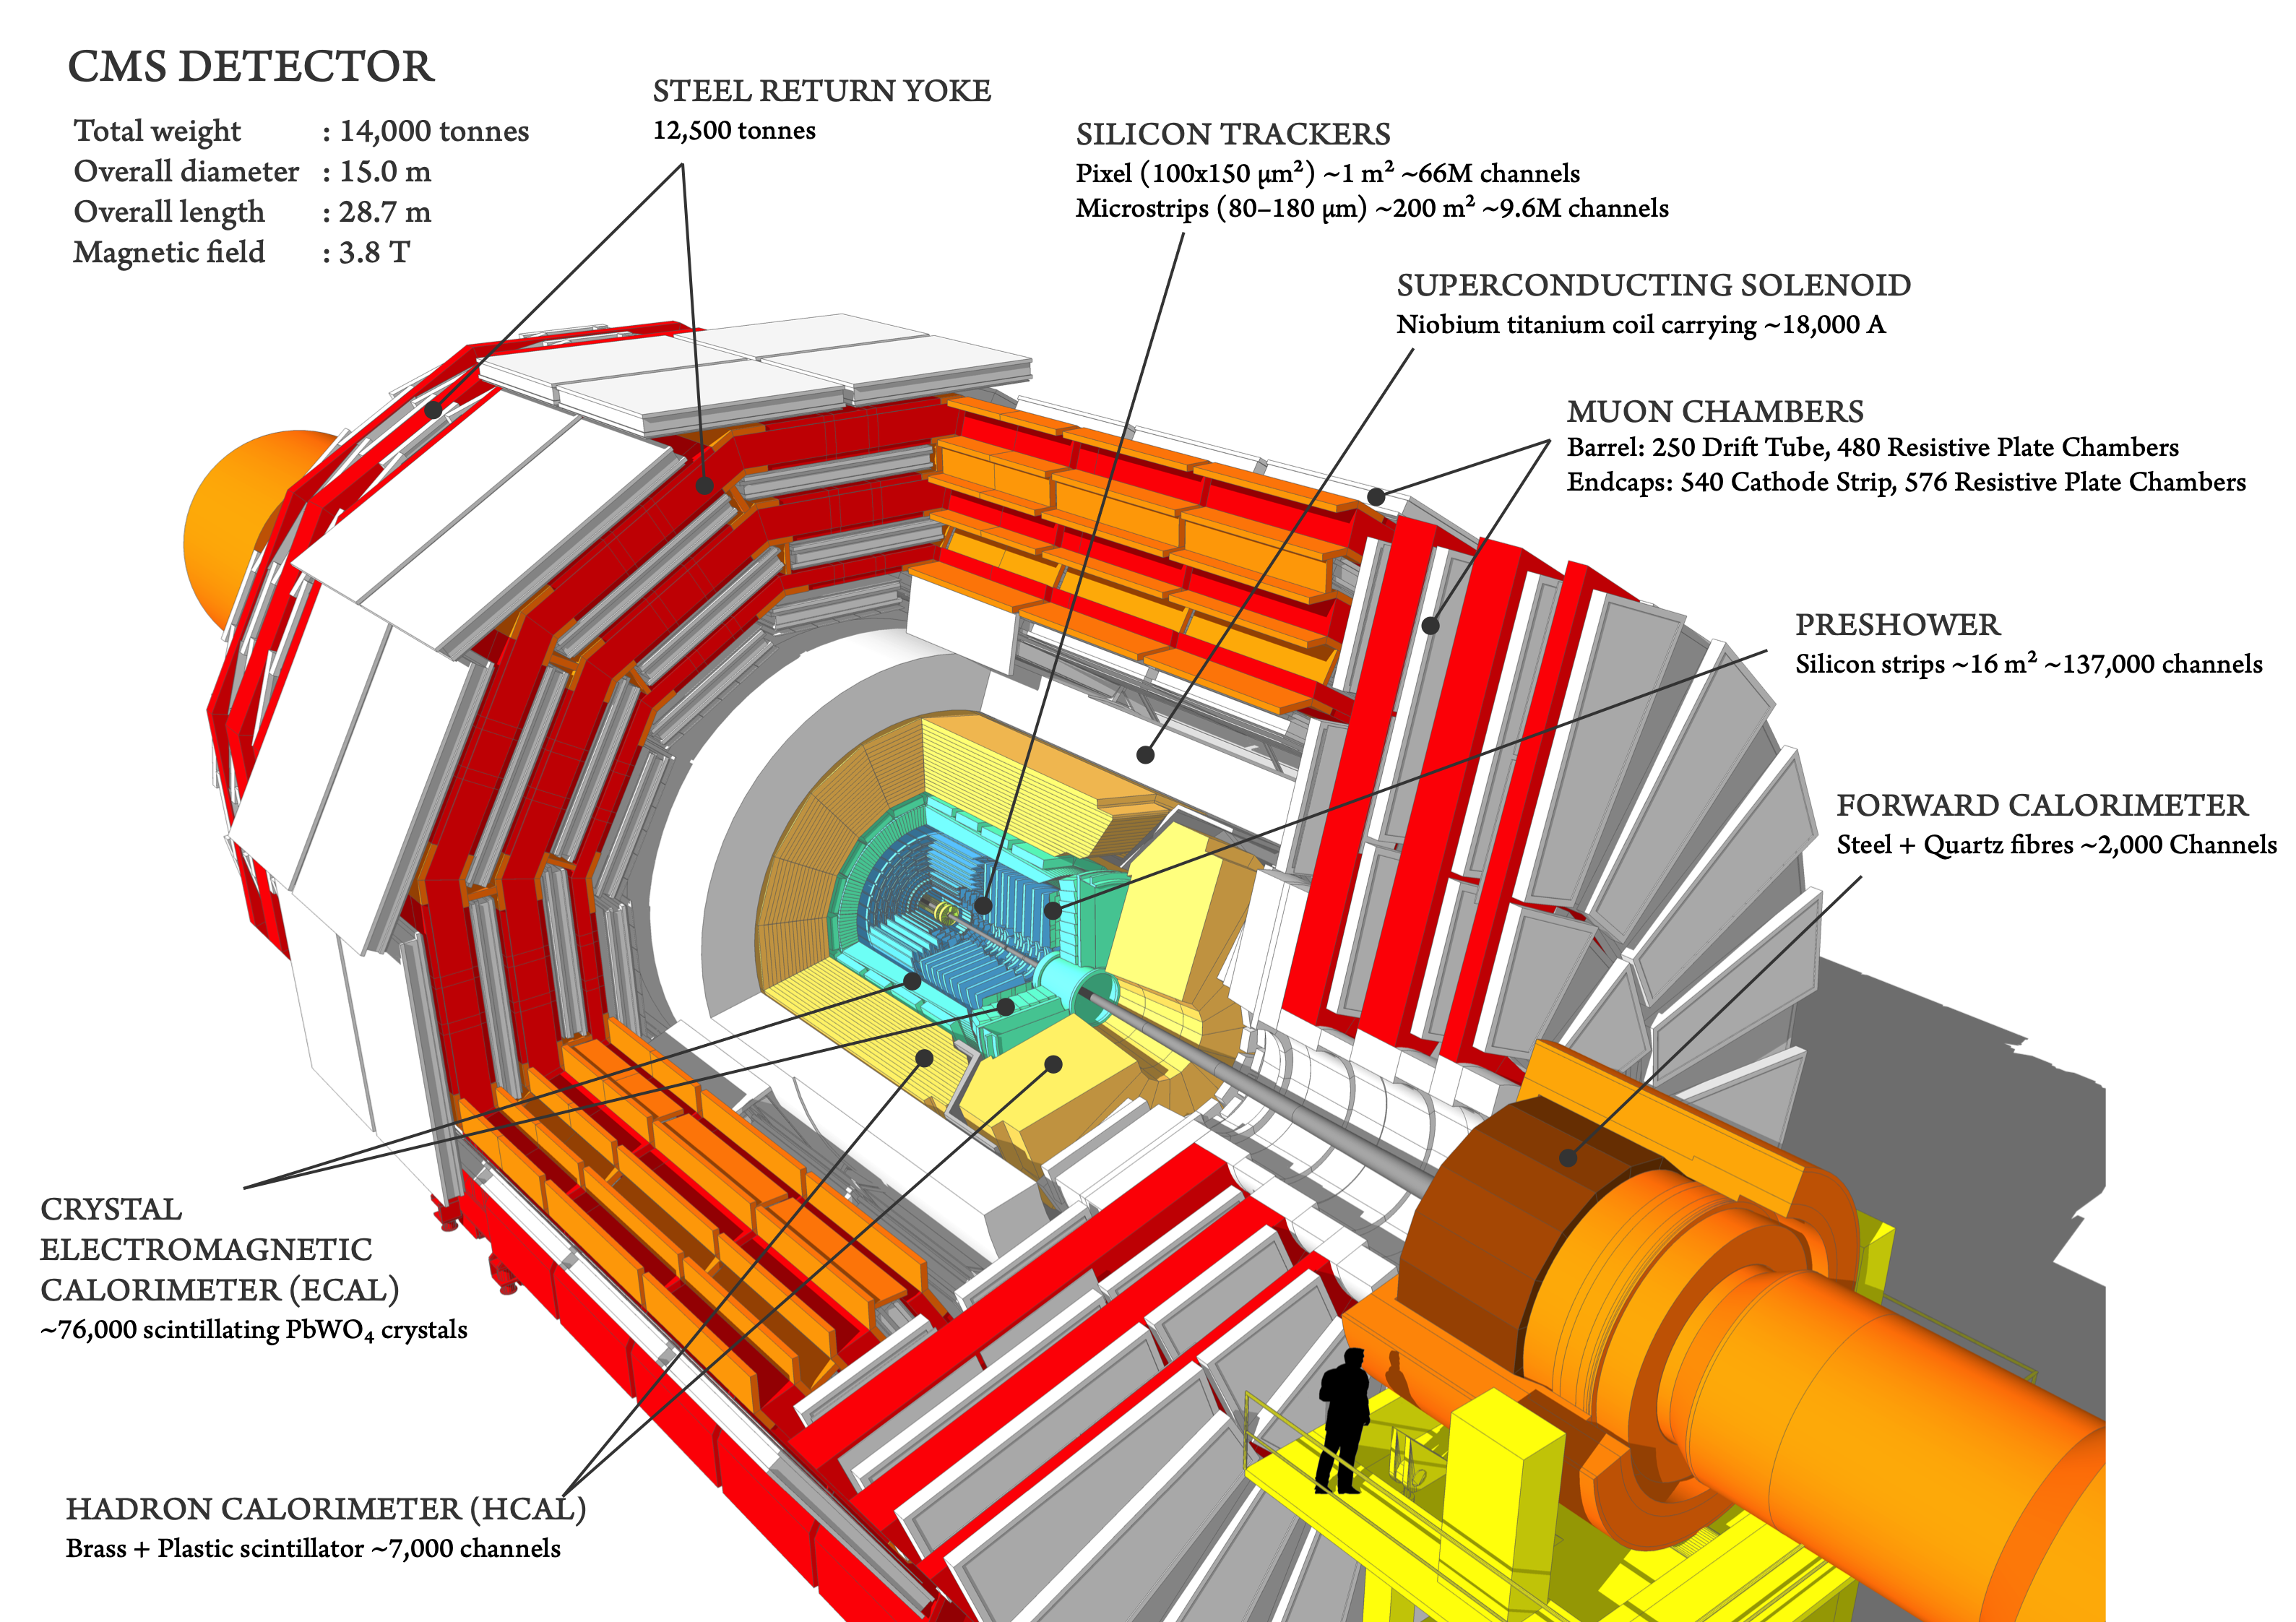
\includegraphics[width=0.75\textwidth]{Chapters/CMS/cms_160312_02.png}
    \caption{The CMS detector at the LHC in CERN~\cite{Sakuma_2014,Sakuma:2665537}.}
    \label{fig:cms}
\end{figure}

The main part of the CMS detector is $\SI{21.6}{\m}$ long and $\SI{14.6}{\m}$ in diameter, with a total weight of around $12500$ metric tons. The central feature of the detector is the titular solenoid, which can provide magnetic fields of strength up to $\SI{4}{\tesla}$. The superconducting magnet is $\SI{12.5}{\m}$ long with a diameter of $\SI{6}{\m}$. The main function of the solenoid is to cause charged particles in the detector to curve, allowing for measurement of their charge and momentum. Inside of the solenoid are the silicon tracker, the electromagnetic calorimeter (ECAL) and the hadron calorimeter (HCAL). Outside of the solenoid are a system of detectors designed for identifying and determining the properties of muons. Information from all these systems is taken by the CMS trigger for further processing before being stored. 
In the detector, the $y$-axis points vertically upward, the $x$-axis points radially inward towards the center of the LHC, and the $z$-axis points in the beam direction. The typical coordinates used for tracking objects in the detector are the angle $\phi$ from the $x$-axis in the $x$-$y$ plane, the distance $r$ in the $x$-$y$ plane, and the pseudorapidity $\eta$ measured as $\ln\tan(\theta/2)$, where $\theta$ is the polar angle measured from the $z$-axis.
It is common to refer to distances in the detector using the variable $R$, which is equal to $\sqrt{\eta^2+\phi^2}$.
The transverse components of the energy and momentum are calculated from the $x$ and $y$ components.

The innermost component of the detector is the tracker, which is $\SI{5.8}{\m}$ long and $\SI{2.5}{\m}$ in diameter. In the barrel of the solenoid, the tracker has three layers of silicon pixel detectors, followed by ten layers of silicon micro-strip detectors. Four of those layers comprise the tracker inner barrel (TIB) with thinner strips, while the remaining six are the tracker outer barrel (TOB) with thicker strips. The endcaps of the pixel detector have two disks of pixel detectors, while each endcap of the TIB have three disks of silicon strips. Lastly, there are nine endcap disks of silicon strips that bookend the entire tracker. Signals from the silicon detectors are read out by a sequence of chips.
The silicon tracker is able to measure vertex information and the \pt of physics objects with high precision and granularity. For high-momentum tracks, the latter can be measured with a resolution of 1-2\% up to $|\eta| = 1.6$. Although information from the tracker is not fed into the level-one (L1) trigger, it is part of the high-level trigger (HLT).

Moving radially outward, the next section of the detector is the electromagnetic calorimeter (ECAL). The ECAL is comprised of lead tungstate crystals. There are approximately 61000 of these crystals in the barrel of the ECAL, which covers a pseudorapidity of $|\eta| < 1.479$. There are around $7000$ crystals in each endcap, which cover the pseudorapidities between $|\eta| = 1.479$ and $|\eta| = 3.0$. When an electromagnetic particle passes though the ECAL, the crystals scintillate. The photons from these scintillations are detected by silicon avalanche photodiodes (APDs) in the barrel and by vacuum phototriodes (VPTs) in the endcaps. The ECAL electronics then report the energy deposited in a five-by-five section of the ECAL called a tower. Because the intensity of the scintillation is dependent on the temperature of the crystals, the ECAL is kept at $\SI{18}{\degreeCelsius}$.

Between the ECAL and the solenoid is the hadron calorimeter (HCAL). The HCAL is comprised of layers of brass absorbers and scintillating materials. Particles that hit the brass absorbers create a shower of secondary particles that cause the scintillators to emit photons. These photons are then detected by hybrid photodiodes (HPDs). The barrel of the HCAL (HB) covers up to $|\eta| = 1.3$. It is split into two halves with a total of 36 wedges, each of which are divided further into 4 $\phi$ sections. The endcap of the HCAL (HE) covers $1.3 < |\eta| < 3.0$. Because of the limited space between the ECAL and solenoid, in addition to the HB and HE, there is also a calorimeter outside the solenoid called the outer calorimeter (HO). The final piece of the HCAL is the forward calorimeter (HF) which extends the pseudorapidity range up to $|\eta| = 5.2$. The HF uses quartz fibers as its scintillators, whose photons are then read by photomultiplier tubes (PMTs).

The final major detector system is the set of detectors focused on identifying muons, determining kinematic information such as their \pt, and feeding information to the trigger. The muon system is a key part of CMS, as many important processes have muon final states. The barrel region of the muon system is comprised of drift tube (DT) chambers. There is not as much muon or background activity in the barrel, but closer to the beam the rate of activity increases, necessitating the use of the more precise cathode strip chambers (CSCs). In addition to being more segmented, the CSCs also fire faster than the DTs and are more resistant to radiation. The CSCs are used for pseudorapidities $0.9 < |\eta| < 2.4$. The CSCs are comprised of 6 anode wire plates which are sandwiched between 7 cathode wire plates. Particles that hit the anodes cause a shower of electrons which are drawn to the cathodes. The final muon subsystem is the resistive plate chambers (RPCs) which are present in both the barrel and endcaps, encompassing $|\eta| < 1.9$. The RPCs add additional information by being fast to respond, giving clear timing information. However, they are spatially coarser than the other detectors.

The information gleaned by the detector systems is fed into the triggers. Owing to the vast quantity of events taking place in the detector, most of these events cannot be stored. The trigger determines which of these events should be read out. The first trigger level is the level-one (L1) trigger, which is comprised of hardware in the detector systems. After events are processed by the L1 trigger, the high-level trigger (HLT) uses software to further determine which events should be stored offline. 
The L1 trigger begins with local triggers from energy deposits in the calorimeters and track hits in the muon chambers. This information is then fed into the regional triggers, which form particle object candidates and rank them. The regional muon trigger (RMT) determines tracks from the segments in the muon system, while the regional calorimeter trigger (RCT) determines electron and photon candidates, calculates some information for the muon candidates, and determines the tau veto. The global muon trigger takes information from the regional muon triggers to create muon candidates. The global calorimeter trigger creates jet candidates using a clustering technique. It also calculates global properties such as $E_\mathrm{T}$, \ptmiss, and $H_\mathrm{T}$. Information from this trigger level is fed into the global trigger, which determines which events to reject and which to forward to the HLT. 
The HLT takes on a wider array of information than the L1 trigger, allowing it to perform calculations similar to those done in offline analysis. This further reduces the number of stored events by not reading events with few valid or interesting candidates.

\section{CMS Phase-2}
\label{section:phase2}
In order to facilitate the taking of data during the HL-LHC era, CMS will undergo a series of upgrades referred to as CMS Phase-2. The overall goal of the upgrades is to ensure that the detector can handle the increase in pileup and radiation from the increased luminosity.

The L1 trigger will have its rate increased to $\SI{750}{kHz}$ and its latency increased to $\SI{12}{\us}$~\cite{CERN-LHCC-2020-004}. The HLT will have an upgraded rate of $\SI{7.5}{kHz}$.

The tracker system of CMS will be replaced entirely due to the high amount of radiation that will occur during Phase-2~\cite{CERN-LHCC-2017-009}. In place of the old tracker there will be an Outer Tracker (OT) that will help provide tracking information to the L1 trigger by rejecting tracks below a certain \pt. This will be done using \pt modules comprised of either two strip sensors or a strip and a macro-pixel sensor. These modules must be radiation resistant, due to the increased luminosity at the HL-LHC. The Inner Tracker (IT) will be comprised of thin silicon pixels that are designed for the increased radiation tolerance and granularity required of the Phase-2 IT. The IT is designed to be replaceable during shutdowns, due to the high amount of radiation damage that it will incur. Owing to the trigger upgrades described earlier, the tracker electronics will also be upgraded to work with those upgrades and allow for input from the tracker to the L1 trigger. Finally, the geometry of the tracker will be enhanced, allowing tracking up to pseudorapidities around $|\eta| = 4$.

Further improvements to CMS will occur in the barrel. As in the tracker, the electronics of the electromagnetic calorimeter (ECAL) will be upgraded to function with the improved trigger~\cite{CERN-LHCC-2017-011}. In particular, the L1 trigger will receive information from the individual lead tungstate crystals, as opposed to from the towers, to enable better track matching. The electronic upgrades, along with cooling the ECAL from $\SI{18}{\degreeCelsius}$ to $\SI{9}{\degreeCelsius}$, will also reduce the noise in the ECAL. The hadronic calorimeter (HCAL) will also have its electronics upgraded for compatibility with the trigger. The endcap calorimeters will be replaced by the HGCAL, which will be designed to withstand the heavier radiation of the HL-LHC~\cite{CERN-LHCC-2017-023}. 

As with the other CMS systems, the muon system electronics must be upgraded to function with the improved trigger~\cite{CERN-LHCC-2017-012}. Additionally, the geometric acceptance of the muon system will be increased to around $|\eta|=2.8$ by use of resistive plate chambers (RPCs) and gas electron multipliers (GEMs).

The final main upgrade to CMS is the inclusion of a minimum ionizing particle timing detector (MTD)~\cite{CMS:2667167}. In order to mitigate the effects of the increased PU of the HL-LHC, it is useful to be able to differentiate vertices not just in space but also in time. The MTD is split into two regions: the Barrel Timing Layer (BTL) covering $|\eta| < 1.5$ between the OT and the ECAL and the Endcap Timing Layer (ETL) covering $1.6 < |\eta| < 3.0$ in front of the endcap calorimeter. The BTL will consist of scintillating cerium-doped lutetium-yttrium oxyorthoscillicate crystals read out by silicon photomultipliers. The ETL will use silicon devices that can better withstand the radiation in the endcaps. The MTD will have a timing resolution of $\SI{30}{\ps}$ that comes from the detection of two hits per track in the various detection devices.

\chapter{Previous Searches}
As mentioned above, there are many theoretical motivations to study final states at the LHC involving h+\ptmiss. These final states provide some of the best ways to further constrain the parameter space offered by a wide variety of simplified DM models. Studying this final state can help lead to conclusions about the viability of indirect DM detection of these models. One subset of h+\ptmiss searches are those involving decays of the observed Higgs to a b quark-antiquark pair. This is a useful decay to look at because it is the most common Higgs decay~\cite{Zyla:2020zbs}. Another common Higgs decay to observe is h $\to\gamma\gamma$, since the di-photon decay tends to stand out background processes, even if it occurs at a much less frequent rate.

There have been several experimental searches for this state at the LHC. In one recent analysis, the CMS Collaboration used $\fbinv{35.9}$ of data collected in 2016 to search for dark matter in association with h $\to$ b$\bar{\mathrm{b}}$ decays~\cite{cms:hbb2019}. This search was motivated by the possibility of a coupling between the Higgs and theorized particles that would also couple to the DM sector, allowing further probing of DM-SM coupling. The search was analyzed through two frameworks. In the first, the observed Higgs is assumed to be the CP-even scalar h of the 2HDM+a model discussed in \cref{section:2hdma}. In the second framework, the observed Higgs interacts with a Z$'$ gauge boson that can decay to a dark matter candidate, as described in \cref{section:Z'}.

The analysis used the particle-flow (PF) algorithm~\cite{cms:pf2017} for object reconstruction. In order to find suitable Higgs candidates, the Cambridge-Aachen algorithm~\cite{cms:2009lxa} with distance parameter 1.5 was used to reconstruct jets likely produced by multiple quarks (CA15 jets), such as the two b quarks decaying from the Higgs. The analysis also formed jet objects using the anti-$k_{T}$ algorithm~\cite{ak2008} with a distance parameter of 0.4. The pileup per particle identification (PUPPI) algorithm~\cite{puppi2014} was used to avoid issues arising from pileup. The mass of the jet is calculated after using the soft-drop (SD) jet grooming algorithm~\cite{sd2014}. The final main variable used with the CA15 jets was a modified tagging variable N$_2^\text{DDT}$. The analysis identified several lepton objects through kinematic variables and identification requirements for use in eliminating background events. Here, the \ptvecmiss is calculated as the negative vector sum of the \pt of all reconstructed PF objects.

In order to focus in on the aforementioned final state, the analysis looked at events with high \ptmiss, no leptons or photons, and a CA15 jet. The analysis also defined several control regions in order to estimate the \ptmiss distribution of the main background processes, which are Z bosons produced in association with initial state jets, W bosons produced in association with initial state jets, and t$\bar{\mathrm{t}}$.
In all regions, it was required that the CA15 jet have $\pt > 200$ GeV, $|\eta| <2.4$, $100<m_{\text{SD}}<\GeV{200}$, and N$_2^\text{DDT} < 0$. There was also a requirement that the \ptmiss be greater than \GeV{200}. Finally, there were requirements that the azimuthal angle $\varphi$ between the AK4 jets and the \ptmiss be greater than 0.4 and that there were fewer than 2 AK4 jets with $R$ between them and the CA15 jet greater than 1.5.

The signal and background contributions were extracted with a simultaneous binned likelihood fit.
A variety of systematic uncertainties were assigned as nuisances, including b quark tagging/mistagging efficiencies, transfer factor statistical uncertainties, and the CA15 jet energy. No significant excess over the SM expectation was observed.

Using the 2HDM+a model, the analysis scanned and found excluded regions for $m_\mathrm{A}$, $\sin\theta$, and $\tan\beta$. With $\sin\theta=0.35$, $\tan\beta = 1$, $m_\mathrm{a}=\GeV{150}$, $m_\chi = \GeV{10}$, and $m_\mathrm{A}=m_\mathrm{H}=m_{\mathrm{H}^{\pm}}$, $m_\mathrm{A}$ between $500$ and $\GeV{900}$ are excluded. With $\tan\beta = 1$, $m_\mathrm{a}=\GeV{200}$, $m_\chi = \GeV{10}$, and $m_\mathrm{A}=m_\mathrm{H}=m_{\mathrm{H}^{\pm}} = \GeV{600}$, $\sin\theta$ between 0.35 and 0.75 are excluded. Finally, with $\sin\theta=0.35$, $m_\mathrm{a}=100$ ($150$) $\GeV{}$, $m_\chi = \GeV{10}$, and $m_\mathrm{A}=m_\mathrm{H}=m_{\mathrm{H}^{\pm}} = \GeV{600}$, $\tan\beta$ between 0.5 and 2.0 (1.6) are excluded. A summary of these results can be seen in \cref{fig:hbbmet20191}.

\begin{figure}[ht]
\centering
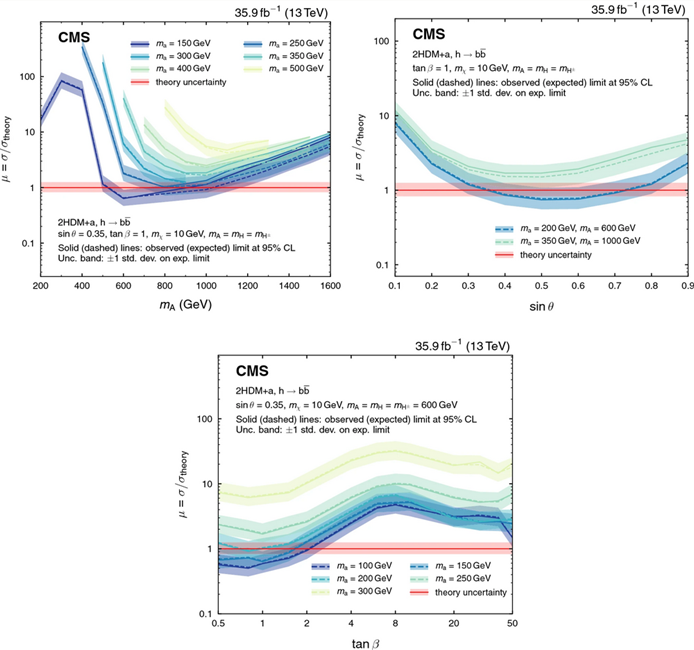
\includegraphics[width=0.8\textwidth]{Chapters/Experiment/2019hbbmet_results.png}
\caption{Upper limits on the 2HDM+a model of DM production in association with h $\to$ b$\bar{\mathrm{b}}$+\ptmiss obtained in~\cite{cms:hbb2019}. The theory uncertainty has been taken to be 20\%.}
\label{fig:hbbmet20191}
\end{figure}

Using the \Zp model, the analysis scanned and found excluded regions for $m_\Zp$ and $m_\chi$. For $m_\chi = \GeV{1}$, $m_\Zp$ is excluded up to $\GeV{1600}$. On the other hand, for $m_\Zp = \GeV{960}$, $m_\chi$ is excluded up to $\GeV{430}$. A summary of these results can be seen in \cref{fig:hbbmet20192}.

\begin{figure}[ht]
\centering
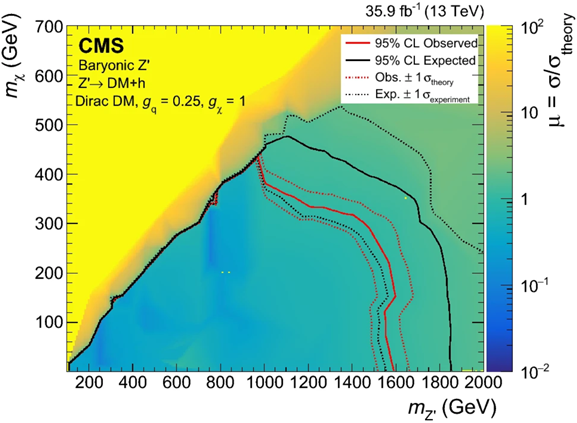
\includegraphics[width=0.6\textwidth]{Chapters/Experiment/2019hbbmet_results2.png}
\caption{Upper limits on the baryonic Z$'$ model of DM production in association with h $\to$ b$\bar{\mathrm{b}}$+\ptmiss obtained in~\cite{cms:hbb2019}.}
\label{fig:hbbmet20192}
\end{figure}

The ATLAS collaboration has published a couple of analyses examining the h $\to$ b$\bar{\mathrm{b}}$+\ptmiss final states in recent years, first using data gathered early in Run 2 of the LHC and then with the full dataset~\cite{atlas:hbb2017,atlas:hbb2021}. The latter search was interpreted through the 2HDM+a model as well as a model with an additional Higgs doublet and a \Zp boson.

For the 2HDM+a scenario, the $m_\mathrm{A}$-$m_\mathrm{a}$ parameter space was scanned for two values of $\tan\beta$. As mentioned in \cref{section:2hdma}, for smaller values of $\tan\beta$, the A pseudoscalar is most likely to couple to ah and t$\bar{\mathrm{t}}$. However, for larger values of $\tan\beta$, A is more likely to couple to b$\bar{\mathrm{b}}$. Thus, by scanning the parameter space with $\tan\beta=1$, events are more likely to be produced by gluon-gluon fusion, while scanning the space with $\tan\beta=10$ leads to more events produced by b$\bar{\mathrm{b}}$. For the gg ($\tan\beta=1$) initial state, with $g_\chi = 1$, $\sin\theta=0.35$, $m_\chi=\GeV{10}$, and $m_\mathrm{A}=m_\mathrm{H}=m_{\mathrm{H}^\pm}$ for $m_\mathrm{A}=\GeV{900}$, masses of a were excluded up to $\GeV{240}$, representing an improvement on previous results. For the b$\bar{\mathrm{b}}$ ($\tan\beta=10$) initial state, with $g_\chi = 1$, $\sin\theta=0.35$, $m_\chi=\GeV{10}$, and $m_\mathrm{A}=m_\mathrm{H}=m_{\mathrm{H}^\pm}$ for $m_\mathrm{A}=\GeV{1250}$, masses of a were excluded up to $\GeV{250}$, which are the first bounds established for these parameters. These results are pictured in \cref{fig:hbbmet20211}.

\begin{figure}[ht]
\centering
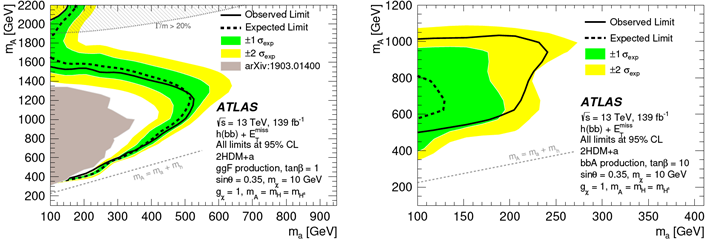
\includegraphics[width=\textwidth]{Chapters/Experiment/2021hbbmet_results.png}
\caption{Upper limits on the 2HDM+a model of DM production in association with h $\to$ b$\bar{\mathrm{b}}$+\ptmiss obtained in~\cite{atlas:hbb2021}. The solid (dashed) black lines give the observed 95\% CL (expected) limit, with the green and yellow bands giving the $1\sigma$ and $2\sigma$ uncertainties on the expected limit.}
\label{fig:hbbmet20211}
\end{figure}

For the \Zp-2HDM scenario, the $m_{\mathrm{A}^0}$-$m_\chi$ parameter space was scanned, with $g_z$ set to 0.8, $g_\chi=1$, $\tan\beta=1$, $m_\chi = \GeV{100}$, and $m_{\mathrm{A}^0}=m_\mathrm{H}=m_{\mathrm{H}^\pm}$. For $m_{\mathrm{A}^0} = \GeV{300}$, $m_\Zp$ values are excluded up to $\GeV{3000}$. These results are pictured in \cref{fig:hbbmet20212}.

\begin{figure}[ht]
\centering
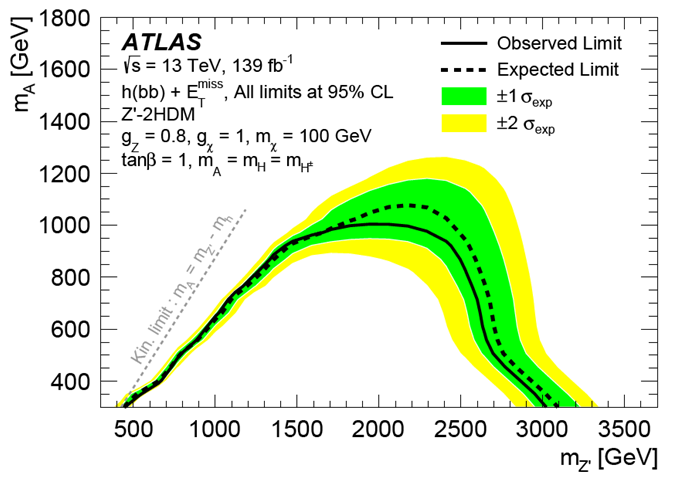
\includegraphics[width=0.6\textwidth]{Chapters/Experiment/2021hbbmet_results2.png}
\caption{Upper limits on the Z$'$-2HDM model of DM production in association with h $\to$ b$\bar{\mathrm{b}}$+\ptmiss obtained in~\cite{atlas:hbb2021}. The solid (dashed) black lines give the observed 95\% CL (expected) limit, with the green and yellow bands giving the $1\sigma$ and $2\sigma$ uncertainties on the expected limit.}
\label{fig:hbbmet20212}
\end{figure}
\chapter{Datasets}
\label{chap:datasets}
Most analyses at the LHC make use of simulations of events. Simulations are excellent tools for predicting backgrounds in analyses as well as modeling the observables of the targeted signal. Simulating events at the LHC or HL-LHC involves solving extremely complicated problems in QCD and thus requires a variety of software tools to be accomplished.

One method that makes this task easier is factorization, which lets the calculation be separated into different momentum regimes~\cite{Buckley_2011}. At high momentum are the hard processes, where partons of the incoming protons interact to form outgoing particles. The calculations for these processes can be done perturbatively. The next regime is the evolution from the hard processes to the low-momentum soft processes where hadrons form. This is typically simulated using a parton shower algorithm. The partons of this process form hadrons, but hadronization cannot be calculated perturbatively and is instead simulated using models. In each regime, Monte Carlo methods are used for calculation.

For a hard process, the cross section of a scattering process $ab\to n$ can be calculated by

\begin{equation}
    \sigma = \sum_{a,b}\int_0^1 \mathrm{d}x_a\mathrm{d}x_b\int f^{h_1}_a(x_a, \mu_F)f^{h_2}_b(x_b, \mu_F)\mathrm{d}\hat{\sigma}_{ab\to n}(\mu_F, \mu_R)
\end{equation}

where $f^h_a(x,\mu)$ are the parton distribution functions (PDFs) and $\hat{\sigma}_{ab\to n}(\mu_F, \mu_R)$ is the parton-level cross-sections of $a$, $b$ scattering into $n$. The PDFs depend on the momentum fraction $x$ of the parton $a$ of its parent hadron $h$ and on the factorization scale $\mu_F$. The parton-level cross-section depends on $\mu_F$ as well as the renormalization scale $\mu_R$ and the momenta of final state phase-space $\Phi_n$. The cross-section is calculated using the matrix element squared of the process. There is no one correct choice of $\mu_R$ and $\mu_F$, but one common choice is a scale $Q^2$ such that $\mu_F=\mu_R=Q^2$. Often $Q$ is chosen to be the mass of a particle or the \pt of a pair of massless particles.

To generate the 2HDM+a samples used in this thesis, \textsc{MadGraph5} v2.6.5~\cite{Alwall:2014hca} is used to simulate the hard scattering process by calculating the matrix elements at leading order (LO) in the perturbative QCD calculation. \textsc{MadGraph5} is also used to obtain the cross section of these processes. In creating these samples, some of the model parameters are fixed with $\sin\theta = 0.35$, $\tan\beta = 1$, and $m_\chi = \GeV{10}$. \textsc{MadGraph5} is also used to produce the W+jets, Z+jets, and multijet samples. In order to produce samples for Wh, Zh, and t$\bar{\mathrm{t}}$ events, the \textsc{Powheg}~\cite{Frixione_2007} tool is used to accurately simulate these events at next-to-leading order (NLO) in the perturbative QCD calculation.

\textsc{Pythia} v8 is then used in order to simulate both parton showering and hadronization~\cite{Sjostrand:2014zea}.
Finally, in order to simulate the Phase-2 detector, the \textsc{Delphes} v3.5.0 framework is used~\cite{deFavereau:2014dph,Selvaggi:2014mya,Selvaggi:2016ydq}.
\textsc{Delphes} allows for fast simulation of detector effects by reducing the complexity of aspects of the simulation. This is done by making some simplifying assumptions and by parametrizing the detector response.

A table of the name of the samples used in this thesis along with their cross-sections has been provided in \cref{app:samples}.
\chapter{Event Reconstruction and Selection}

\section{Physics Objects}
\label{section:objects}
The physics objects in this thesis are reconstructed using a modified particle flow (PF) algorithm for the \textsc{Delphes} parametrization of the detector geometry. The PF algorithm combines information from the tracker, the calorimeters, and the muon system to form PF candidates~\cite{cms:pf2017}.

The most crucial element of this thesis is identifying the Higgs boson decaying to two b quarks. Because quarks cannot exist independently, the b quarks will quickly hadronize. These hadrons show up in the detector through the tracks they make in the silicon tracker and the energy they deposit in the HCAL. The anti-$k_T$ clustering algorithm~\cite{ak2008} then combines the PF candidates from those tracks and HCAL hits to form jets. In particular, it forms AK4 and AK8 jets (so-called because they are clustered within radii of $R=0.4$ and $R=0.8$, respectively). As can be seen in \cref{fig:deltaRvspt}, b quarks from the decays of a high-momentum Higgs boson are more likely than not to be within $R=0.8$ from each other. As a result, AK8 jets that are reconstructed from the decays of such Higgs bosons will typically contain both b quarks in the jet radius. Accordingly, they are a key focus of this search since the signal will almost certainly be reconstructed as an AK8 jet. The extreme PU of the Phase-2 detector, described earlier, is accounted for with the Pileup Per Particle Identification (PUPPI) algorithm~\cite{puppi2014}.

Because of the limited extent of the tracker, AK4 and AK8 jets must be within $|\eta|$ of $3.0$. AK8 jets must have a \pt of at least $\GeV{200}$, while AK4 jets must have a \pt of at least $\GeV{30}$ . Both jets need to pass basic identification requirements~\cite{CMS-DP-2020-020} and are additionally removed if a lepton is contained within their radius, so as to prevent double-counting of jets that are also identified as leptons. The AK8 jet mass is calculated with the soft drop (SD) algorithm~\cite{sd2014}. It is important to note that, although AK4 jets and AK8 jets can be reconstructed from the same PF candidates, AK4 jets that are found within the AK8 jet cone are not removed. As a result, overlap between these objects is possible.

\begin{figure}[ht]
\centering
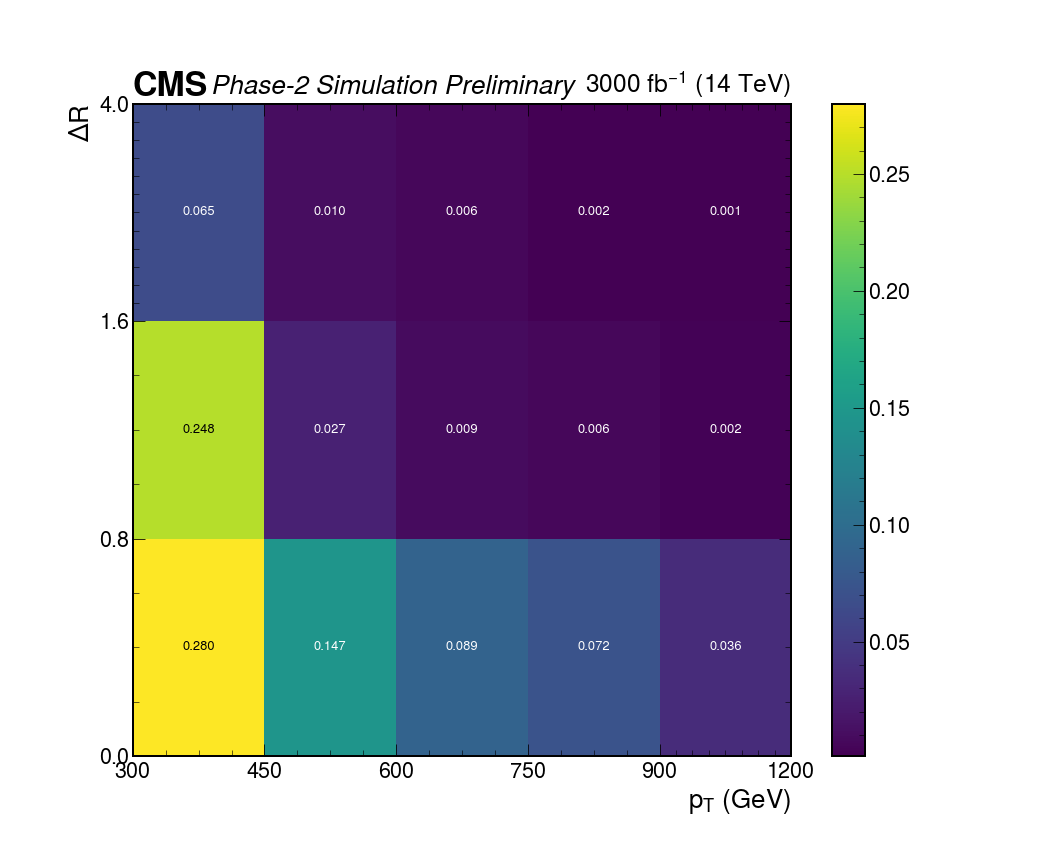
\includegraphics[width=0.845\textwidth]{Chapters/Strategy/b_DeltaR_vs_h_pt.png}
\caption{The $\Delta R$ between two generator-level b quarks against the \pt of the generator-level Higgs boson in events from a 2HDM+a signal with $m_\mathrm{A} = 1900$ GeV, $m_\mathrm{a} = 250$ GeV. The value in each bin in this histogram is the ratio of the counts in that bin to the overall yield.}
\label{fig:deltaRvspt}
\end{figure}

The \ptvecmiss is calculated using the vector sum of the \pt of the PF candidates, with inputs from the PUPPI algorithm to mitigate the effects of PU.

One tool often used in analyses that focus on particles such as the Higgs boson are heavy object taggers. These are algorithms created using machine learning techniques that excel at identifying objects such as the Higgs boson from a variety of similar looking backgrounds. In particular, taggers were developed during Run 2 of the LHC to identify AK8 jets that arise from Higgs decays to b$\bar{\mathrm{b}}$~\cite{CMS:2020mlt, Qu_2020}. Unfortunately, no such taggers are implementable for the \textsc{Delphes} framework. However, I anticipate that the accuracy of such taggers is likely to be at least as performant during the HL-LHC era.

Using fully simulated LHC Run 2 samples, the tagger efficiency is parametrized as a function of the AK8 jet \pt and $|\eta|$. The true efficiency of the tagger, when the tagger accurately identifies a Higgs boson, is calculated for events with generator-level Higgs bosons contained in the AK8 jet cone. The mistag efficiency, when the tagger mistakenly identifies a Higgs boson, is further parametrized by the number of b quarks in the AK8 jet cone. The efficiency is calculated by binning the simulated events in these variables, then calculating the efficiency in each bin according to \cref{eq:tageff}. A jet is considered tagged if it passes a working point based on the performance of the DeepAK8Jet mass-decorrelated h $\to$ b$\bar{\mathrm{b}}$ tagger against a multijet background. The efficiency is calculated on a sample-by-sample basis, owing to the sample-dependent nature of the tagger. A qualitative example of the mistag efficiencies for events with zero, one, or two b quarks in a semileptonic t$\bar{\mathrm{t}}$ sample is shown in \cref{fig:tagger}. After the tagger efficiency is calculated, it is then applied as a weight to the \textsc{Delphes} events as a function of the parametrized variables. The efficiency is calculated for each AK8 jet in the event as a function of \pt, $|\eta|$, and the number of b quarks and Higgs bosons in the AK8 jet cone. The weights for events with either no Higgs bosons or one or more Higgs bosons are then calculated according to the formulas given in \cref{eq:w0h,eq:w1h}.

\begin{equation}
    \epsilon = \frac{N_\text{tagged}}{N_\text{jets}}
    \label{eq:tageff}
\end{equation}

\begin{figure}[ht]
\centering
\begin{subfigure}[b]{0.33\textwidth}
         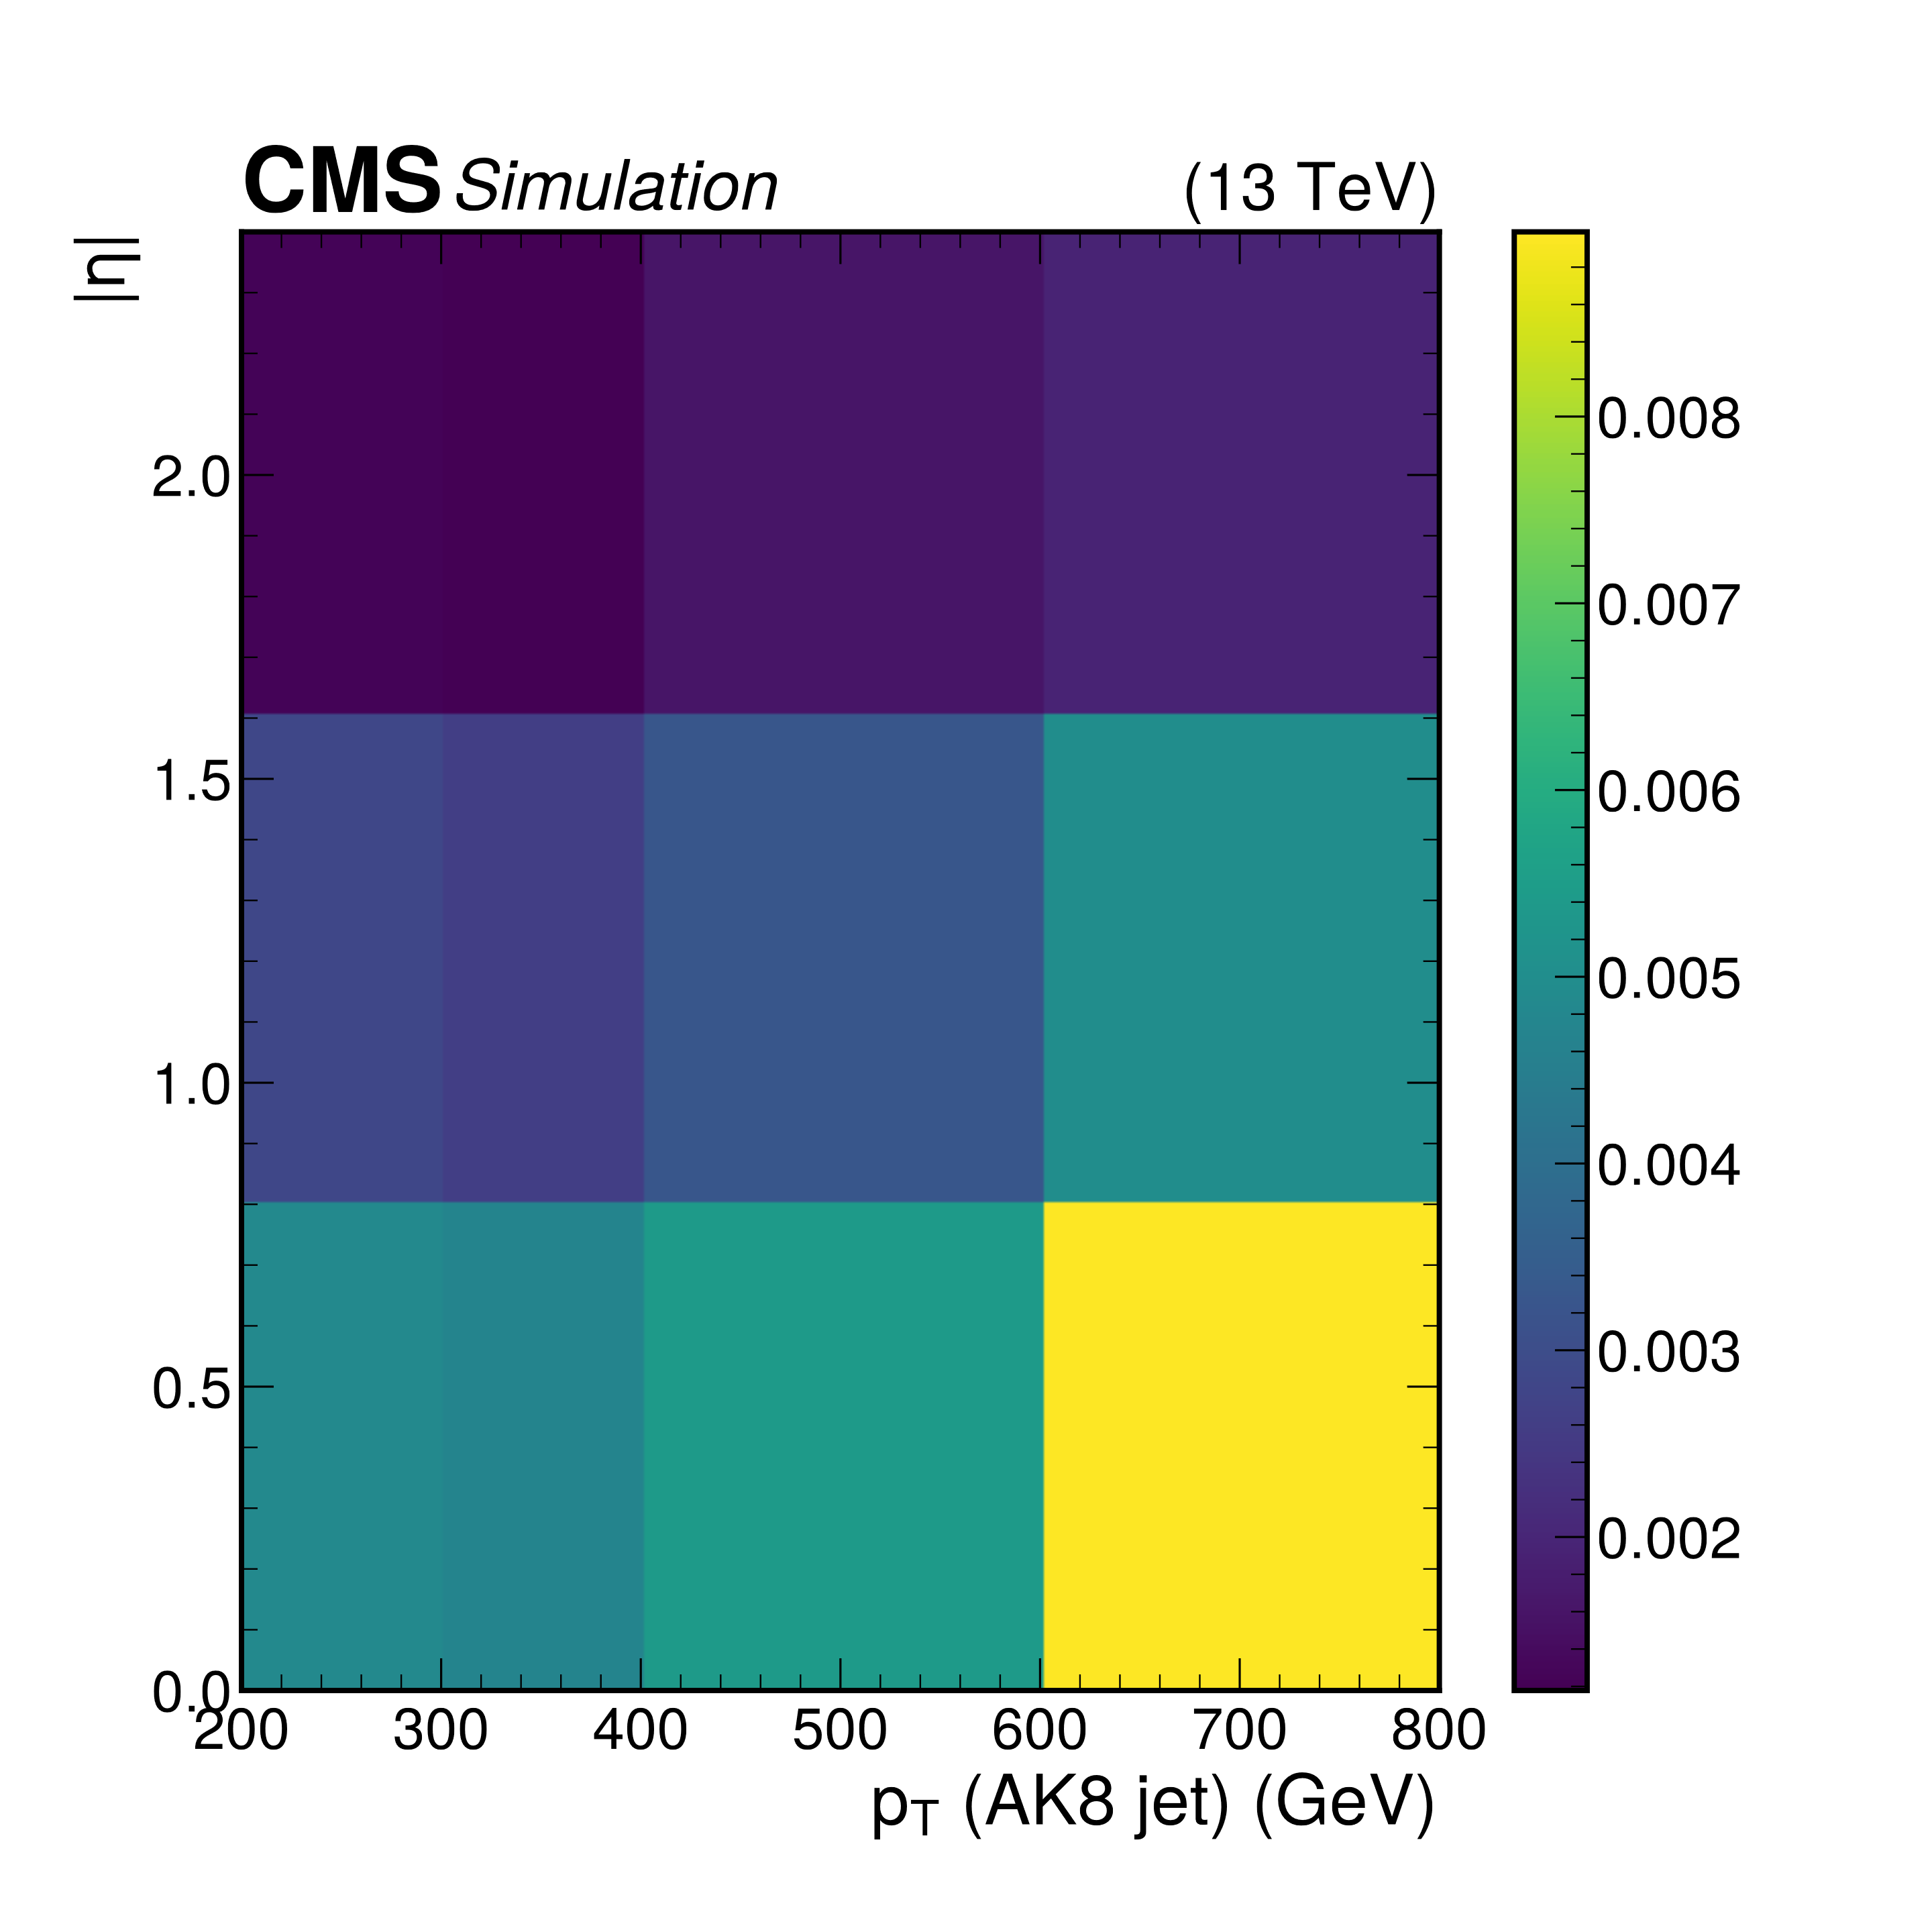
\includegraphics[width=\textwidth]{Chapters/Strategy/0b.png}
         \caption{The mistag efficiencies for zero b quarks.}
     \end{subfigure}
     \begin{subfigure}[b]{0.33\textwidth}
         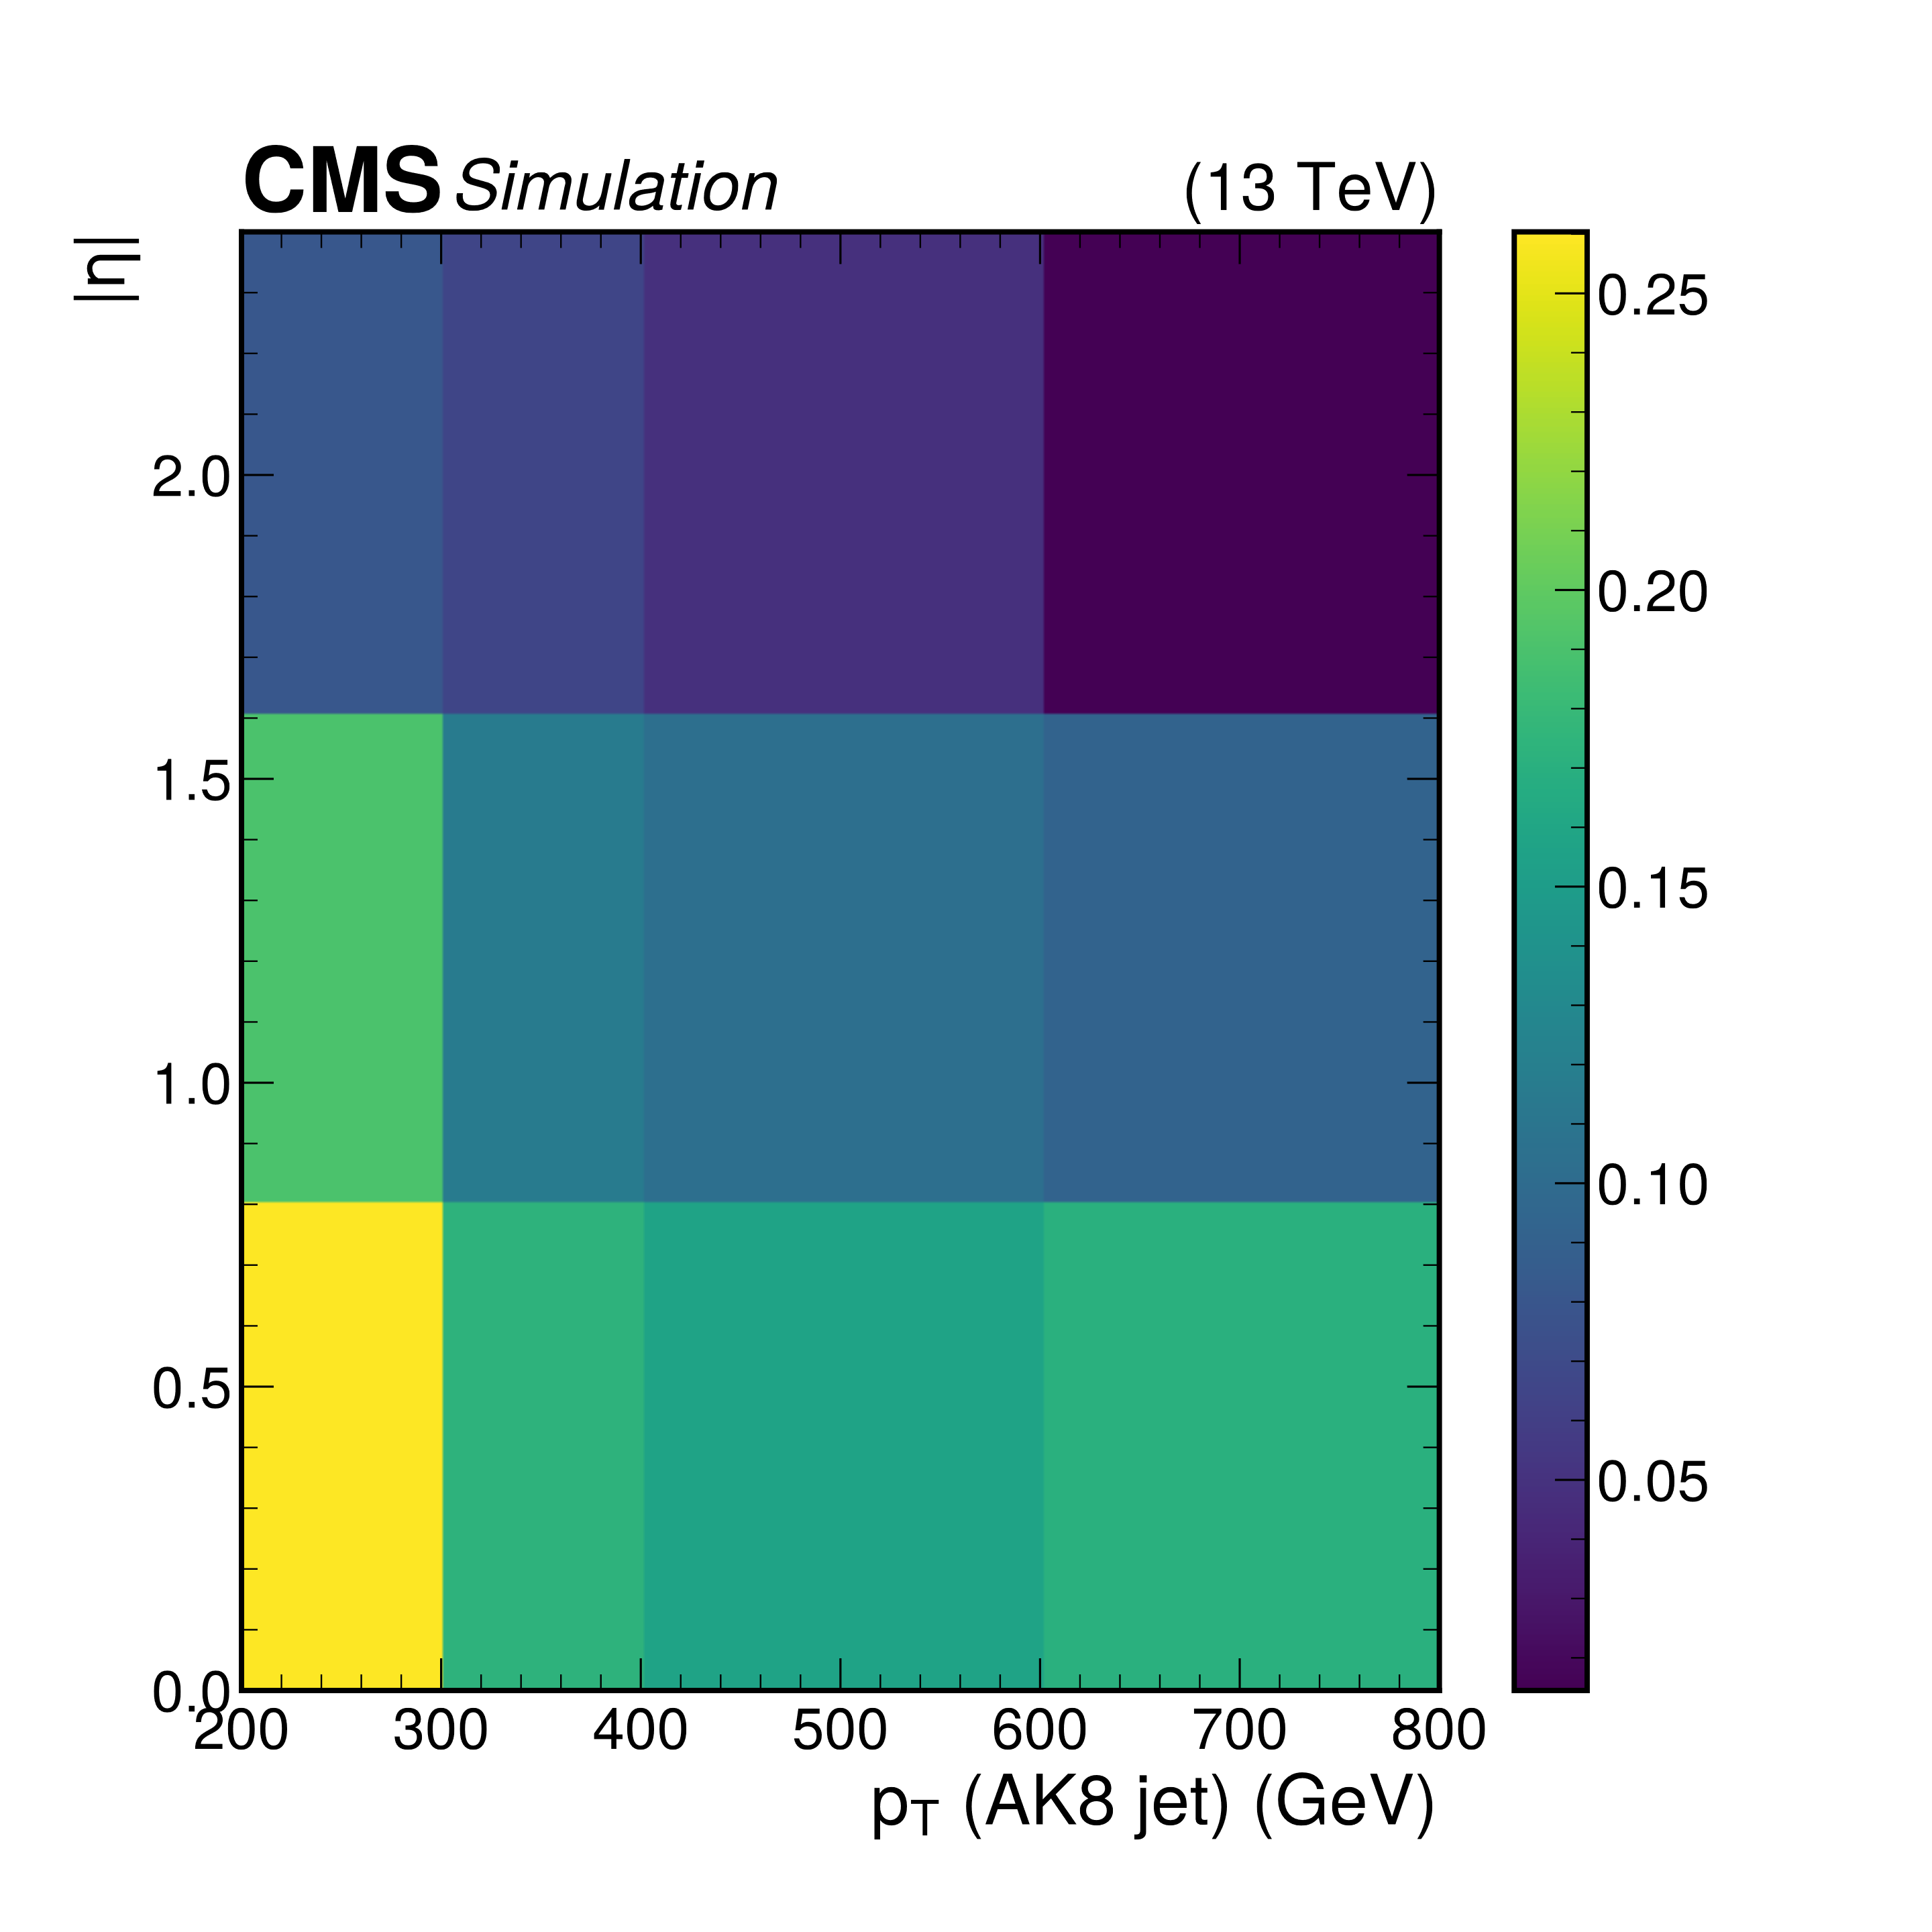
\includegraphics[width=\textwidth]{Chapters/Strategy/1b.png}
         \caption{The mistag efficiencies for one b quark.}
     \end{subfigure}
    \begin{subfigure}[b]{0.33\textwidth}
         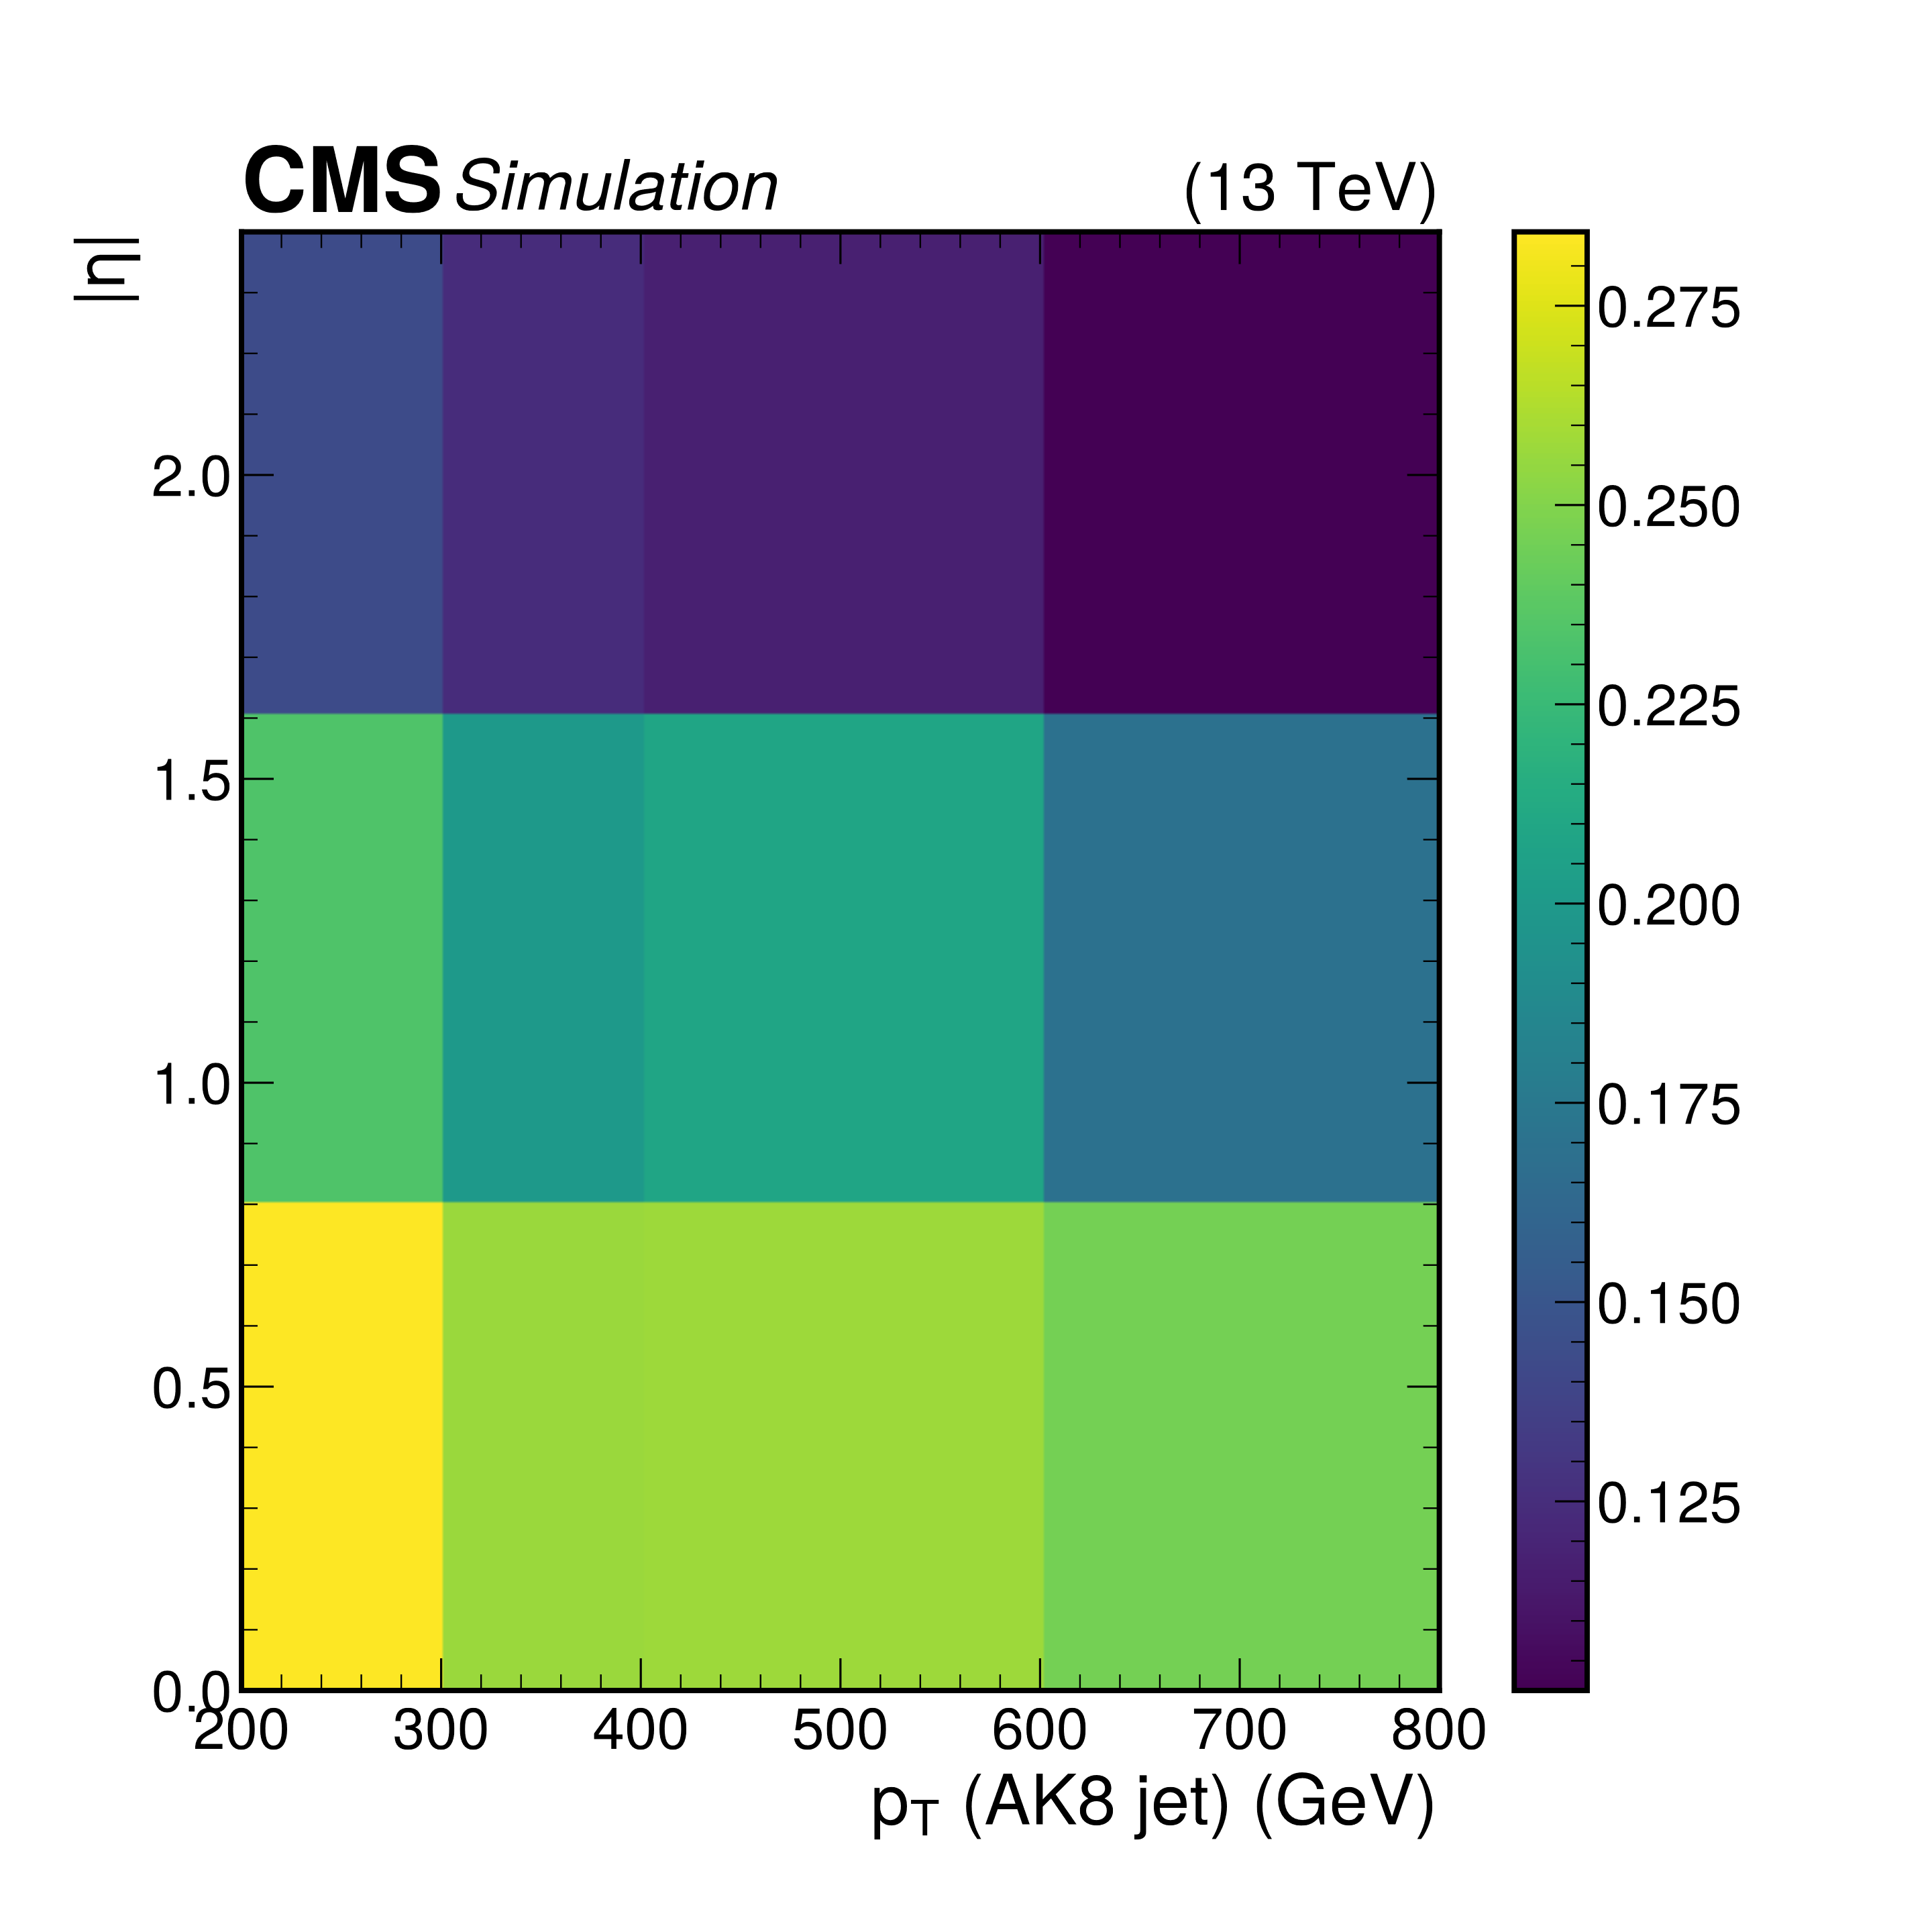
\includegraphics[width=\textwidth]{Chapters/Strategy/2b.png}
         \caption{The mistag efficiencies for two b quarks.}
     \end{subfigure}
\caption{\raggedright The mistag efficiencies of the Run 2 h $\to$ b$\bar{\mathrm{b}}$ mass-decorrelated DeepAK8Jet tagger in a semileptonic t$\bar{\mathrm{t}}$ sample. The efficiency has been parametrized as a function of \pt and $|\eta|$.}
\label{fig:tagger}
\end{figure}

\begin{equation}
    w(\text{0h}) = \prod_{i\in\text{\{AK8 jets\}}}(1-\epsilon_i)
    \label{eq:w0h}
\end{equation}

\begin{equation}
    w(\geq\text{1h}) = 1 - w(\text{0h})
    \label{eq:w1h}
\end{equation}

Leptons in the detector are reconstructed from their tracks and their deposits in the ECAL. Muons are additionally reconstructed using information from the muon system and taus can be reconstructed with deposits in the HCAL. Leptons represent an important part of the thesis because removing lepton final states eliminates a substantial portion of the background in this search. The Phase-2 detector is enormously beneficial in doing so, as it expands the geometric coverage of leptons in the detector. Electrons are required to have a \pt greater than $\GeV{10}$ and have $|\eta| < 3.0$. Muons are required to have a \pt greater than $\GeV{4}$ and have $|\eta| < 2.8$. Taus are required to have a \pt greater than $\GeV{30}$ and have $|\eta| < 3.0$. In addition, the leptons are required to pass identification and isolation restrictions. For electrons and muons, the relative isolation as defined in \cref{eq:irel} is required to be less than 0.3. The identification requirements for electrons and muons in \textsc{Delphes} are based on the identification requirements from the full simulation of the Phase-2 samples. The tau isolation requirements are based on machine learning tools designed to identify taus from jets. A summary of the object selections is given in \cref{tab:objdef}.

\begin{equation}
    \text{Iso}_{\text{rel}} = \frac{\sum \pt(\text{PUPPI particles within } R=0.3)}{\pt(\mathrm{e}, \upmu)}
    \label{eq:irel}
\end{equation}

\begin{table}[ht!]
  \centering
  \caption{Object selections as described in \cref{section:objects}}
  \begin{tabular}{|c|c|c|c|c|}
    \hline
    Object & \pt (GeV) $>$ & $|\eta|$ $<$ & Iso & ID WP \\
    \hline
    AK4 jet  & 30  & 3.0 &   & L \\
    AK8 jet  & 200 & 3.0 &   & L \\
    electron & 10  & 3.0 & L & L \\
    muon     & 4   & 2.8 & L & L \\
    tau      & 30  & 3.0 & L &   \\
        \hline
    \end{tabular}
    \label{tab:objdef}
\end{table}

 
\section{Event Selection}
Once objects in the detector have been reconstructed, the next step in the search is to remove as many events as possible that could contribute to the background of the signal region. The first few selections are aimed at targeting the final state of a Higgs boson decaying to b$\bar{\mathrm{b}}$ with high \ptmiss. First, the \ptmiss of each event is required to be greater than $\GeV{300}$. This requirement helps ensure that the events in the signal region are in the parameter space the search targets. Additionally, a Phase-2 analysis of this final state would need to use a high \ptmiss threshold in the HLT. As mentioned in the preceding section, one selection is to require that events have no leptons in them. Certain background events such as Z bosons produced in association with initial state jets or other modes of Higgs production can have final states with leptons, so this cut helps to remove much of the initial background. Events are required to have at least one AK8 jet, since signal events should have an AK8 jet from the Higgs decaying to b$\bar{\mathrm{b}}$. At least one AK8 jet in the event should have \pt greater than $\GeV{300}$. Events are also required to have at least 2 AK4 jets. This requirement helps to remove some of the multijet background. Finally, events are required to contain at least one Higgs-tagged AK8 jet. The AK8 jets are not tagged directly, but instead the weight for events with 1 or more Higgs bosons described in \cref{eq:w1h} is applied to all events. By comparing the $m_\text{AK8}$ distribution in a Run 2 sample between events that contained a tagged AK8 jet and events that were reweighted, it can be seen that the two are largely equivalent, as shown in \cref{fig:tagcheck}.

\begin{figure}[ht]
\centering
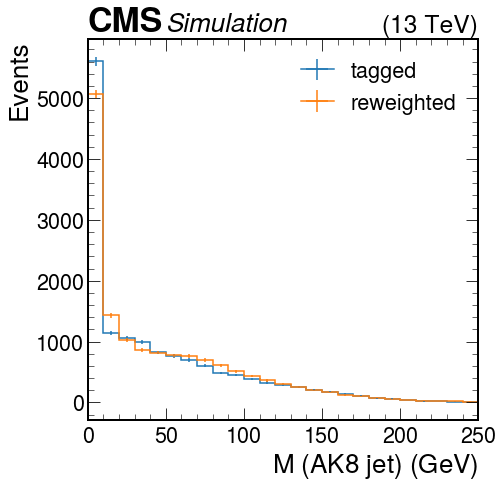
\includegraphics[width=0.6\textwidth]{Chapters/Strategy/tagcheck.png}
\caption{A comparison of the $m_\text{AK8}$ distribution in a Run 2 Z+jets $\to$ $\nu\nu$ sample.}
\label{fig:tagcheck}
\end{figure}

The next set of restrictions on the events is aimed at reducing the prominence of the main backgrounds in the signal region, particularly the multijet background. Jets (either AK8 or AK4) that are closely aligned with the \ptmiss are a sign that the jet momentum is poorly reconstructed in that event, giving rise to the missing momentum. As a result, events are required to have $\Delta\varphi(\text{jets}, \ptvecmiss) > 1$. To further eliminate events with poorly reconstructed jet momenta, events are required to have $\Delta\varphi(\text{AK4 jets}, \ptvecmiss) < 3$. Finally, there is a restriction on jets in a back-to-back configuration, which is a typical sign of multijet production.

As described in \cref{section:2hdma}, under the 2HDM+a model the SM Higgs and the \ptmiss originate from the decay of the pseudoscalar A. $m_\mathrm{A}$ is approximated as

\begin{equation}
    \mt = \sqrt{2\pt(\text{AK8 jets})\ptmiss(1-\cos(\varphi(\text{AK8 jets})-\varphi(\ptvecmiss))}.
    \label{eq:mt}
\end{equation}

This variable is calculated for each AK8 jet, and each event is required to have at least one AK8 jet that has a corresponding \mt of at least $\GeV{600}$.

The baseline event selection is given in \cref{tab:selection}. The relative effectiveness of each selection is shown in \crefrange{fig:metpt}{fig:dphi} where the relevant variable is plotted with each other selection having been applied. Finally, the cumulative effect of the selections is given in \cref{tab:cutflow} which shows the events remaining after each successive selection, split amongst the main background categories and three signals.

\begin{table}
  \centering
  \caption{Summary of the event selection. The requirement that events include at least one h-tagged AK8 means that at least one AK8 jet is required and events are weighted depending on the tagging efficiencies of AK8 jets in the event to mirror the effect of using a Higgs tagger.}
  \begin{tabular}{r|l}
    Observable & Requirement \\
    \hline
    $N_{\text{leptons}}$ & $ = 0$ \\
    \ptmiss & $> \GeV{300}$ \\
    $N_{\text{h-tagged AK8}}$ & $ > 0$ \\
    min $\pt(\text{AK8 jets})$ & $>\GeV{300}$ \\
    $N_{\text{AK4}}$ & $ > 1$ \\
    $\text{min}~ \Delta\varphi(\text{AK8 jets}, \ptvecmiss)$ & $ > 1$ \\
    $\text{min}~ \Delta\varphi(\text{AK4 jets}, \ptvecmiss)$ & 1 -- 3  \\
    $\Delta\varphi(\text{any 2 AK8 jets})$ & $ < 3$ \\
    $\Delta\varphi(\text{any 2 of 4 lead AK4 jets})$ & $ < 3$ \\
    $\text{min}~ \mt(\text{AK8 jets}, \ptvecmiss)$ & $ > \GeV{600}$ \\
  \end{tabular}
  \label{tab:selection}
\end{table}



\begin{figure}[ht]
\centering
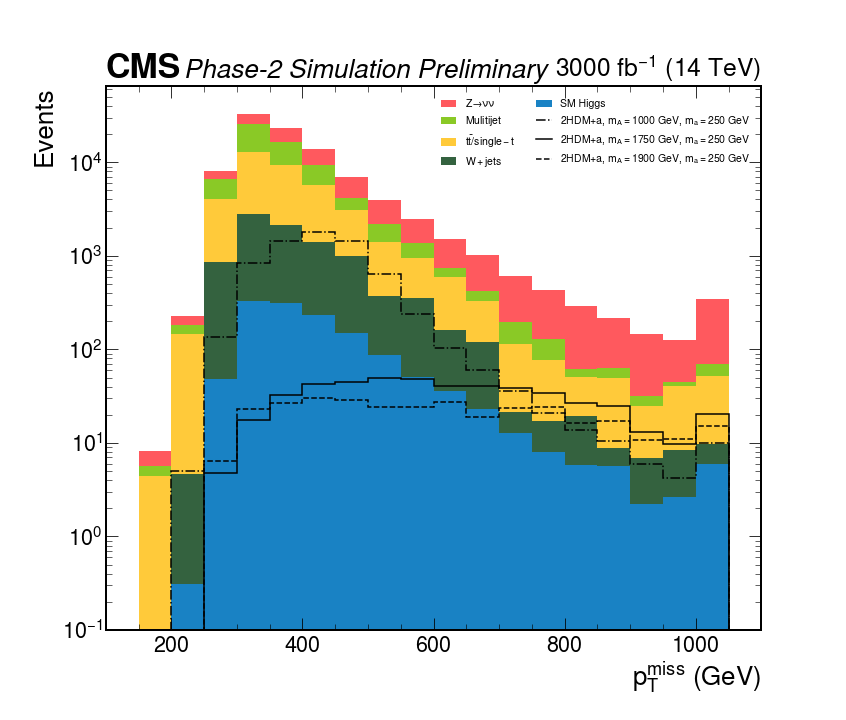
\includegraphics[width=0.845\textwidth]{Chapters/Strategy/selections/met_pt.png}
\caption{The \ptmiss distribution among the backgrounds and the $m_\mathrm{A} =1000$, $1750$, and 
$\GeV{1900}$, $m_\mathrm{a} = \GeV{250}$ signals with each selection except the \ptmiss cut applied.}
\label{fig:metpt}
\end{figure}

\begin{figure}[ht]
\centering
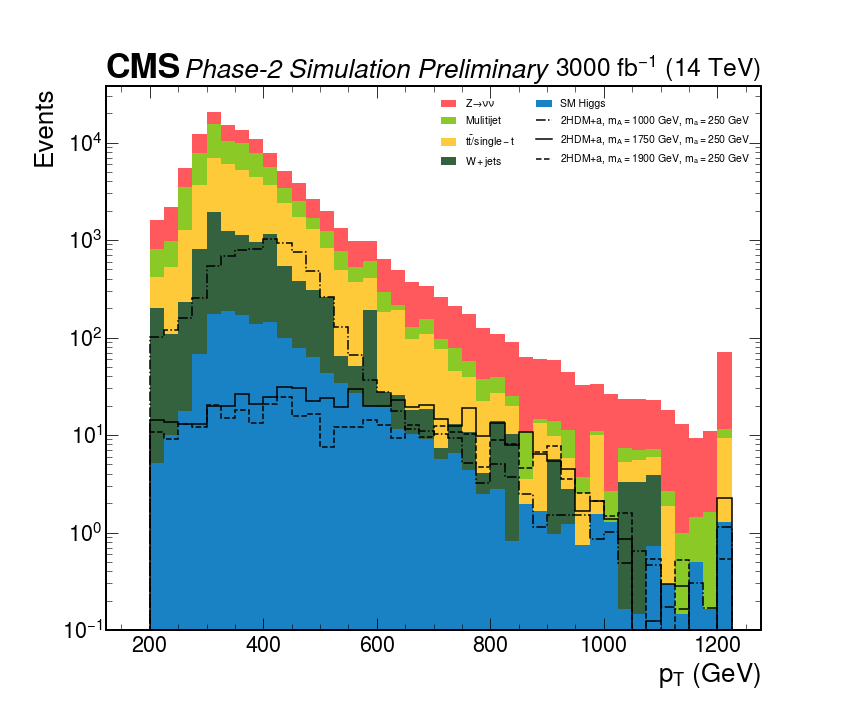
\includegraphics[width=0.845\textwidth]{Chapters/Strategy/selections/min_AK8_pt.png}
\caption{The minimum \pt of the AK8 jets in an event in the backgrounds and the $m_\mathrm{A} =1000$, $1750$, and $\GeV{1900}$, $m_\mathrm{a} = \GeV{250}$ signals with each selection except the min \pt cut applied.}
\label{fig:minak8pt}
\end{figure}

\begin{figure}[ht]
\centering
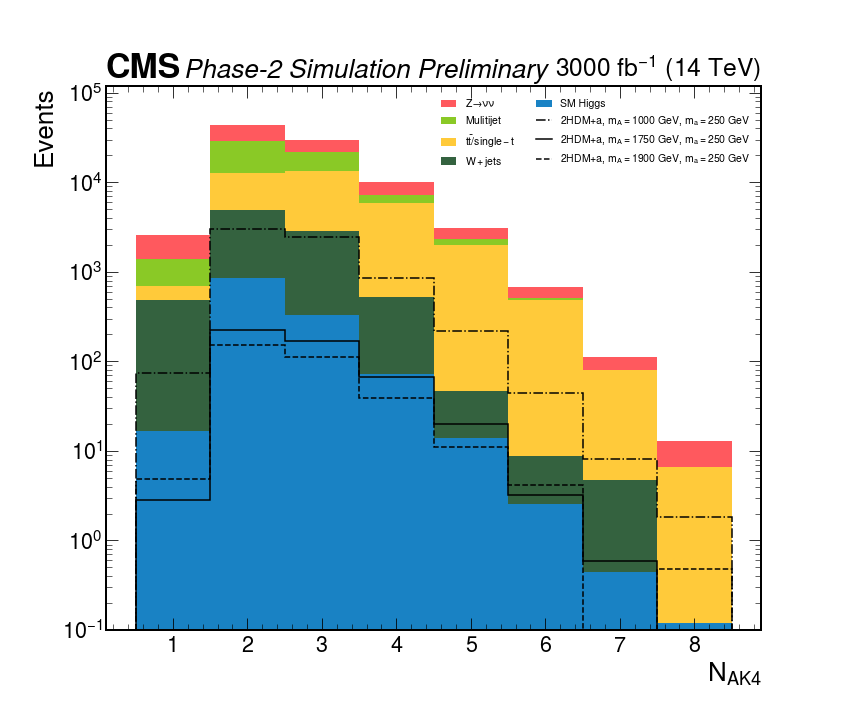
\includegraphics[width=0.845\textwidth]{Chapters/Strategy/selections/n_AK4.png}
\caption{The number of the AK4 jets in each event in the backgrounds and the $m_\mathrm{A} =1000$, $1750$, and $\GeV{1900}$, $m_\mathrm{a} = \GeV{250}$ signals with each selection except the $N_\text{AK4}$ cut applied.}
\label{fig:nak4}
\end{figure}

\begin{figure}[ht]
\centering
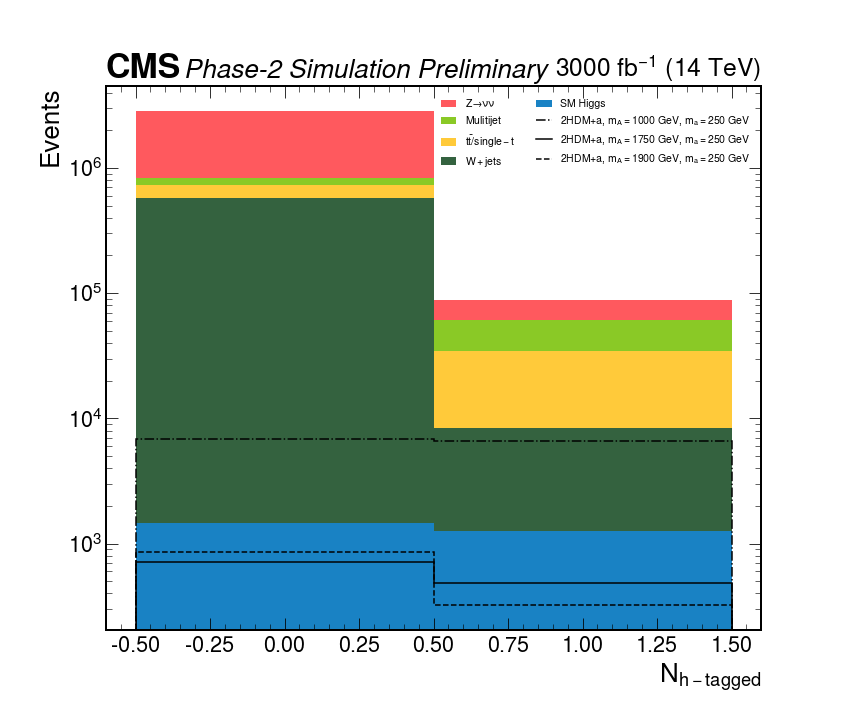
\includegraphics[width=0.845\textwidth]{Chapters/Strategy/selections/NH_weight.png}
\caption{The number of h-tagged jets in the backgrounds and the $m_\mathrm{A} =1000$, $1750$, and $\GeV{1900}$, $m_\mathrm{a} = \GeV{250}$ signals with each selection except the Higgs tagging requirement applied. The Higgs tagging has been done via event weighting, as described above. The right bin is an overflow bin containing all events with one or more h-tagged jets.}
\label{fig:mt}
\end{figure}

\begin{figure}[ht]
    \centering
    
    \begin{subfigure}[b]{0.45\textwidth}
        \centering
        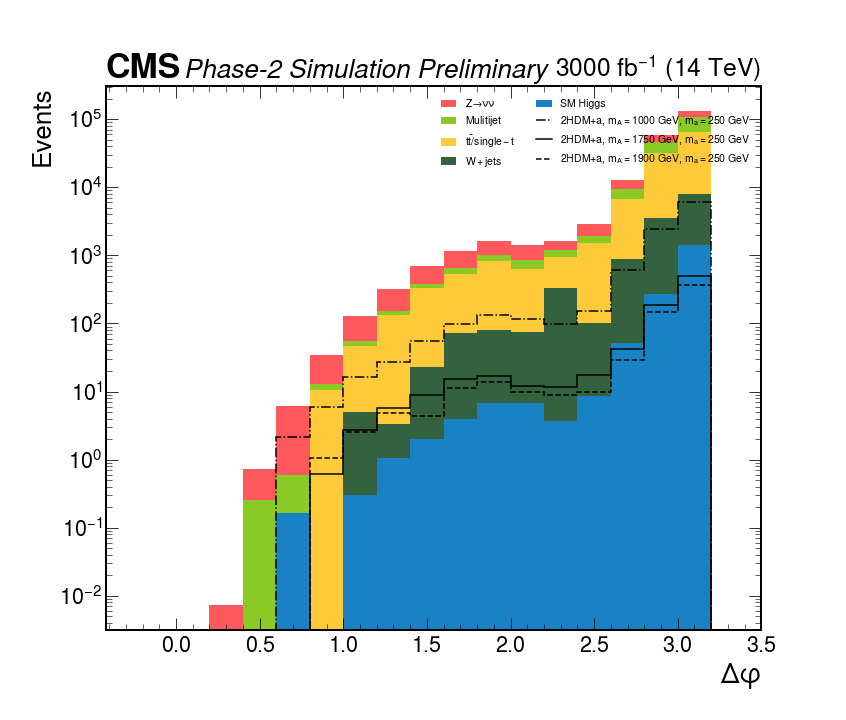
\includegraphics[width=\textwidth]{Chapters/Strategy/selections/dphi_AK8_MET.png}
        \caption{The min $\Delta\varphi(\text{AK8 jets},\ptvecmiss)$ distribution.}
        \label{fig:dphiak8met}
    \end{subfigure}
    \hfill
    \begin{subfigure}[b]{0.45\textwidth}
        \centering
         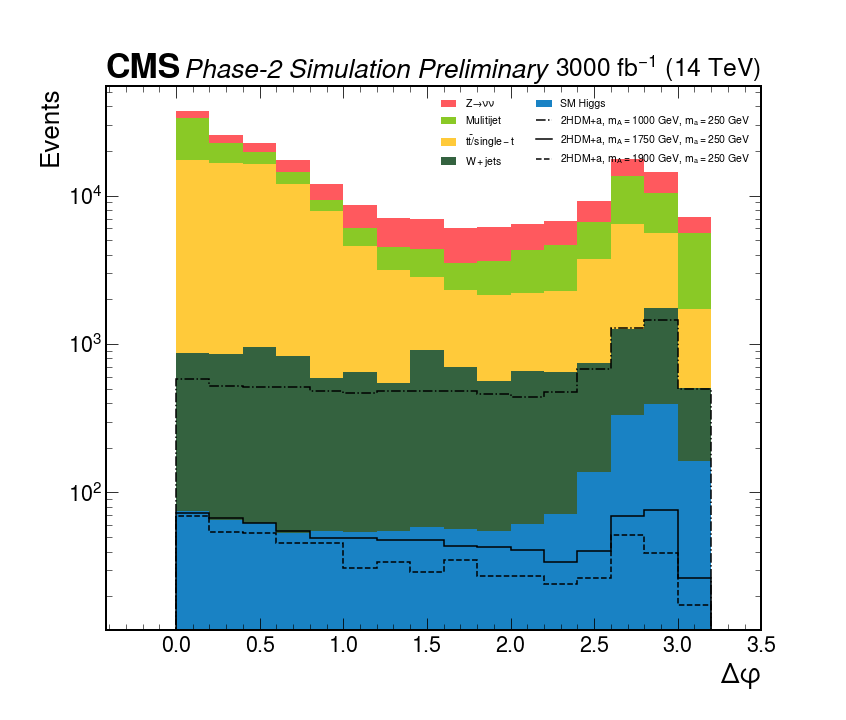
\includegraphics[width=\textwidth]{Chapters/Strategy/selections/dphi_AK4_MET.png}
        \caption{The min $\Delta\varphi(\text{AK4 jets},\ptvecmiss)$ distribution.}
        \label{fig:dphiak4met}
    \end{subfigure}
    
    \begin{subfigure}[b]{0.45\textwidth}
        \centering
        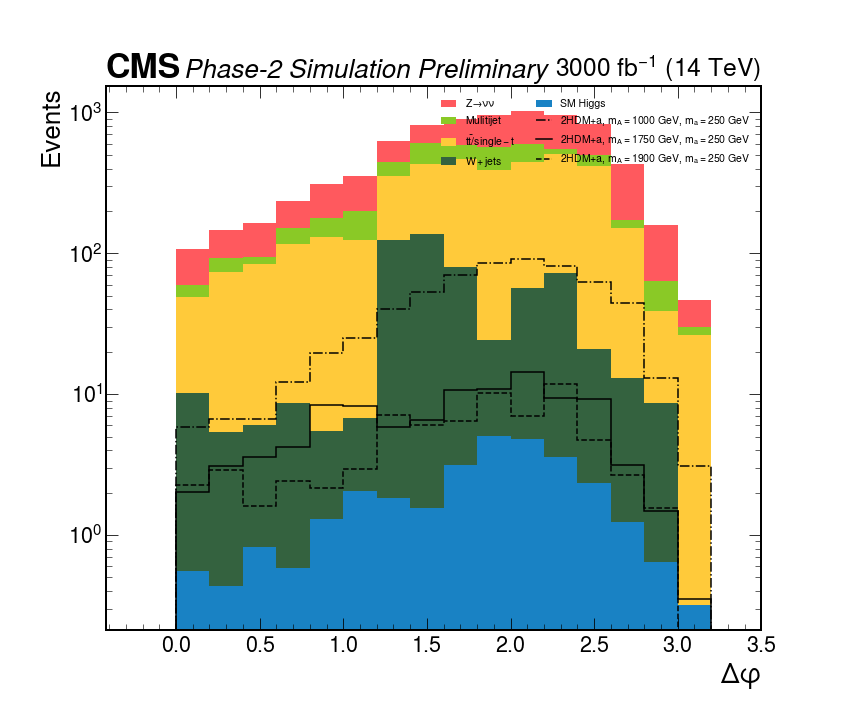
\includegraphics[width=\textwidth]{Chapters/Strategy/selections/AK8_QCD_veto.png}
        \caption{The $\Delta\varphi(\text{any 2 AK8 jets})$ distribution.}
        \label{fig:dphi2ak8}
    \end{subfigure}
    \hfill
    \begin{subfigure}[b]{0.45\textwidth}
        \centering
        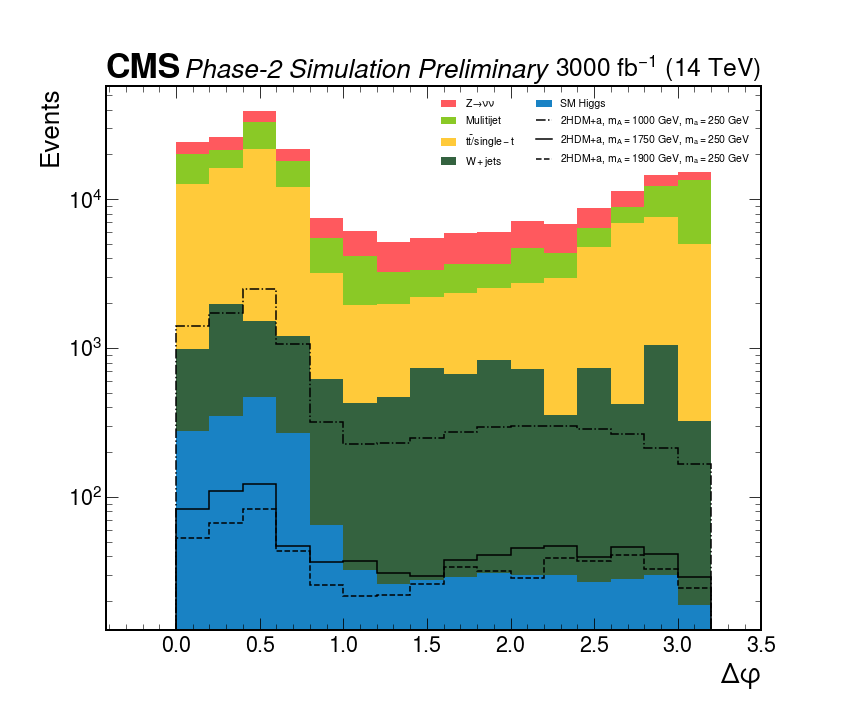
\includegraphics[width=\textwidth]{Chapters/Strategy/selections/AK4_QCD_veto.png}
        \caption{The $\Delta\varphi(\text{any 2 of 4 lead AK4 jets})$ distribution.}
        \label{fig:dphi2o4ak4}
    \end{subfigure}
    \caption{The distributions of the various $\Delta\varphi$ in the backgrounds and the $m_\mathrm{A} =1000$, $1750$, and $\GeV{1900}$, $m_\mathrm{a} = \GeV{250}$ signals with each selection except for any of the $\Delta\varphi$ cuts applied.}
    \label{fig:dphi}
\end{figure}

\begin{sidewaystable}
\centering
\caption{Yields for three chosen signals and the predominant backgrounds.}
\begin{adjustbox}{width=10in}
\begin{tabular}{|c|c|c|c|c|c|c|c|c|}
\hline
 & Z$\to\nu\nu$ & W+jets & Multijet & t$\bar{\mathrm{t}}$/single-t & SM h & $m_\mathrm{A}=\GeV{1000}$, $m_\mathrm{a}=\GeV{250}$ & $m_\mathrm{A}=\GeV{1750}$, $m_\mathrm{a}=\GeV{250}$ & $m_\mathrm{A}=\GeV{1900}$, $m_\mathrm{a}=\GeV{250}$  \\
\hline
Initial                                          & $1226000000\pm40000$ & $214600000000\pm500000$ & $2141000000\pm50000$ & $489500000\pm20000$  & $1929000\pm1000$ & $103100\pm300$ & $188500\pm400$ & $340000\pm600$ \\
$N_\text{leptons} = 0$                           & $1016000000\pm30000$ & $84670000000\pm300000$  & $1457000000\pm40000$ & $101600000\pm10000$  & $701000\pm800$   & $67160\pm260$  & $124500\pm400$ & $224700\pm500$ \\
\ptmiss $> \GeV{300}$                                  & $8339000\pm3000$     & $2595000\pm2000$        & $1103000\pm1000$     & $1288000\pm1000$     & $6647\pm82$      & $28500\pm170$  & $5198\pm72$    & $7374\pm86$    \\
$N_\text{h-tagged AK8} > 0$                      & $114500\pm100$       & $26670\pm80$            & $230800\pm300$       & $226300\pm300$       & $2624\pm35$      & $13140\pm80$   & $1556\pm29$    & $1555\pm28$    \\
min \pt (AK8 jets) $> \GeV{300}$               & $51860\pm90$         & $13380\pm50$            & $126600\pm200$       & $141600\pm200$       & $1811\pm30.$     & $10270\pm70$   & $1066\pm25$    & $983.1\pm22.7$ \\
$N_\text{AK4} > 1$                               & $51860\pm90$         & $13380\pm50$            & $126600\pm200$       & $141600\pm200$       & $1811\pm30$      & $10270\pm70$   & $1066\pm25$    & $983.1\pm22.7$ \\
min $\Delta\varphi$(AK8, \ptmiss) $> 1$          & $47110\pm80$         & $12370\pm50$            & $60630\pm140$        & $97180\pm160$        & $1769\pm30$      & $10050\pm70$   & $847.8\pm21.8$ & $644.5\pm18.0$ \\
$3>\text{min }\Delta\varphi$(AK4, \ptmiss)$>1$   & $29520\pm70$         & $7822\pm39$             & $26900\pm100$        & $27690\pm80$         & $1289\pm25$      & $6891\pm60$    & $505.4\pm17.0$ & $345.8\pm13.8$ \\
$\Delta\varphi(\text{2 AK8 jets}) < 3$           & $29460\pm60$         & $7820\pm39$             & $26850\pm100$        & $27650\pm80$         & $1289\pm25$      & $6882\pm60$    & $504.8\pm17.0$ & $344.9\pm13.8$ \\
$\Delta\varphi(\text{2 of 4 lead AK4 jets}) < 3$ & $28800\pm60$         & $7769\pm39$             & $26640\pm100$        & $27050\pm80$         & $1282\pm25$      & $6795\pm60$    & $496.3\pm16.9$ & $339.8\pm13.7$ \\
min \mt $> \GeV{600}$                          & $27040\pm60$         & $7116\pm37$             & $26180\pm100$        & $26340\pm80$         & $1267\pm25$      & $6618\pm59$    & $483.9\pm16.7$ & $321.4\pm13.3$ \\
\hline
AK8 jet on Higgs mass                            & $5718\pm30$          & $1799\pm20.0$           & $8830\pm60$          & $10360\pm50$         & $884.9\pm21.1$   & $4324\pm48$    & $301.3\pm13.3$ & $188.4\pm10.5$ \\
\hline
\end{tabular}
\end{adjustbox}
\label{tab:cutflow}
\end{sidewaystable}

\chapter{Signal Extraction}
There are several significant SM processes that contribute to the background to the DM signal. 
The largest background process is events where a lepton is not properly reconstructed by the detector, resulting in a final state that passes the lepton vetoes. Background events of this nature are most likely to produce just a single lepton as well as \ptmiss from a neutrino and have several jets, such as semileptonic t$\bar{\mathrm{t}}$ events and W bosons produced in association with initial state jets. Examples of such processes can be seen in \cref{fig:w+jets,fig:ttbar}.  
The second largest background process is events where a Z boson is produced in association with jets. The Z then decays into two neutrinos, which has a branching ratio of roughly $\text{BR(Z}\to\nu\nu) = 0.2$~\cite{Zyla:2020zbs}. The presence of the neutrinos gives the event high \ptmiss, while the initial-state jets can pass the various cuts based on jet kinematics. A representative Feynman diagram of this process is shown in \cref{fig:z+jets}.
The next largest background process is multijet production.
The smallest relevant background are other processes where a Higgs boson is produced, such as the Zh and Wh processes.

\begin{figure}[ht]
\centering
     \begin{subfigure}[b]{0.25\textwidth}
         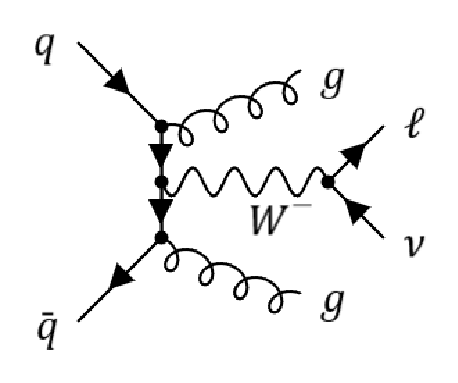
\includegraphics[width=\textwidth]{Chapters/Signal_Extraction/w+jets.pdf}
         \caption{A W boson decaying to a neutrino and a lepton in association with two partons.}
         \label{fig:w+jets}
     \end{subfigure}
     \begin{subfigure}[b]{0.25\textwidth}
         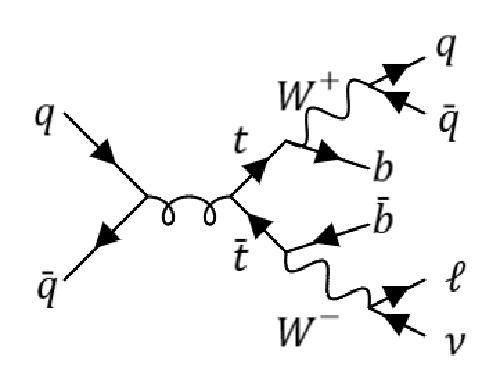
\includegraphics[width=\textwidth]{Chapters/Signal_Extraction/ttbar.pdf}
         \caption{\raggedright A t$\bar{\mathrm{t}}$ process where one W boson decays leptonically and the other decays hadronically.}
         \label{fig:ttbar}
     \end{subfigure}
    \begin{subfigure}[b]{0.25\textwidth}
         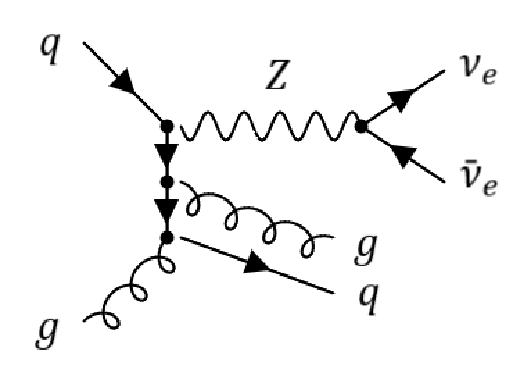
\includegraphics[width=\textwidth]{Chapters/Signal_Extraction/z+jets.pdf}
         \caption{A Z boson decaying to two neutrinos in association with two partons.}
         \label{fig:z+jets}
     \end{subfigure}
\caption{Feynman diagrams representing several processes that can contribute to the background of a 2HDM+a signal.}
\end{figure}

To estimate the level of background events in the final selection, it is useful to identify properties that are significantly different between the background and signal events. One useful variable for doing so is the mass of the highest-momentum AK8 jet in the event, referred to as $m_{\text{AK8}}$. 
Events resulting from multijet processes and Z or W boson production in association with initial state jets are expected to have low-mass jets, as most of these jets come from high-momentum gluons. 
However, in events where the decay of a heavy object such as a W boson or top quark is reconstructed as an AK8 jet, that jet will have a mass around $\GeV{80}$ and $\GeV{170}$, respectively. 
Finally, events from the signal or from the Higgs background processes will have an AK8 jet with a mass around that of the SM Higgs, $\GeV{125}$. These relative populations can be seen in \cref{fig:ak8massshape}. 
This suggests dividing events into 4 $m_\text{AK8}$ bins: $0\text{--}\GeV{50}$, $50\text{--}\GeV{100}$, $100\text{--}\GeV{150}$, and $>\GeV{150}$. Although the background estimations in this analysis are done using simulated events, adding mass sidebands allows these estimates to be constrained using a data-driven background estimation for an analysis done at the HL-LHC.

\begin{figure}[ht]
\centering
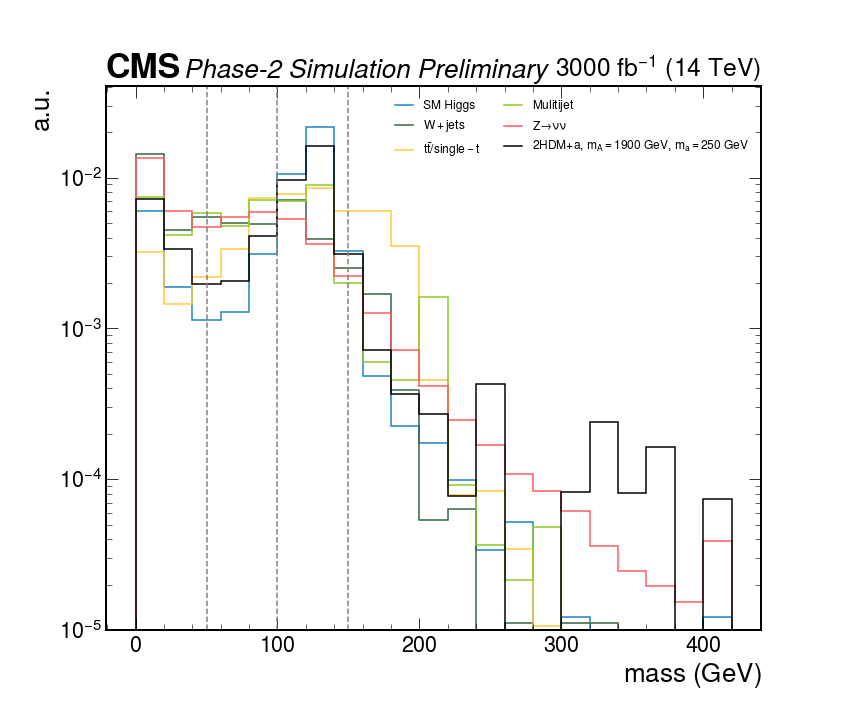
\includegraphics[width=0.845\textwidth]{Chapters/Signal_Extraction/shape_AK8_sdmass.png}
\caption{The $m_\text{AK8}$ distribution in the final selection. Shown here are the main backgrounds and the $m_\mathrm{A} = \GeV{1900}$, $m_\mathrm{a} = \GeV{250}$ signal. The histograms are normalized to an integral of 1.}
\label{fig:ak8massshape}
\end{figure}

In addition to $m_\text{AK8}$, there is a significant difference between the signal and background in the distribution of the minimum \mt of the AK8 jet-\ptmiss system, as can be seen in \cref{fig:mtshape}. The signal has a much more prominent tail, while the background peaks far earlier. 10 even \mt bins are selected between $600$ and $\GeV{2400}$ , with the last bin containing all events with \mt greater than $\GeV{2400}$. Multiple \mt bins are chosen in order to cover the wide range of masses of the pseudoscalar A that I examine in this thesis.

\begin{figure}[ht]
    \centering
    \begin{subfigure}[b]{\textwidth}
        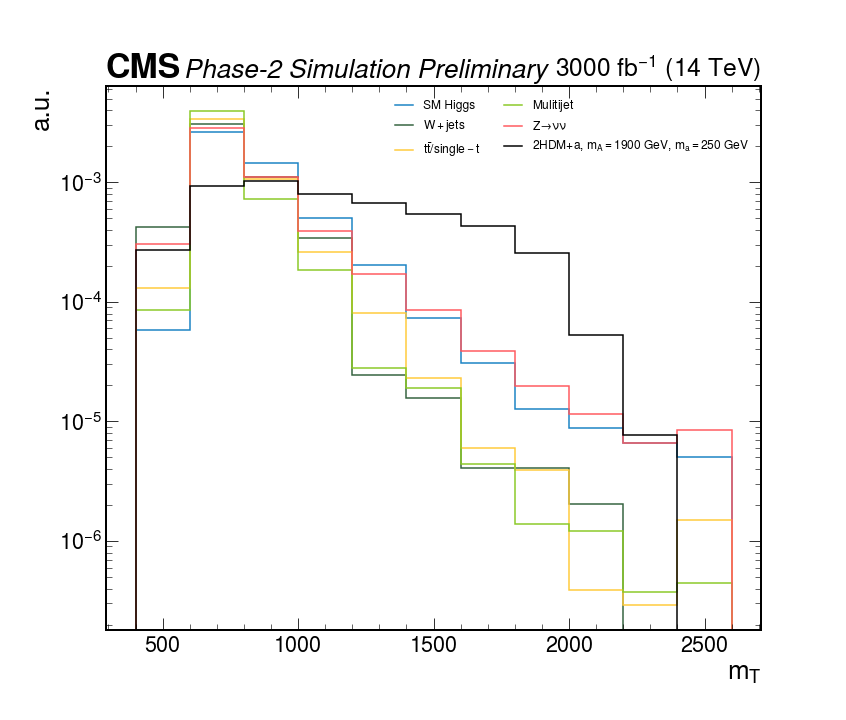
\includegraphics[width=0.845\textwidth]{Chapters/Signal_Extraction/shape_MT_backgrounds.png}
    \end{subfigure}
    \begin{subfigure}[b]{\textwidth}
        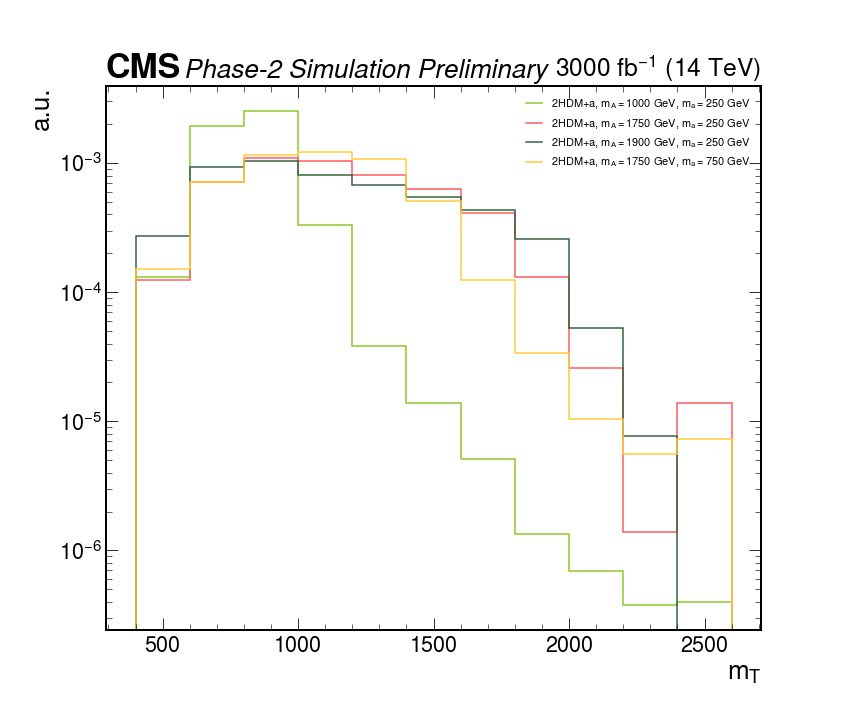
\includegraphics[width=0.845\textwidth]{Chapters/Signal_Extraction/shape_MT_signals.png}
    \end{subfigure}
\caption{The \mt distribution in the final selection. Shown in the upper plot are the main backgrounds against the $m_\mathrm{A} = \GeV{1900}$, $m_\mathrm{a} = \GeV{250}$  signal. The lower plot compares the $m_\mathrm{A} =1000$, $1750$, $\GeV{1900}$, $m_\mathrm{a} = \GeV{250}$ and $m_\mathrm{A} = \GeV{1750}$, $m_\mathrm{a} = \GeV{750}$ signals. The histograms are normalized to an integral of 1.}
\label{fig:mtshape}
\end{figure}

A histogram of the yields of the main backgrounds and two representative signal points is given in \cref{fig:srbins} showing the contribution of the signal and backgrounds in each bin, as well as the size of the post-fit uncertainties in each bin.

\begin{figure}[ht]
    \centering
    \begin{subfigure}[b]{\textwidth}
        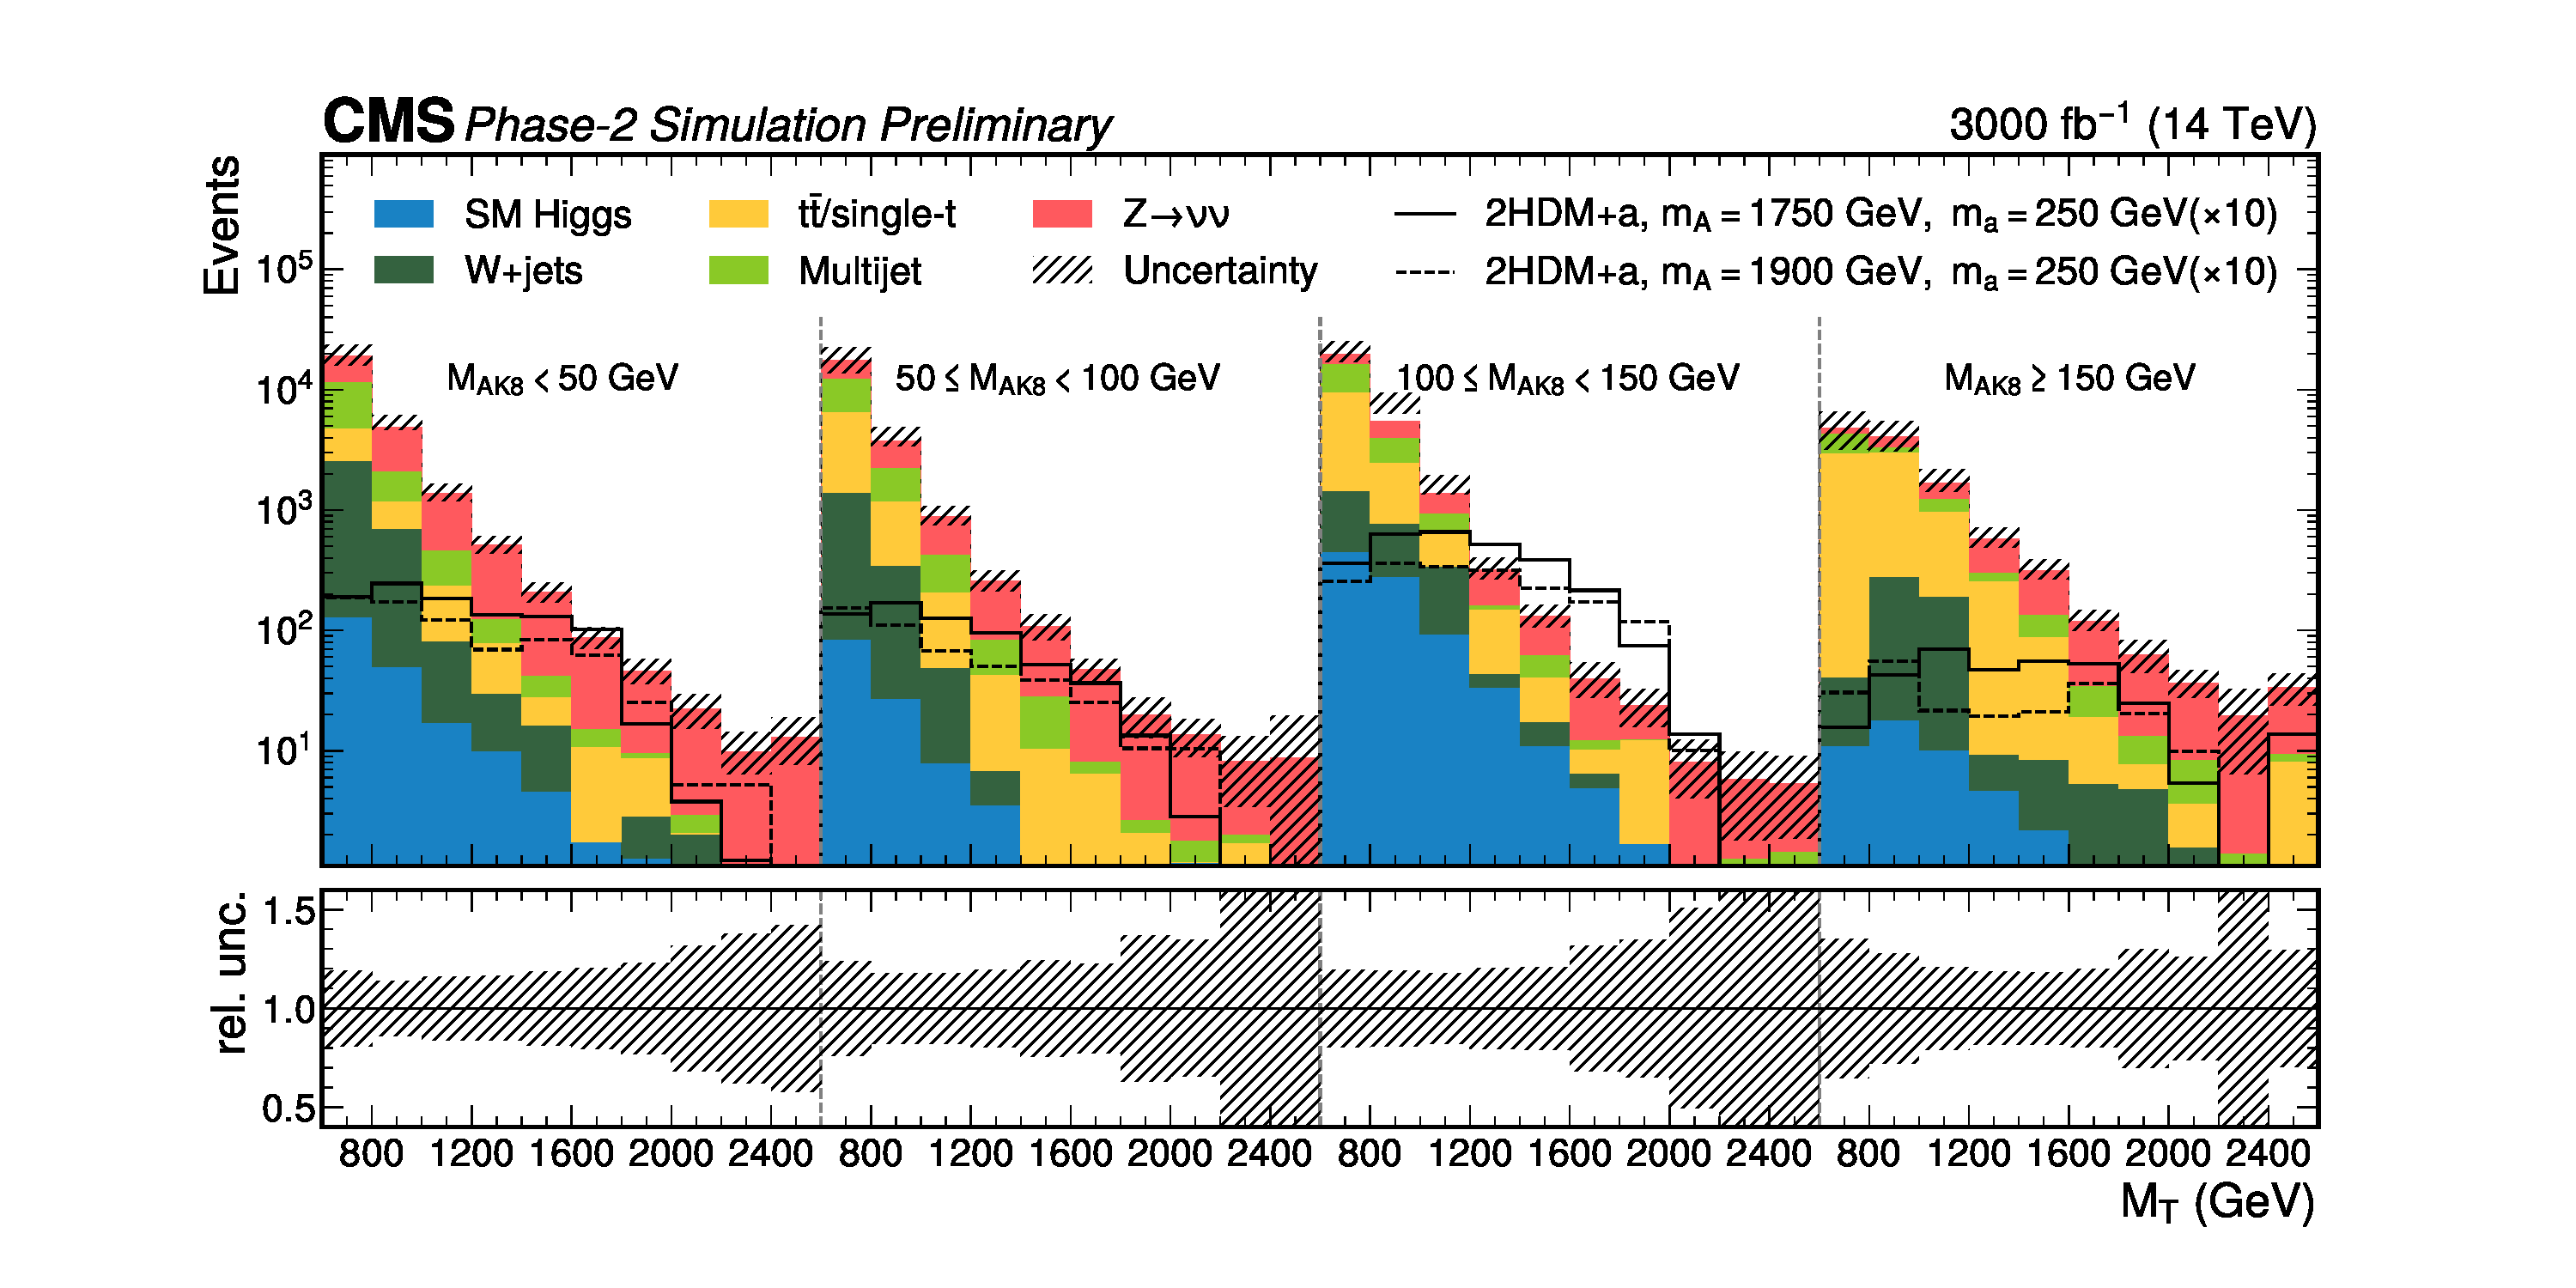
\includegraphics[width=\textwidth]{Chapters/Signal_Extraction/prefit_sr.pdf}
    \end{subfigure}
    \begin{subfigure}[b]{\textwidth}
        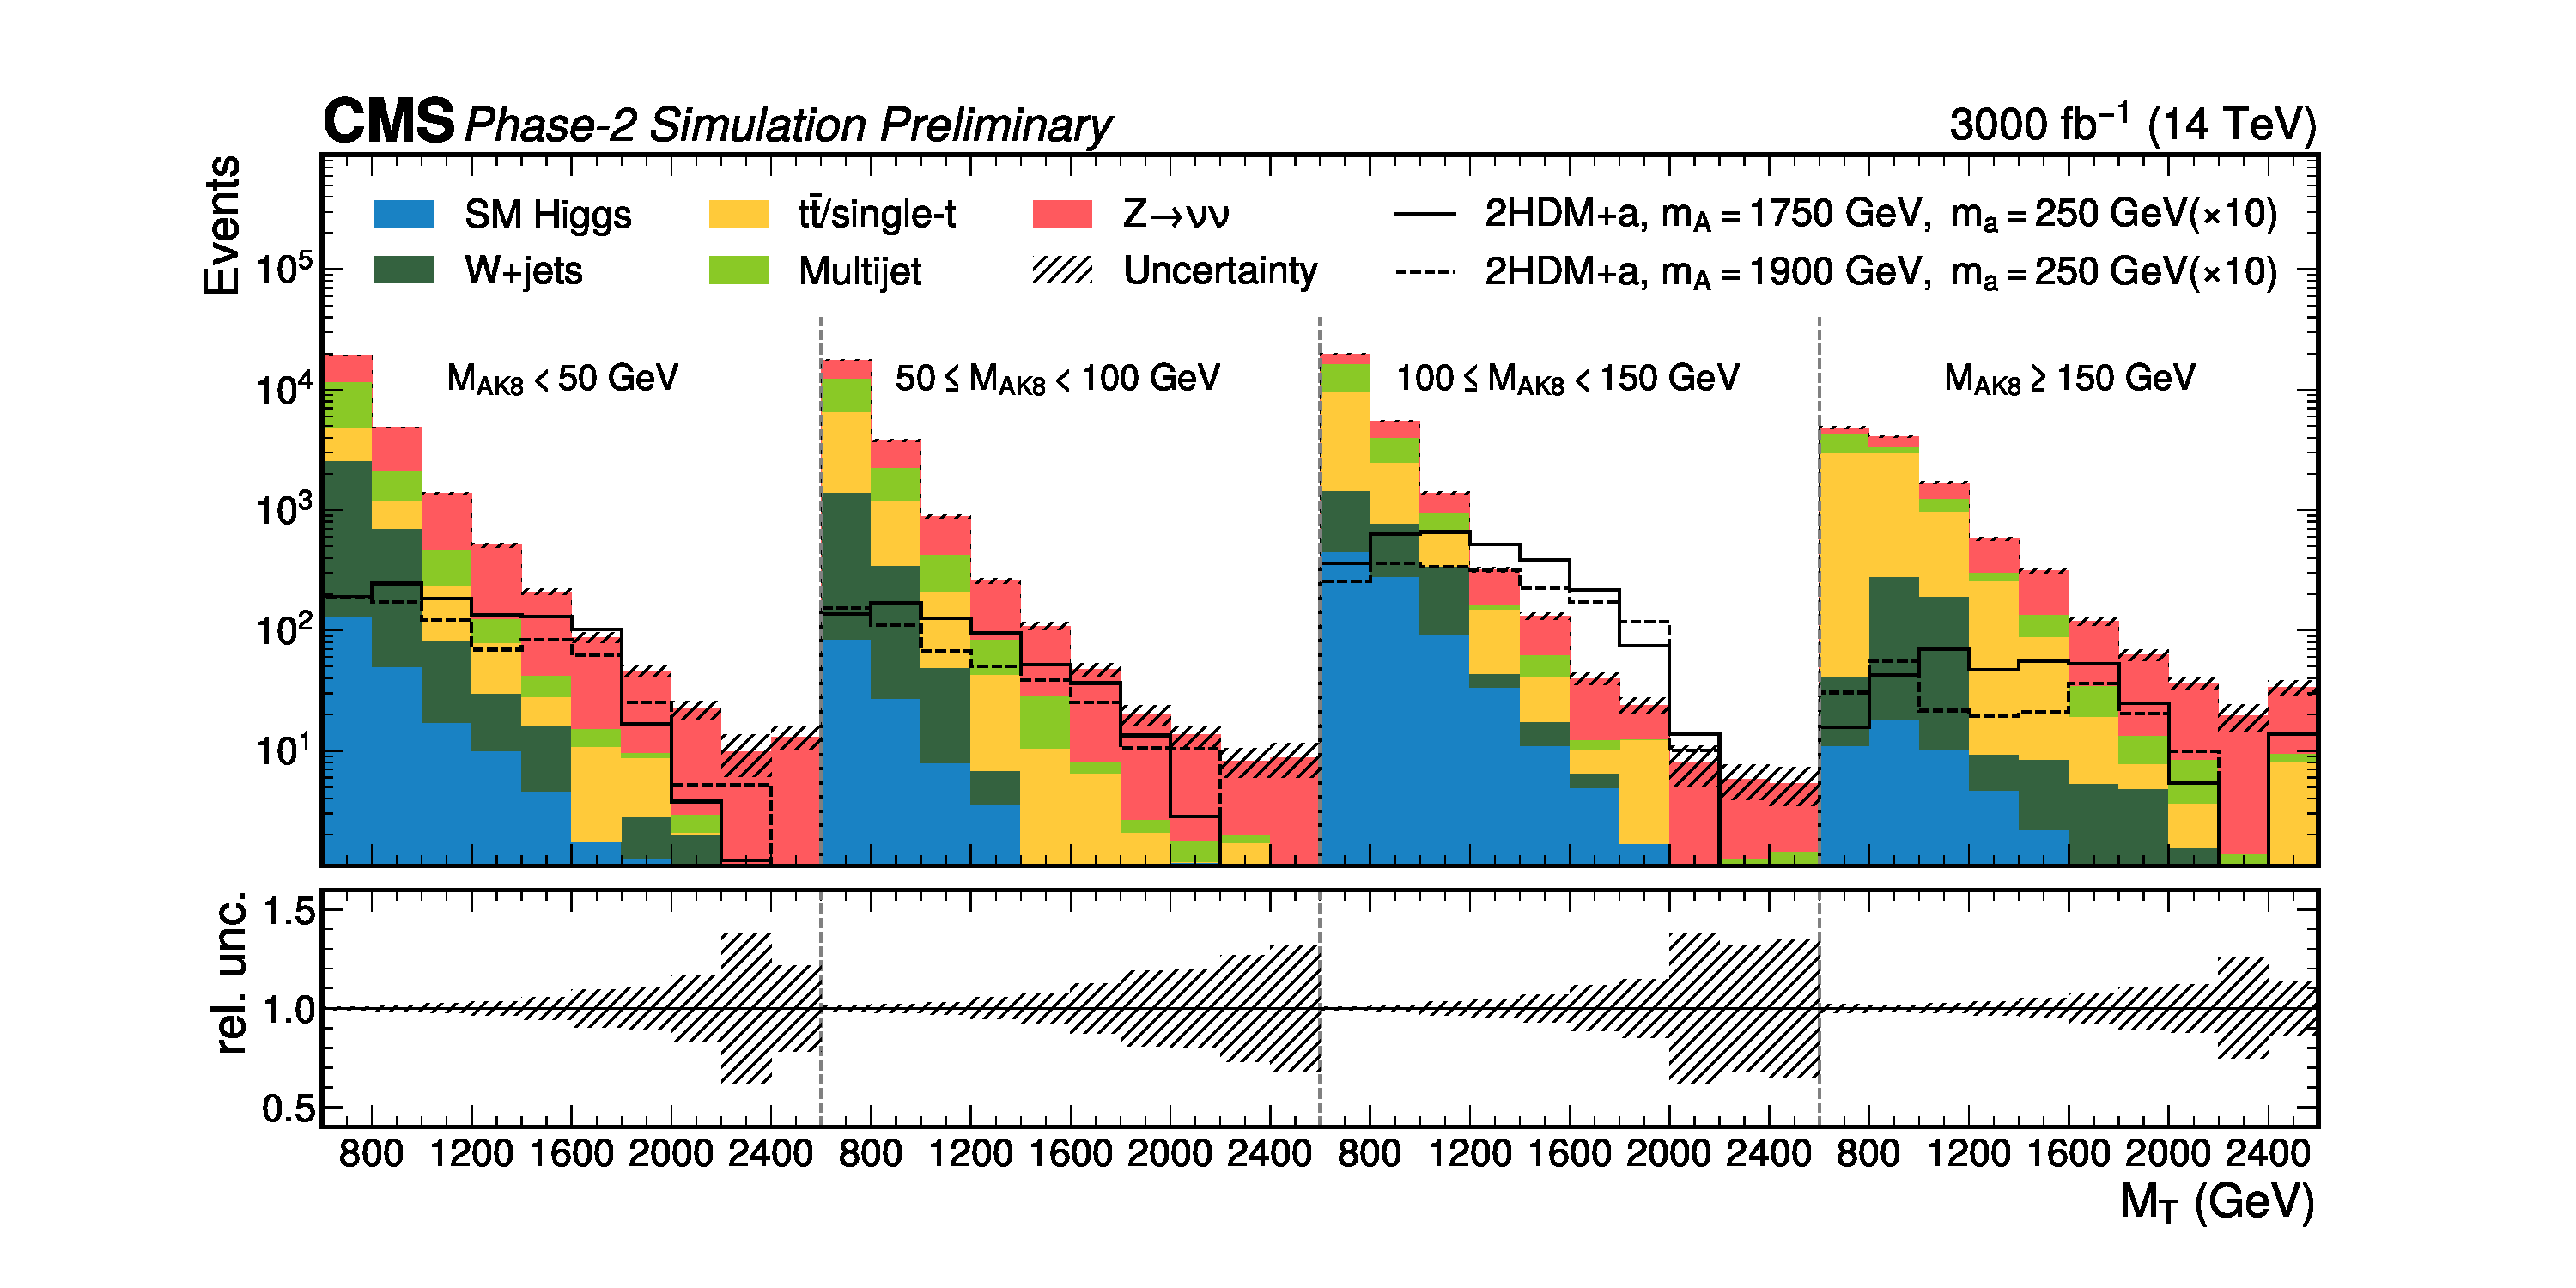
\includegraphics[width=\textwidth]{Chapters/Signal_Extraction/postfit_sr.pdf}
    \end{subfigure}
    \caption{The yield of the main backgrounds and two 2HDM+a signals with $m_\mathrm{A} = \GeV{1750}$, $m_\mathrm{a} = 250$, $\GeV{750}$. The signal is scaled tenfold for the purpose of contrasting the shape with the backgrounds. The total pre- and post-fit uncertainties in each bin are given by the shading, with the lower plot showing the relative uncertainty.}
    \label{fig:srbins}
\end{figure}
\chapter{Systematic Uncertainties}
The signal and background processes are affected by a variety of systematic effects that contribute to an overall uncertainty in the yields of each. Understanding these systematic uncertainties is important not only for undertaking a statistical analysis of the results, but also to ensure that no systematic is overly constrained when they are fit during the limit calculation.

The largest systematic uncertainty impacting this search is the uncertainty in the jet mass scale and resolution. By comparing the jet mass resolution using the \textsc{Delphes} framework to the resolution in Run 2, as is done in \cref{fig:jmr}, it is apparent that the former is likely overly optimistic of the eventual Phase-2 resolution. To account for the uncertainty in the eventual resolution and scale, the AK8 jet mass distribution is smeared and shifted by a Gaussian distribution, which is good approximation for the Run 2 resolution near $m_\mathrm{h}$. This new distribution is then used to calculate signal region yields which are compared to the original yields to obtain a nuisance as shown in \cref{eq:nuis}.

\begin{figure}[ht]
\centering
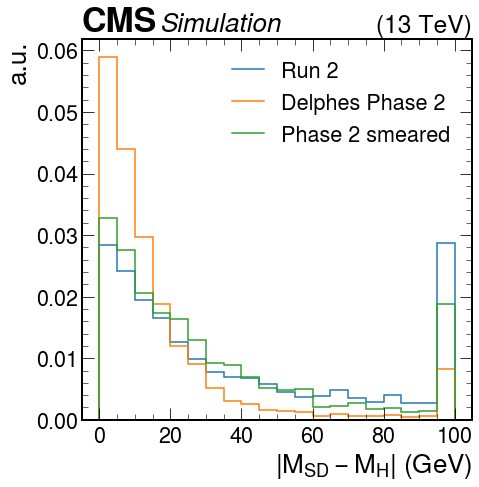
\includegraphics[width=0.6\textwidth]{Chapters/Systematics/jmr.png}
\caption{The absolute difference between the AK8 jet soft drop mass and $m_\mathrm{h}$. Plotted are t$\bar{\mathrm{t}}$h samples from Run 2, \textsc{Delphes}, and \textsc{Delphes} with the Gaussian smearing applied.}
\label{fig:jmr}
\end{figure}

\begin{equation}
    \text{nuisance}_{\pm} = 1\pm\frac{\text{new yield}-\text{old yield}}{\text{old yield}}
    \label{eq:nuis}
\end{equation}

The jet resolution and scale uncertainties are large, but do not employ a more complicated correlation scheme that would likely be used at the HL-LHC. In order to not overly constrain the large uncertainty, flat, partially correlated uncertainties on the mass and \mt binning are assigned. This is done by having an uncertainty correlated in the mass bins, but uncorrelated in the \mt bins and having an uncertainty correlated in the \mt bins, but uncorrelated in the mass bins.

The next largest group of systematic uncertainties come from the theoretical uncertainties affecting the cross-sections of the signals and backgrounds. Uncertainties in the values of $\alpha_S$ are calculated by varying the value of $\alpha_S$ in the simulated events, then comparing the new yields after those variations to the previous yields, similar to the \cref{eq:nuis}. Additional systematic uncertainties come from varying the choice of PDF as well as the factorization scale $\mu_F$ and the renormalization scale $\mu_R$ of the PDF~\cite{Buckley_2015}.

The next largest group of systematic uncertainties comes from uncertainties on the tagging and mistagging rate of the h $\to$ b$\bar{\mathrm{b}}$ tagger. The tag and mistag rates are varied up and down by 10\%. The nuisances are then calculated by taking the difference between the yields when the rates are varied up and down and dividing by the central yields.

The next most prominent systematic uncertainty is the jet energy scale. The uncertainty due to this systematic factor is calculated similarly to the jet mass scale. The jet energies are varied by corrections to the jet energy scale. These corrections are propagated to the \ptmiss. The nuisances are then calculated by taking the difference between the yields when the energies are varied up and down and dividing by the central yields.

Finally, a flat systematic uncertainty of 1\% has been assigned as the uncertainty of the integrated luminosity according to the prescription in~\cite{CMS-PAS-FTR-16-002}. A summary of the systematic uncertainties is given in \cref{tab:systematics}. 

The effects of the small size of the events in the \textsc{Delphes} samples have not been included in this search. However, to avoid an overly aggressive assumption of the uncertainty in the yields, a statistical uncertainty is assigned by taking the square root of the yields for each process in each bin.

\begin{table}
    \center
    \caption{Summary of the effect of the systematic uncertainties used in this analysis on the yields.}
    \begin{adjustbox}{width=\textwidth}
    \begin{tabular}{|l|c|c|c|c|c|c|}
    \hline
	Systematic Uncertainty    & Signal    & t$\bar{\mathrm{t}}$/single-t & W+jets  & Multijet & Z+jets  & SM Higgs   \\ \hline
	Luminosity                & 1\%       & 1\%             & 1\%      & 1\%      & 1\%      & 1\%      \\
	Inclusive cross-section   & -        & 25\%            & -       & 50\%     & -       & -       \\
    JES                       & $<10\%$   & $<10\%$         & $<10\%$  & $<15\%$  & $<11\%$  & $<7\%$   \\
    JMS/JMR                   & $<11\%$   & $<15\%$         & $<10\%$  & $<39\%$  & $<9\%$   & $<25\%$  \\
	JMR mass-uncorrelated       & 6\%       & 6\%             & 6\%      & 6\%      & 6\%      & 6\%      \\
	JMR \mt-uncorrelated        & 4--8\%   & 4--8\%         & 4--8\%  & 4--8\%  & 4--8\%  & 4--8\%  \\
	Higgs tagging               & 10\%      & -             & -       & -      & -       & 10\%     \\
	Higgs mistagging            & $<1\%$    & $<10\%$         & $<10\%$  & $<10\%$  & $<7\%$   & $<1\%$   \\
	PDF			            & 1--6\%   & -              & 1\%-6\%  & -       & 1--18\% & 2--21\% \\
	$\alpha_{\text{S}}$                & $<4\%$    & -              & 1--8\%  & -       & 2--9\%  & $<2\%$   \\
	$\mu_{\text{F}}$ and $\mu_{\text{R}}$       & 21--37\% & -              & 9--22\% & -       & 9--23\% & $<32\%$  \\
	\hline
    \end{tabular}
    \end{adjustbox}
    \label{tab:systematics}
\end{table}


Initially, the main source of uncertainty in each bin comes from the systematic uncertainties, with the jet mass resolution and scale uncertainty contributing the largest amount. However, the systematic uncertainties become constrained during the fit. This can be seen in \cref{fig:srbins}, where after fitting the main source of uncertainty appears to be the statistical uncertainty because it grows in relative strength as the number of events in the bin decreases. As a result, \cref{fig:impacts} shows that the uncertainty in jet mass scale and resolution becomes quite constrained, with some other initially large uncertainties such as the uncertainty in choice of PDF and the multijet production cross-section also being somewhat constrained. This is to be expected, considering that I am partially binning in jet mass and because the uncertainty was so large to begin with.

\begin{figure}[ht]
    \centering
    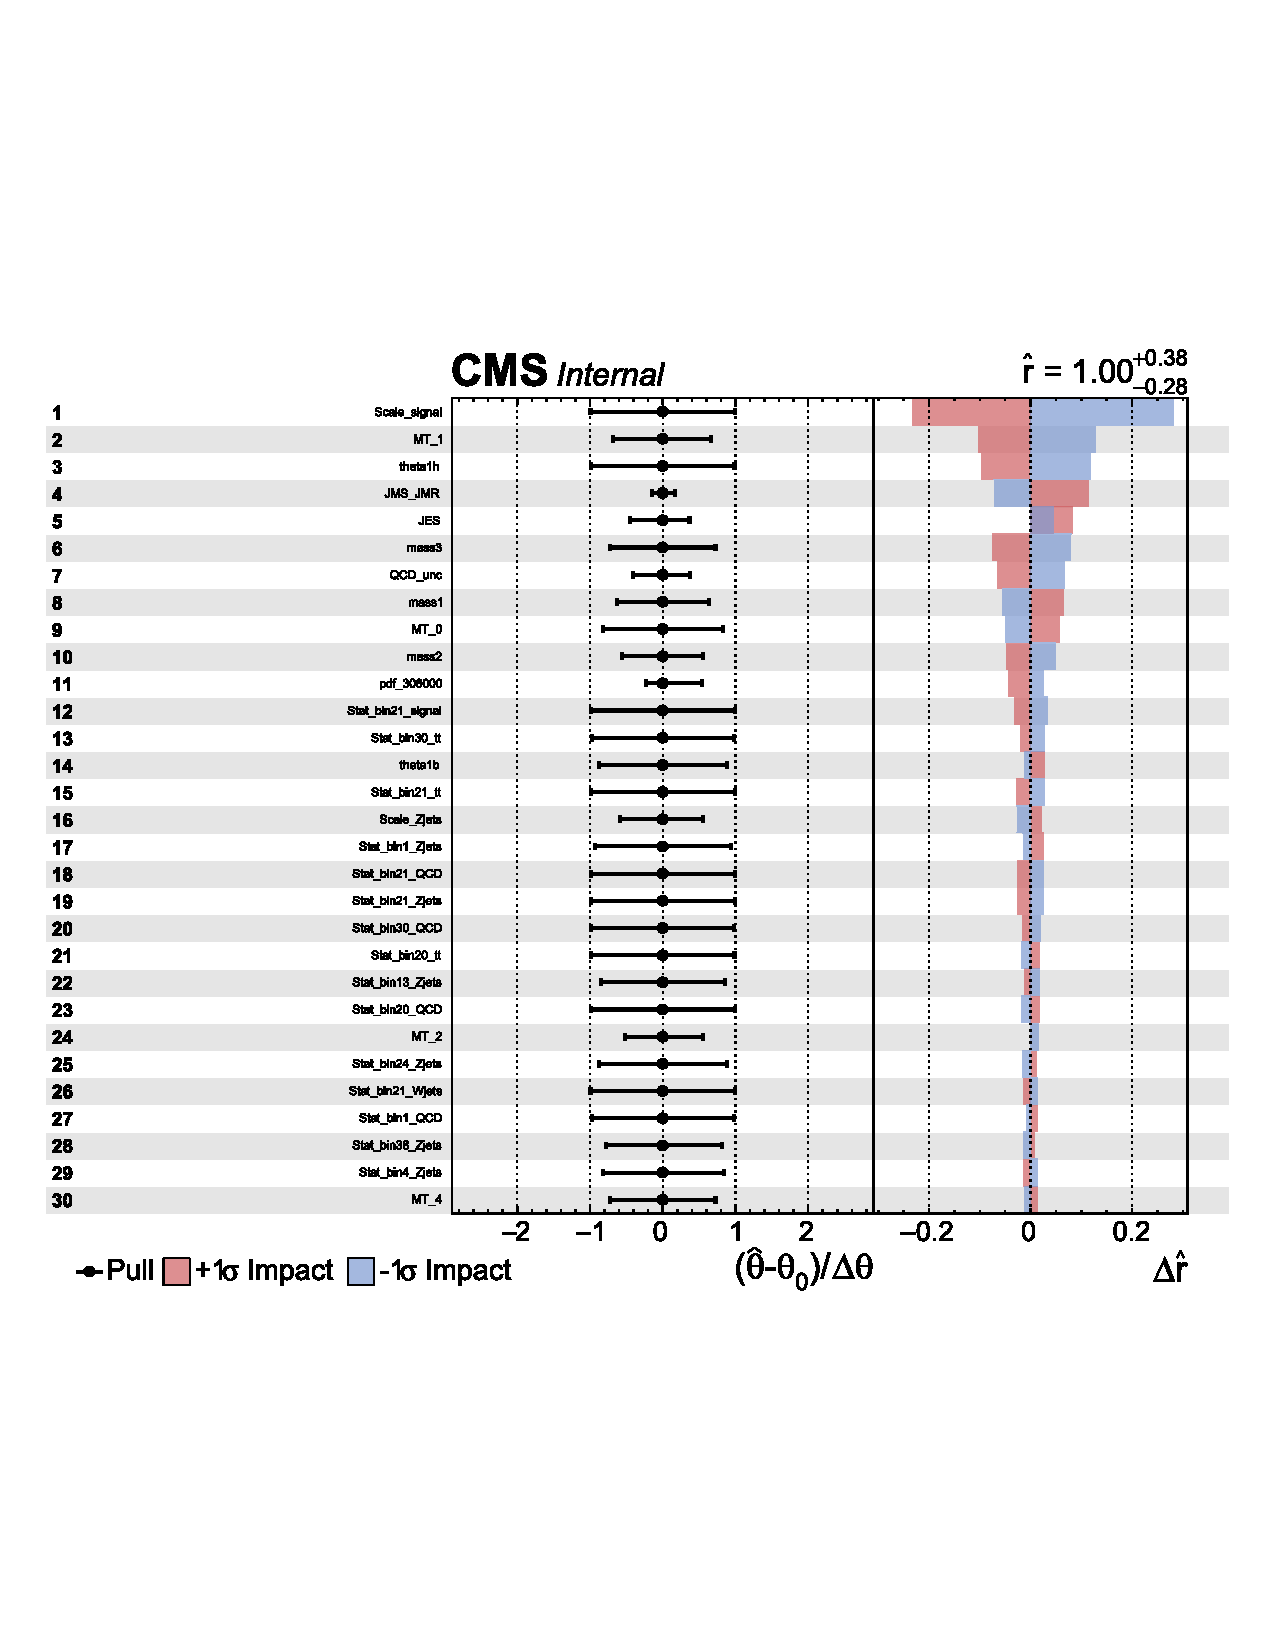
\includegraphics[width=0.9\textwidth]{Chapters/Systematics/impacts_both_sidebands_pg1.pdf}
    \caption{The impacts and pulls of the uncertainties in this search.}
    \label{fig:impacts}
\end{figure}
\chapter{Results and Conclusions}
\section{Results}
In order to derive expected upper limits on the signal strength of the 2HDM+a samples, the likelihood function in \cref{eq:likelihood} is calculated by taking the product of the Poisson probability of the expectation value in each bin. Nuisances are calculated in each bin from the systematic uncertainties using a log-normal distribution.
\begin{equation}
    L(\mu, \boldsymbol{\theta}) = \prod_{j=1}^N\frac{(\mu s_j+b_j)^{n_j}}{n_j!}e^{-(\mu s_j+b_j)}\prod_{k=1}^M\frac{(u_k)^{m_j}}{m_j!}e^{-(u_k)}
    \label{eq:likelihood}
\end{equation}
Here, $s_j$ and $b_j$ are the mean contributions from the signal and background in the bin $j$, which is one of the $m_\text{AK8} = 100\text{--}\GeV{150}$ bins with a number of entries $n_j$. $u_k$ is the mean contribution from the other signal regions $k$ with number of entries $m_k$, which are used to get a handle on the backgrounds in the thesis. In general, these expectation values are dependent on some combination of the nuisances, denoted $\boldsymbol{\theta}$.
The profile likelihood ratio is then calculated by taking the ratio
\begin{equation}
    \frac{L(\mu=1, \boldsymbol{\hat{\hat{\theta}}})}{L(\mu=0, \boldsymbol{\hat{\hat{\theta}}})},
    \label{eq:ratio}
\end{equation}
where $\boldsymbol{\hat{\hat{\theta}}}$ is the value of $\boldsymbol{\theta}$ that maximizes $L$ for the given $\mu$.
Using the asymptotic approximation~\cite{Cowan_2011} for the test statistic described in~\cref{eq:q}, p-values for the hypotheses $\mu=1$ and $\mu=0$ were calculated using~\cref{eq:psb,eq:pb}, respectively. Here, $\sigma_{s+b}$ and $\sigma_{b}$ are the standard deviations of $q$ for the $\mu=1$ and $\mu=0$ hypotheses, respectively, which can be calculated from a covariance of $\mu$ and $\boldsymbol{\theta}$. 
\begin{equation}
    q = -2\ln\frac{L(\mu=1, \boldsymbol{\hat{\hat{\theta}}})}{L(\mu=0, \boldsymbol{\hat{\hat{\theta}}})}
    \label{eq:q}
\end{equation}
\begin{equation}
    p_{s+b} =  1 - \Phi\bigg(\frac{q_\text{obs}+\frac{1}{\sigma^2_{s+b}}}{2/\sigma_{s+b}}\bigg)
    \label{eq:psb}
\end{equation}

\begin{equation}
    p_{b} =  1 - \Phi\bigg(\frac{q_\text{obs}-\frac{1}{\sigma^2_{b}}}{2/\sigma_{b}}\bigg)
    \label{eq:pb}
\end{equation}
The significance is calculated by transforming $1-p_{s+b}$ to the respective quantile that value falls into.
Expected upper limits were calculated using the $CL_s$ test described in~\cite{Junk_1999, Read_2002}. A value for $\mu$ is determined to be the upper limit if it is the largest value for which the ratio $CL_s$, given in \cref{eq:cls}, is equal to 0.05, giving a 95\% $CL_s$ upper limit. 

\begin{equation}
    CL_s = \frac{p_{s+b}}{1-p_{b}}
    \label{eq:cls}
\end{equation}

These results were compared to those in \cite{cms:hbb2019} by applying the baseline selections to the events with an additional requirement that the mass of the highest-momentum AK8 jet be within $\GeV{25}$ of $m_\mathrm{h}$. A likelihood function is then calculated by binning events in \ptmiss in a manner similar to the analysis of the 2016 Run 2 dataset. The expected limits were within 10\% of the previous results for the 2HDM+a signal with $m_\mathrm{A} = \GeV{1000}$, $m_\mathrm{a} = \GeV{150}$. This level of agreement is reasonable considering the changes in process cross-section due to the difference in beam energy, which is demonstrated for the given signal in \cref{tab:sxsec}. In addition, there were differences in the background yields from the differences in object reconstruction and event selection.

\begin{table}
    \small
    \centering
    \caption{Cross-sections of the 2HDM+a signal for the $m_\mathrm{A} = 1000$ GeV, $m_\mathrm{a} = 150$ GeV mass point as a function of the beam energy.}
    \begin{tabular}{|c|c|c|}
        \hline
        Signal & cross-section (pb) & CoM Energy \\
        b$\bar{\mathrm{b}}$ $\to$ A, $m_\mathrm{A} = 1500$ GeV, $m_\mathrm{a} = 150$ GeV  &   $0.0004232 \pm 0.000001942$ & 13 TeV \\
        gg $\to$ A, $m_\mathrm{A} = 1500$ GeV, $m_\mathrm{a} = 150$ GeV  &          $0.03943 \pm 0.0001792$ & 13 TeV \\
        b$\bar{\mathrm{b}}$ $\to$ A, $m_\mathrm{A} = 1500$ GeV, $m_\mathrm{a} = 150$ GeV  &   $0.0005006 \pm 0.000004345$ & 14 TeV \\
        gg $\to$ A, $m_\mathrm{A} = 1500$ GeV, $m_\mathrm{a} = 150$ GeV  &          $0.04672 \pm 0.0001779$ & 14 TeV \\
        \hline
    \end{tabular}
    \label{tab:sxsec}
\end{table}


The upper limits for 3 mass scans of $m_\mathrm{a} = 250$, $500$, and $\GeV{750}$ are shown in \cref{fig:limits}. For $m_\mathrm{a} = \GeV{250}$, mass values for $m_\mathrm{A}$ between $750$ and $\GeV{2000}$ would be excluded. For $m_\mathrm{a} = \GeV{500}$, mass values for $m_\mathrm{A}$ between $1250$ and $\GeV{1600}$ would be excluded. However, $m_\mathrm{A}$ values for $m_\mathrm{a} = \GeV{750}$ cannot yet be excluded. The improvement in the range of excluded masses is driven by the increased dataset given by the HL-LHC as well as the upgraded CMS Phase-2 detector.

\begin{figure}[ht]
\centering
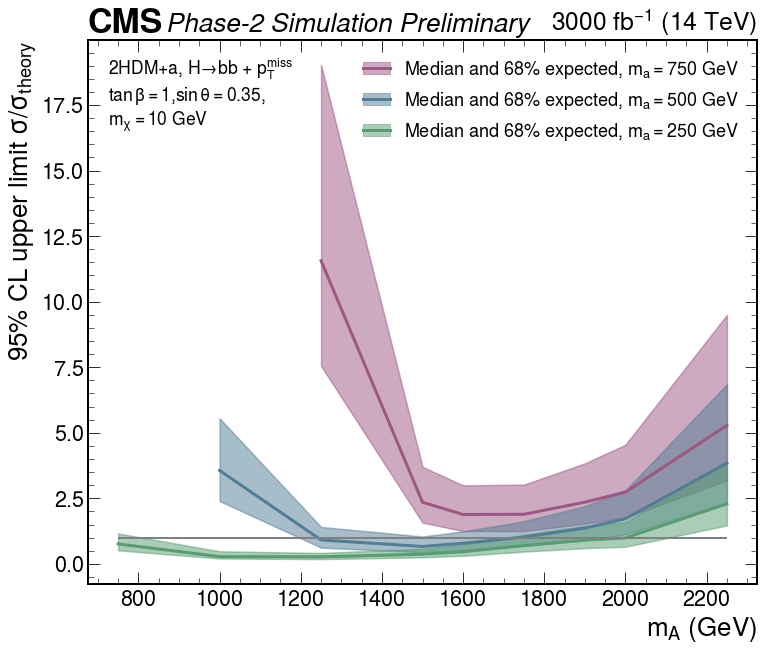
\includegraphics[width=0.5\textwidth]{Chapters/Results/lim_scan.png}
\caption{The expected limits on the 2HDM+a model of DM production in association with h $\to$ b$\bar{\mathrm{b}}$+\ptmiss. The 2HDM+a model parameters have been set at $\tan\beta = 1$, $\sin\theta = 0.35$, and $m_\chi= \GeV{10}$. The shaded regions give the 1$\sigma$ uncertainty in the limit.}
\label{fig:limits}
\end{figure}

For $m_\mathrm{a} = \GeV{250}$ and $m_\mathrm{A}$ between $1000$ and $\GeV{1600}$, the expected significance of these points could be at or above 5$\sigma$ if a significant excess is observed, as shown in \cref{fig:sig}.

\begin{figure}[ht]
\centering
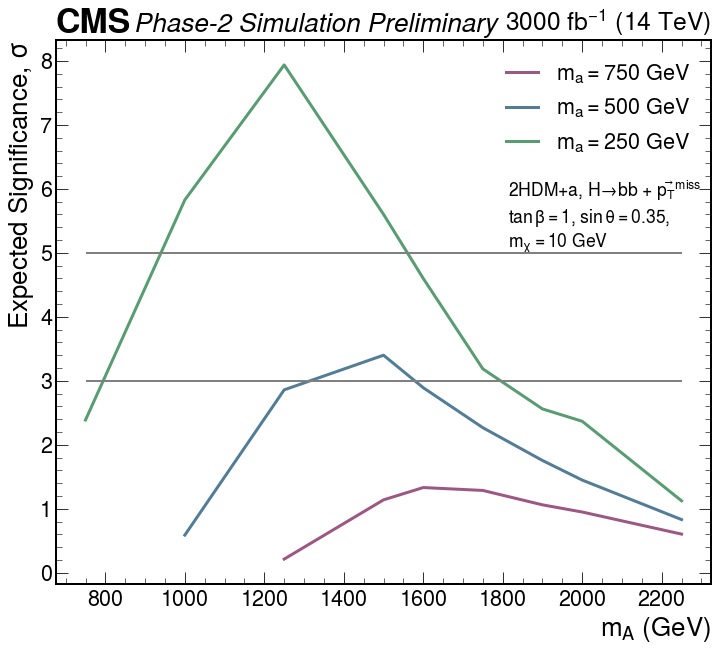
\includegraphics[width=0.5\textwidth]{Chapters/Results/sig_scan.png}
\caption{The expected significance of the 2HDM+a model of DM production in association with h $\to$ b$\bar{\mathrm{b}}$+\ptmiss. The 2HDM+a model parameters have been set at $\tan\beta = 1$, $\sin\theta = 0.35$, and $m_\chi= \GeV{10}$.}
\label{fig:sig}
\end{figure}

\section{Conclusions}
The HL-LHC will have increased sensitivity to new physics. In particular, a search probing a mono-Higgs plus \ptmiss final state where the Higgs decays to a b quark-antiquark pair will have greater sensitivity to new physics than before. Because of the increased luminosity of the collider, it is possible to probe regions that would have suffered from large statistical uncertainties, bringing further resolution to constraints on parameters of these models. The Phase-2 upgrades to CMS will allow the detector to handle the increased luminosity of the detector, ensuring the sensitivity at the HL-LHC is equal or greater than during Run 2. Additionally, upgrades to the geometry and improvements to the detector systems will allow for better exclusion of backgrounds to many searches for new physics, further increasing the sensitivity. In the case of the h $\to$ b$\bar{\mathrm{b}}$+\ptmiss final state, this analysis indicates that the expected limits would allow for further exclusion of parameter masses while establishing the first limits on higher values of the mass of the pseudoscalar A. In the case of observation of excess at the HL-LHC, there is a region of the parameter space for which this observation would be a discovery-level significance. This search could also be expanded upon. The lower mass parameter space could be explored by looking at lower-momentum Higgs bosons, increasing the sensitivity of the parameters for lower $m_\mathrm{A}$. Similarly, exploring final states with lower \ptmiss would increase the sensitivity of this search. Additionally, the parameter space could be explored further by varying the values of $\tan\beta$ or $\sin\theta$. Furthermore, this final state could be analyzed in terms of other models, such as the baryonic \Zp or \Zp-2HDM models. Regardless of the outcome, such a search would bring researchers closer to understanding the nature of dark matter. The mono-Higgs final state should be explored at the HL-LHC.

\appendix
\chapter{Monte Carlo Samples}
\label{app:samples}
The following samples were used in this analysis. Further description of the sample generation can be found in \cref{chap:datasets}.

\begin{table}
    \caption{Simulated background samples and cross sections.}
    \begin{center}
    \begin{adjustbox}{width=\textwidth}
    \begin{tabular}{|l|l|}
        \hline

        Dataset & x-sec (pb) \\ \hline

    TT\_TuneCUETP8M2T4\_14TeV-powheg-pythia8\_200PU               & 984.5 \\
TT\_Mtt1000toInf\_TuneCUETP8M1\_14TeV-powheg-pythia8\_200PU                     & 26.48 \\
ST\_tW\_antitop\_5f\_inclusiveDecays\_14TeV-powheg-pythia8\_TuneCUETP8M1\_200PU & 45.02 \\
ST\_tW\_top\_5f\_inclusiveDecays\_14TeV-powheg-pythia8\_TuneCUETP8M1\_200PU     & 45.06 \\
ST\_tch\_14TeV\_antitop\_incl-powheg-pythia8-madspin\_200PU                     & 29.2 \\
ST\_tch\_14TeV\_top\_incl-powheg-pythia8-madspin\_200PU                         & 48.03 \\
WJetsToLNu\_TuneCUETP8M1\_14TeV-madgraphMLM-pythia8\_200PU             & 71370 \\
WJetsToLNu\_GenMET-100\_TuneCUETP8M1\_14TeV-madgraphMLM-pythia8\_200PU & 236.8 \\
ZJetsToNuNu\_HT-100To200\_14TeV-madgraph\_200PU  & 305.3    \\
ZJetsToNuNu\_HT-200To400\_14TeV-madgraph\_200PU  & 86.35    \\
ZJetsToNuNu\_HT-400To600\_14TeV-madgraph\_200PU  & 12.05    \\
ZJetsToNuNu\_HT-600To800\_14TeV-madgraph\_200PU  & 3.085    \\
ZJetsToNuNu\_HT-800To1200\_14TeV-madgraph\_200PU & 1.439    \\
ZJetsToNuNu\_HT-800To1200\_14TeV-madgraph\_200PU & 0.3446   \\
ZJetsToNuNu\_HT2500toInf\_HLLHC                  & 0.008571 \\
QCD\_bEnriched\_HT200to300\_TuneCUETP8M1\_14TeV-madgraphMLM-pythia8\_200PU   & 101700 \\
QCD\_bEnriched\_HT300to500\_TuneCUETP8M1\_14TeV-madgraphMLM-pythia8\_200PU   & 21180  \\
QCD\_bEnriched\_HT500to700\_TuneCUETP8M1\_14TeV-madgraphMLM-pythia8\_200PU   & 1923   \\
QCD\_bEnriched\_HT700to1000\_TuneCUETP8M1\_14TeV-madgraphMLM-pythia8\_200PU  & 395.3  \\
QCD\_bEnriched\_HT1000to1500\_TuneCUETP8M1\_14TeV-madgraphMLM-pythia8\_200PU & 65.02  \\
QCD\_bEnriched\_HT1500to2000\_TuneCUETP8M1\_14TeV-madgraphMLM-pythia8\_200PU & 5.856  \\
QCD\_bEnriched\_HT2000toInf\_TuneCUETP8M1\_14TeV-madgraphMLM-pythia8\_200PU  & 1.115  \\
ZH\_HToBB\_ZToNuNu\_M125\_13TeV\_powheg\_pythia8\_200PU     & 0.1634 \\
WplusH\_HToBB\_WToLNu\_M125\_14TeV\_powheg\_pythia8\_200PU  & 0.2942 \\
WminusH\_HToBB\_WToLNu\_M125\_14TeV\_powheg\_pythia8\_200PU & 0.1872 \\
\hline
    \end{tabular}
    \end{adjustbox}
    \end{center}

    \label{tab:backgrounds}
\end{table}

\begin{table}
    \caption{Simulated signal samples and cross sections.}
    \begin{center}
    \begin{adjustbox}{width=\textwidth}
    \begin{tabular}{|l|l|}
        \hline

        Dataset & x-sec (pb) \\ \hline
        2HDMa\_bb\_sinp\_0.35\_tanb\_1.0\_mXd\_10\_MH3\_1000\_MH4\_150\_MH2\_1000\_MHC\_1000 & 0.0005006   \\
        2HDMa\_gg\_sinp\_0.35\_tanb\_1.0\_mXd\_10\_MH3\_1000\_MH4\_150\_MH2\_1000\_MHC\_1000 & 0.05146     \\
        2HDMa\_bb\_sinp\_0.35\_tanb\_1.0\_mXd\_10\_MH3\_1500\_MH4\_150\_MH2\_1500\_MHC\_1500 & 0.0005006   \\
        2HDMa\_gg\_sinp\_0.35\_tanb\_1.0\_mXd\_10\_MH3\_1500\_MH4\_150\_MH2\_1500\_MHC\_1500 & 0.04672     \\
        2HDMa\_bb\_sinp\_0.35\_tanb\_1.0\_mXd\_10\_MH3\_750\_MH4\_250\_MH2\_750\_MHC\_750    & 0.0002679   \\
        2HDMa\_gg\_sinp\_0.35\_tanb\_1.0\_mXd\_10\_MH3\_750\_MH4\_250\_MH2\_750\_MHC\_750    & 0.1072      \\
        2HDMa\_bb\_sinp\_0.35\_tanb\_1.0\_mXd\_10\_MH3\_1000\_MH4\_250\_MH2\_1000\_MHC\_1000 & 0.0002294   \\
        2HDMa\_gg\_sinp\_0.35\_tanb\_1.0\_mXd\_10\_MH3\_1000\_MH4\_250\_MH2\_1000\_MHC\_1000 & 0.03413     \\
        2HDMa\_bb\_sinp\_0.35\_tanb\_1.0\_mXd\_10\_MH3\_1250\_MH4\_250\_MH2\_1250\_MHC\_1250 & 0.0002007   \\
        2HDMa\_gg\_sinp\_0.35\_tanb\_1.0\_mXd\_10\_MH3\_1250\_MH4\_250\_MH2\_1250\_MHC\_1250 & 0.009852    \\
        2HDMa\_bb\_sinp\_0.35\_tanb\_1.0\_mXd\_10\_MH3\_1500\_MH4\_250\_MH2\_1500\_MHC\_1500 & 0.0001742   \\
        2HDMa\_gg\_sinp\_0.35\_tanb\_1.0\_mXd\_10\_MH3\_1500\_MH4\_250\_MH2\_1500\_MHC\_1500 & 0.0176      \\
        2HDMa\_bb\_sinp\_0.35\_tanb\_1.0\_mXd\_10\_MH3\_1600\_MH4\_250\_MH2\_1600\_MHC\_1600 & 0.0001634   \\
        2HDMa\_gg\_sinp\_0.35\_tanb\_1.0\_mXd\_10\_MH3\_1600\_MH4\_250\_MH2\_1600\_MHC\_1600 & 0.03055     \\
        2HDMa\_bb\_sinp\_0.35\_tanb\_1.0\_mXd\_10\_MH3\_1750\_MH4\_250\_MH2\_1750\_MHC\_1750 & 0.000147    \\
        2HDMa\_gg\_sinp\_0.35\_tanb\_1.0\_mXd\_10\_MH3\_1750\_MH4\_250\_MH2\_1750\_MHC\_1750 & 0.06268     \\
        2HDMa\_bb\_sinp\_0.35\_tanb\_1.0\_mXd\_10\_MH3\_1900\_MH4\_250\_MH2\_1900\_MHC\_1900 & 0.0001304   \\
        2HDMa\_gg\_sinp\_0.35\_tanb\_1.0\_mXd\_10\_MH3\_1900\_MH4\_250\_MH2\_1900\_MHC\_1900 & 0.1132      \\
        2HDMa\_bb\_sinp\_0.35\_tanb\_1.0\_mXd\_10\_MH3\_2000\_MH4\_250\_MH2\_2000\_MHC\_2000 & 0.0001193   \\
        2HDMa\_gg\_sinp\_0.35\_tanb\_1.0\_mXd\_10\_MH3\_2000\_MH4\_250\_MH2\_2000\_MHC\_2000 & 0.1587      \\
        2HDMa\_bb\_sinp\_0.35\_tanb\_1.0\_mXd\_10\_MH3\_2250\_MH4\_250\_MH2\_2250\_MHC\_2250 & 0.00009152  \\
        2HDMa\_gg\_sinp\_0.35\_tanb\_1.0\_mXd\_10\_MH3\_2250\_MH4\_250\_MH2\_2250\_MHC\_2250 & 0.3233      \\
        2HDMa\_bb\_sinp\_0.35\_tanb\_1.0\_mXd\_10\_MH3\_1000\_MH4\_500\_MH2\_1000\_MHC\_1000 & 0.00002317  \\
        2HDMa\_gg\_sinp\_0.35\_tanb\_1.0\_mXd\_10\_MH3\_1000\_MH4\_500\_MH2\_1000\_MHC\_1000 & 0.01389     \\
        2HDMa\_bb\_sinp\_0.35\_tanb\_1.0\_mXd\_10\_MH3\_1250\_MH4\_500\_MH2\_1250\_MHC\_1250 & 0.0000191   \\
        2HDMa\_gg\_sinp\_0.35\_tanb\_1.0\_mXd\_10\_MH3\_1250\_MH4\_500\_MH2\_1250\_MHC\_1250 & 0.005726    \\
        2HDMa\_bb\_sinp\_0.35\_tanb\_1.0\_mXd\_10\_MH3\_1500\_MH4\_500\_MH2\_1500\_MHC\_1500 & 0.00001582  \\
        2HDMa\_gg\_sinp\_0.35\_tanb\_1.0\_mXd\_10\_MH3\_1500\_MH4\_500\_MH2\_1500\_MHC\_1500 & 0.002497    \\
        2HDMa\_bb\_sinp\_0.35\_tanb\_1.0\_mXd\_10\_MH3\_1600\_MH4\_500\_MH2\_1600\_MHC\_1600 & 0.00001469  \\
        2HDMa\_gg\_sinp\_0.35\_tanb\_1.0\_mXd\_10\_MH3\_1600\_MH4\_500\_MH2\_1600\_MHC\_1600 & 0.002423    \\
        2HDMa\_bb\_sinp\_0.35\_tanb\_1.0\_mXd\_10\_MH3\_1750\_MH4\_500\_MH2\_1750\_MHC\_1750 & 0.0000131   \\
        2HDMa\_gg\_sinp\_0.35\_tanb\_1.0\_mXd\_10\_MH3\_1750\_MH4\_500\_MH2\_1750\_MHC\_1750 & 0.003683    \\
        2HDMa\_bb\_sinp\_0.35\_tanb\_1.0\_mXd\_10\_MH3\_1900\_MH4\_500\_MH2\_1900\_MHC\_1900 & 0.00001156  \\
        2HDMa\_gg\_sinp\_0.35\_tanb\_1.0\_mXd\_10\_MH3\_1900\_MH4\_500\_MH2\_1900\_MHC\_1900 & 0.006717    \\
        2HDMa\_bb\_sinp\_0.35\_tanb\_1.0\_mXd\_10\_MH3\_2000\_MH4\_500\_MH2\_2000\_MHC\_2000 & 0.00001057  \\
        2HDMa\_gg\_sinp\_0.35\_tanb\_1.0\_mXd\_10\_MH3\_2000\_MH4\_500\_MH2\_2000\_MHC\_2000 & 0.009834    \\
        2HDMa\_bb\_sinp\_0.35\_tanb\_1.0\_mXd\_10\_MH3\_2250\_MH4\_500\_MH2\_2250\_MHC\_2250 & 0.000008163 \\
        2HDMa\_gg\_sinp\_0.35\_tanb\_1.0\_mXd\_10\_MH3\_2250\_MH4\_500\_MH2\_2250\_MHC\_2250 & 0.02217     \\
        2HDMa\_bb\_sinp\_0.35\_tanb\_1.0\_mXd\_10\_MH3\_1250\_MH4\_750\_MH2\_1250\_MHC\_1250 & 0.000003398 \\
        2HDMa\_gg\_sinp\_0.35\_tanb\_1.0\_mXd\_10\_MH3\_1250\_MH4\_750\_MH2\_1250\_MHC\_1250 & 0.002491    \\
        2HDMa\_bb\_sinp\_0.35\_tanb\_1.0\_mXd\_10\_MH3\_1500\_MH4\_750\_MH2\_1500\_MHC\_1500 & 0.000002785 \\
        2HDMa\_gg\_sinp\_0.35\_tanb\_1.0\_mXd\_10\_MH3\_1500\_MH4\_750\_MH2\_1500\_MHC\_1500 & 0.001332    \\
        2HDMa\_bb\_sinp\_0.35\_tanb\_1.0\_mXd\_10\_MH3\_1600\_MH4\_750\_MH2\_1600\_MHC\_1600 & 0.000002528 \\
        2HDMa\_gg\_sinp\_0.35\_tanb\_1.0\_mXd\_10\_MH3\_1600\_MH4\_750\_MH2\_1600\_MHC\_1600 & 0.001016    \\
        2HDMa\_bb\_sinp\_0.35\_tanb\_1.0\_mXd\_10\_MH3\_1750\_MH4\_750\_MH2\_1750\_MHC\_1750 & 0.000002193 \\
        2HDMa\_gg\_sinp\_0.35\_tanb\_1.0\_mXd\_10\_MH3\_1750\_MH4\_750\_MH2\_1750\_MHC\_1750 & 0.0007266   \\
        2HDMa\_bb\_sinp\_0.35\_tanb\_1.0\_mXd\_10\_MH3\_1900\_MH4\_750\_MH2\_1900\_MHC\_1900 & 0.000001897 \\
        2HDMa\_gg\_sinp\_0.35\_tanb\_1.0\_mXd\_10\_MH3\_1900\_MH4\_750\_MH2\_1900\_MHC\_1900 & 0.0006894   \\
        2HDMa\_bb\_sinp\_0.35\_tanb\_1.0\_mXd\_10\_MH3\_2000\_MH4\_750\_MH2\_2000\_MHC\_2000 & 0.000001719 \\
        2HDMa\_gg\_sinp\_0.35\_tanb\_1.0\_mXd\_10\_MH3\_2000\_MH4\_750\_MH2\_2000\_MHC\_2000 & 0.000809    \\
        2HDMa\_bb\_sinp\_0.35\_tanb\_1.0\_mXd\_10\_MH3\_2250\_MH4\_750\_MH2\_2250\_MHC\_2250 & 0.000001327 \\
        2HDMa\_gg\_sinp\_0.35\_tanb\_1.0\_mXd\_10\_MH3\_2250\_MH4\_750\_MH2\_2250\_MHC\_2250 & 0.001565    \\

  
\hline
   
    \end{tabular}
    \end{adjustbox}
    \end{center}
    \label{tab:signals}
\end{table}



\titleformat{\chapter}{}{}{0em}{\bf\LARGE}

\clearpage
\addcontentsline{toc}{chapter}{Acknowledgements}
\chapter*{Acknowledgements}
I would like to thank Professor Indara Suarez and Doctor Daniel Spitzbart for their invaluable help in the research for and writing of this thesis. Without their direction and input, I would not have been able to complete the analysis that forms the backbone of this thesis. I would additionally like to thank the CMS Collaboration. Finally, I would like to thank my friends and family for their support and for helping to keep me sane during my research and studies.

\bibliographystyle{cms_unsrt}
\clearpage
\addcontentsline{toc}{chapter}{Bibliography}
\bibliography{hbbmet}

\end{document}